\documentclass{svmult}

\usepackage{mathptmx}       % selects Times Roman as basic font
\usepackage{helvet}         % selects Helvetica as sans-serif font
\usepackage{courier}        % selects Courier as typewriter font
\usepackage{type1cm}        % activate if the above 3 fonts are
                            % not available on your system
\usepackage[numbers]{natbib}
%
\usepackage{makeidx}         % allows index generation
\usepackage{graphicx}        % standard LaTeX graphics tool
                             % when including figure files
\usepackage{multicol}        % used for the two-column index
\usepackage[bottom]{footmisc}% places footnotes at page bottom
\usepackage{listings}
\usepackage{color}
\usepackage{tikz}
\usepackage{amsmath}
\usepackage{amssymb}

\usepackage{footmisc}
\usepackage{import}
\usepackage{enumitem}
\usepackage{booktabs}
\usepackage{lipsum}

\usepackage{capt-of}
\usepackage{float}
\usepackage{tabularx}
\usepackage{watermark} % titlepage image
\usepackage{booktabs}
\usepackage[hidelinks]{hyperref}
\usepackage[parfill]{parskip}
%\usepackage[nottoc]{tocbibind}
\usepackage{tocloft}
\usepackage[disable]{todonotes}

\usepackage{microtype} % Improves spacing
\usepackage{fancyhdr} 
\fancyhead[L]{\rightmark}
\fancyhead[R]{\leftmark} 
\usepackage[toc,page]{appendix}

\usetikzlibrary{shapes.misc, shapes.geometric, arrows, positioning, calc, decorations.markings}
\tikzset{
  query/.style={draw=blue!10,thick,fill=blue!2,inner sep=.15cm},
  answer/.style={rectangle,draw=black!10,fill=gray!4},
  icon/.style={circle,thick,fill=blue!20,draw=blue!30,inner sep=.05cm,font=\bfseries},
  data/.style={draw=easeblue!30,thick,fill=easeblue!10,inner sep=.15cm},
  owlclass/.style={draw=easeblue!40,fill=easeblue!10,text=easeblue,font=\bf,minimum width=2.5cm},
  owlclass_f/.style={owlclass,text width=2.0cm,minimum width=2.0cm,text badly centered},
  relation/.style={thick,-latex,black,font=\it\scriptsize},
  relationxl/.style={relation,bend right=20},
  relationxr/.style={relation,bend left=-20},
}
\pgfdeclarelayer{back}
\pgfdeclarelayer{front}
\pgfsetlayers{back,main,front}

\lstdefinelanguage[OWL]{XML} {morekeywords={Individual,ObjectProperty,Types,Facts,Class,SubClassOf,Domain,Range,SubPropertyOf,EquivalentTo}}
\lstdefinestyle{OWL}    {language=[OWL]XML,    lineskip=0.2ex, fontadjust=true, basicstyle={\scriptsize \nopagebreak[4]}}
\lstdefinestyle{Prolog} {language=Prolog, lineskip=0.2ex, fontadjust=true, basicstyle={\scriptsize \nopagebreak[4]}, commentstyle=\scriptsize,
    morekeywords={entity, occurs, holds, show, append, forall, findall, member}}

\graphicspath{img}

\lstdefinestyle{lispcode}{
	backgroundcolor=\color{lightgray},   
	commentstyle=\color{codegreen},
	keywordstyle=\color{magenta},
	numberstyle=\tiny\color{white},
	stringstyle=\color{purple},
	basicstyle=\ttfamily\footnotesize,
	breakatwhitespace=false,         
	breaklines=true,                 
	captionpos=b,                    
	keepspaces=true,                 
	numbers=left,                    
	numbersep=5pt,                  
	showspaces=false,                
	showstringspaces=false,
	showtabs=false,                  
	tabsize=2
}

\definecolor{ease_lightblue}{HTML}{D4E5EF}
\definecolor{ease_darkblue}{HTML}{144F78}
\colorlet{easeblue}{ease_darkblue}
\colorlet{robotblue}{ease_darkblue}

% json data display 
\colorlet{json_punctuation}{red!60!black}
\definecolor{json_background}{HTML}{EEEEEE}
\definecolor{json_delim}{RGB}{20,105,176}
\colorlet{json_numb}{magenta!60!black}

\lstdefinelanguage{json}{
	basicstyle=\normalfont\ttfamily,
	numbers=left,
	numberstyle=\scriptsize,
	stepnumber=1,
	numbersep=8pt,
	showstringspaces=false,
	breaklines=true,
	frame=lines,
	backgroundcolor=\color{json_background},
	literate=
	*{0}{{{\color{json_numb}0}}}{1}
	{1}{{{\color{json_numb}1}}}{1}
	{2}{{{\color{json_numb}2}}}{1}
	{3}{{{\color{json_numb}3}}}{1}
	{4}{{{\color{json_numb}4}}}{1}
	{5}{{{\color{json_numb}5}}}{1}
	{6}{{{\color{json_numb}6}}}{1}
	{7}{{{\color{json_numb}7}}}{1}
	{8}{{{\color{json_numb}8}}}{1}
	{9}{{{\color{json_numb}9}}}{1}
	{:}{{{\color{json_punctuation}{:}}}}{1}
	{,}{{{\color{json_punctuation}{,}}}}{1}
	{\{}{{{\color{json_delim}{\{}}}}{1}
	{\}}{{{\color{json_delim}{\}}}}}{1}
	{[}{{{\color{json_delim}{[}}}}{1}
	{]}{{{\color{json_delim}{]}}}}{1},
}

%\newcommand{\todo}[1]{\textcolor{red}{\textbf{TODO}: #1}}
%\lstdefinelanguage[OWL]{XML} {morekeywords={Individual,ObjectProperty,Types,Facts,Class,SubClassOf,Domain,Range,SubPropertyOf,EquivalentTo}}
%\lstdefinestyle{OWL}    {language=[OWL]XML,    lineskip=0.2ex, fontadjust=true, basicstyle={\scriptsize \nopagebreak[4]}}
%\lstdefinestyle{Prolog} {language=Prolog, lineskip=0.2ex, fontadjust=true, basicstyle={\scriptsize \nopagebreak[4]}, commentstyle=\scriptsize,
%    morekeywords={entity, occurs, holds, show, append, forall, findall, member}}

\title*{NEEM Handbook}
\author{The EASE Researchers}
\institute{CRC Everyday Activity Science and Engineering (EASE)\\ University Bremen, Am Fallturm 1, 28359 Bremen\\ \texttt{ai-office@cs.uni-bremen.de}}
\thiswatermark{
 \centering
 \put(0,-630){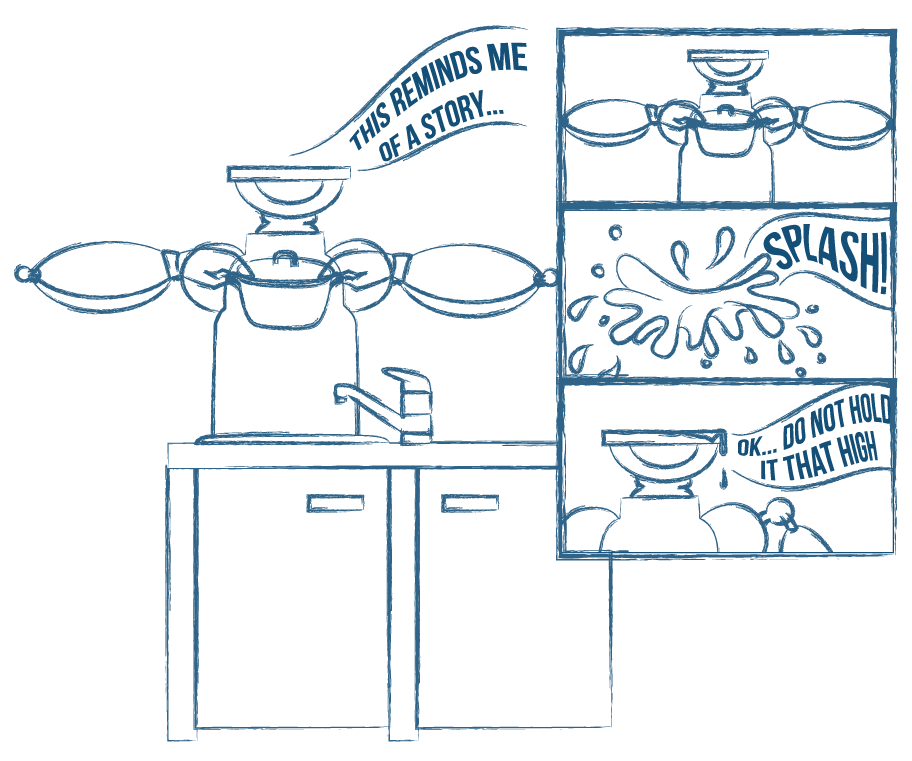
\includegraphics[width=12cm]{img/NarrativesStory.png}}
 \put(340,-10){
\includegraphics[width=4.0cm]{img/ease-logo.pdf}}}

\renewcommand\thesection{\thechapter.\arabic{section}}

% TODO: use current SOMA version?
\newcommand{\neemversion}{1.0~}
\newcommand{\neemexp}{NEEM-experience~}
\newcommand{\neemexps}{NEEM-experiences~}
\newcommand{\neemnar}{NEEM-narrative~}
\newcommand{\neembak}{NEEM-background~}
\newcommand{\neem}{NEEM~}
\newcommand{\neems}{NEEMs~}
\newcommand{\neemhub}{NEEM-hub~}
\newcommand{\tf}{tf~}
\newcommand{\openease}{openEASE~}
\newcommand{\ease}{EASE~}
\newcommand{\mongodb}{MongoDB~}
\newcommand{\cram}{CRAM~}
\newcommand{\knowrob}{KnowRob~}
\newcommand{\owl}{OWL~}
\newcommand{\pr}{PR2~}
\newcommand{\qudt}{Qudt~}
\newcommand{\boxy}{Boxy~}
\newcommand{\eg}{e.g.~}
\newcommand{\ros}{ROS~}
\newcommand{\soma}{SOMA~}
\newcommand{\dul}{DUL~}
\newcommand{\easeOwl}{EASE.owl~}
\newcommand{\easeAct}{EASE-ACT.owl~}
\newcommand{\easeObj}{EASE-OBJ.owl~}
\newcommand{\cramOwl}{cram\_failures.owl}
\newcommand{\cramentitytoreplace}[1]{\textless #1\textgreater}
\newcommand{\cramloggerpackage}{"cram-cloud-logger"~}
\newcommand{\owlClass}[1]{\textit{#1}}
\newcommand{\owlPredicate}[1]{\textit{#1}}
\newcommand{\f}{\mkern-2mu f\mkern-3mu}
\newcommand{\abox}{\mathcal{A}}
\newcommand{\tbox}{\mathcal{T}}
\newcommand{\concept}[1]{\emph{#1}}
\newcommand{\relation}[1]{\emph{#1}}

\makeatletter
\newcommand{\chapterauthor}[1]{%
  {\parindent0pt\vspace*{-25pt}%
  \linespread{1.1}\large\scshape#1%
  \par\nobreak\vspace*{35pt}}
  \@afterheading%
}
\makeatother

\renewcommand\tabularxcolumn[1]{m{#1}}
\newcolumntype{Y}{>{\centering\arraybackslash}X}
% % % % % % % % % % % % % % % % % % % % % % % %
% % % Prelude
% % % % % % % % % % % % % % % % % % % % % % % %
\newcommand{\givenODPNAME}{}
\newcommand{\givenODPINTENT}{}
\newcommand{\givenODPDEFINEDIN}{}
\newcommand{\givenODPGRAPHIC}{}
\newcommand{\givenODPEXAMPLES}{}
\newcommand{\givenODPQUESTION}{}
\newcommand{\ODPINTENT}[1]     {\renewcommand{\givenODPINTENT}{#1}}
\newcommand{\ODPDEFINEDIN}[1]  {\renewcommand{\givenODPDEFINEDIN}{#1}}
\newcommand{\ODPGRAPHIC}[1]    {\renewcommand{\givenODPGRAPHIC}{#1}}
\newcommand{\ODPEXAMPLES}[1]   {\renewcommand{\givenODPEXAMPLES}{#1}}
\newcommand{\ODPQUESTION}[1]   {\renewcommand{\givenODPQUESTION}{#1}}
\newcommand{\OPDinit}{
  \renewcommand{\givenODPINTENT}{REQUIRED!}
  \renewcommand{\givenODPDEFINEDIN}{REQUIRED!}
  \renewcommand{\givenODPGRAPHIC}{REQUIRED!}
  \renewcommand{\givenODPQUESTION}{}
  \renewcommand{\givenODPEXAMPLES}{}
  \renewcommand{\labelitemi}{$\mathbf{\sqsubseteq}$}
}

\newenvironment{ODP}[1]{
\OPDinit
\renewcommand{\givenODPNAME}{#1}
}{
%\givenODPDESCRIPTION
%\begin{figure}[htb!]
\vspace{0.2cm}
\begin{minipage}{0.55\textwidth}
\fcolorbox{easeblue!40}{easeblue!10}{\begin{tabular}{ p{1.8cm} p{4.2cm} }
%\toprule
% {\it\bf Name}                 & \emph{\givenODPNAME} \\
{\noindent\color{easeblue}\it\bf Intent}               & \givenODPINTENT \\
{\noindent\color{easeblue}\it\bf Competency Questions} & \emph{\givenODPQUESTION} \\
{\noindent\color{easeblue}\it\bf Defined in}           & \givenODPDEFINEDIN \\
%\bottomrule
\end{tabular}}
\end{minipage}
\begin{minipage}{0.45\textwidth}
\begin{center}
\givenODPGRAPHIC
\end{center}
\end{minipage}
\\[0.4cm]
\fcolorbox{easeblue!40}{easeblue!10}{
	\begin{minipage}{0.96\textwidth}
		\begin{tabular}{p{4.4cm}p{6.7cm}}
		{\noindent\color{easeblue}\it\bf Expression}  &
		{\noindent\color{easeblue}\it\bf Meaning} \\
		\givenODPEXAMPLES
		\end{tabular}
	\end{minipage}
}
%\caption{\emph{The Representation of \givenODPNAME}.}
%\end{figure}
\vspace{0.2cm}
}

\setcounter{tocdepth}{3}

\begin{document}
\let\oldaddcontentsline\addcontentsline
\def\addcontentsline#1#2#3{}
\maketitle
\def\addcontentsline#1#2#3{\oldaddcontentsline{#1}{#2}{#3}}

\begin{abstract}
The Collaborative Research Center \ease is an interdisciplinary research initiative at the University of Bremen that attempts to advance our understanding of how human-scale manipulation tasks can be mastered by robotic agents.
The challenge is that the same task needs to be executed by the robot in different ways depending on, for example, what tools are available, and how the environment is shaped.
The key to solve this issue is \emph{generalization}.
However, the robot needs to know more then what step it needs to execute next -- it further needs to decide on how the next step is carried out through motions of its body, and interactions with its environment.
In this document, we will describe how these types of information are represented in the \ease system, how such data-sets are acquired, and how they are stored, maintained, and curated using a centralized web-service.
The goal of this effort is to establish representations and infrastructure for a shared experience storage with annotated data-sets of agents performing everyday activities,
and to use these data-sets as ground truth data to find generalizations that do not abstract away from movements, and naive physics.
\end{abstract}

\cleardoublepage
\tableofcontents

\pagenumbering{arabic}
\setcounter{page}{0}
\cleardoublepage
\chapter{Introduction}
\chapterauthor{D. Be{\ss}ler, S. Koralewski, M. Pomarlan}

This document, referred to as the ``\neem Handbook'' hereafter,
describes the \ease system for episodic memories of everyday activities.
%The \neem Handbook will be updated along the progress in the CRC \ease.
It is thought to provide \ease researchers with compact but still comprehensive
information about what information is contained in \neems,
how it is represented, acquired, curated and published.

\begin{figure}[h!]
\centering
\begin{tikzpicture}[
    border/.style={draw=easeblue},
    dark/.style={border,fill=easeblue!20},
    light/.style={border,fill=easeblue!10},
    lighter/.style={border,fill=easeblue!5},
    heading/.style={text=easeblue,font=\bf,text badly centered},
    label1/.style={text=easeblue,text badly centered},
    label2/.style={text=black,text badly centered,font=\it},
    label/.style={text=black,text width=1.7cm,text badly centered},
    hexagon/.style={regular polygon,regular polygon sides=6,rounded corners},
    triangle/.style={regular polygon,regular polygon sides=3,rounded corners},
    trapez/.style={font=\bf,text badly centered,trapezium,trapezium angle=60,rounded corners},
    user/.style={hexagon,lighter,minimum width=2.5cm,inner sep=0},
    img/.style={}
]
  %\draw[help lines](-4,-4)grid(4,3);
  %% outer hexagon
  \node[hexagon,dark,minimum width=5.0cm] (OUTER) {};
  \node[heading] at (0,-1.8) (ACQ) {acquisition};
  \node[heading,rotate around={120:(OUTER)},rotate=180] at (ACQ) {curation};
  \node[heading,rotate around={-120:(OUTER)},rotate=180] at (ACQ) {publication};
  %% inner triangle
  \node[triangle,light,minimum width=6.0cm] at (OUTER) (INNER) {};
  %% inner trapez
  \node[trapez,lighter,
    minimum height=21mm,yshift=-0.275cm] at (INNER.center) (LIB) {};
  \node[label,yshift=0.2cm] at (INNER) (BG) {NEEM Background};
  \node[label,below=0.2cm of BG.south,anchor=north east] (NAR) {NEEM Narrative};
  \node[label,below=0.2cm of BG.south,anchor=north west] (EXP) {NEEM Experience};
  \draw[draw=easeblue] (BG.south west) -- (BG.south east);
  \draw[draw=easeblue] (NAR.north east) -- (NAR.south east);
  %% heading
  \node[label1,text width=14mm,above=0.4cm of BG] (HUB1) {NEEM HUB};
  %%
  \node[user,text=black,anchor=north,yshift=-0.2cm,
    path picture={\node[yshift=1.8cm] at (path picture bounding box.center){
        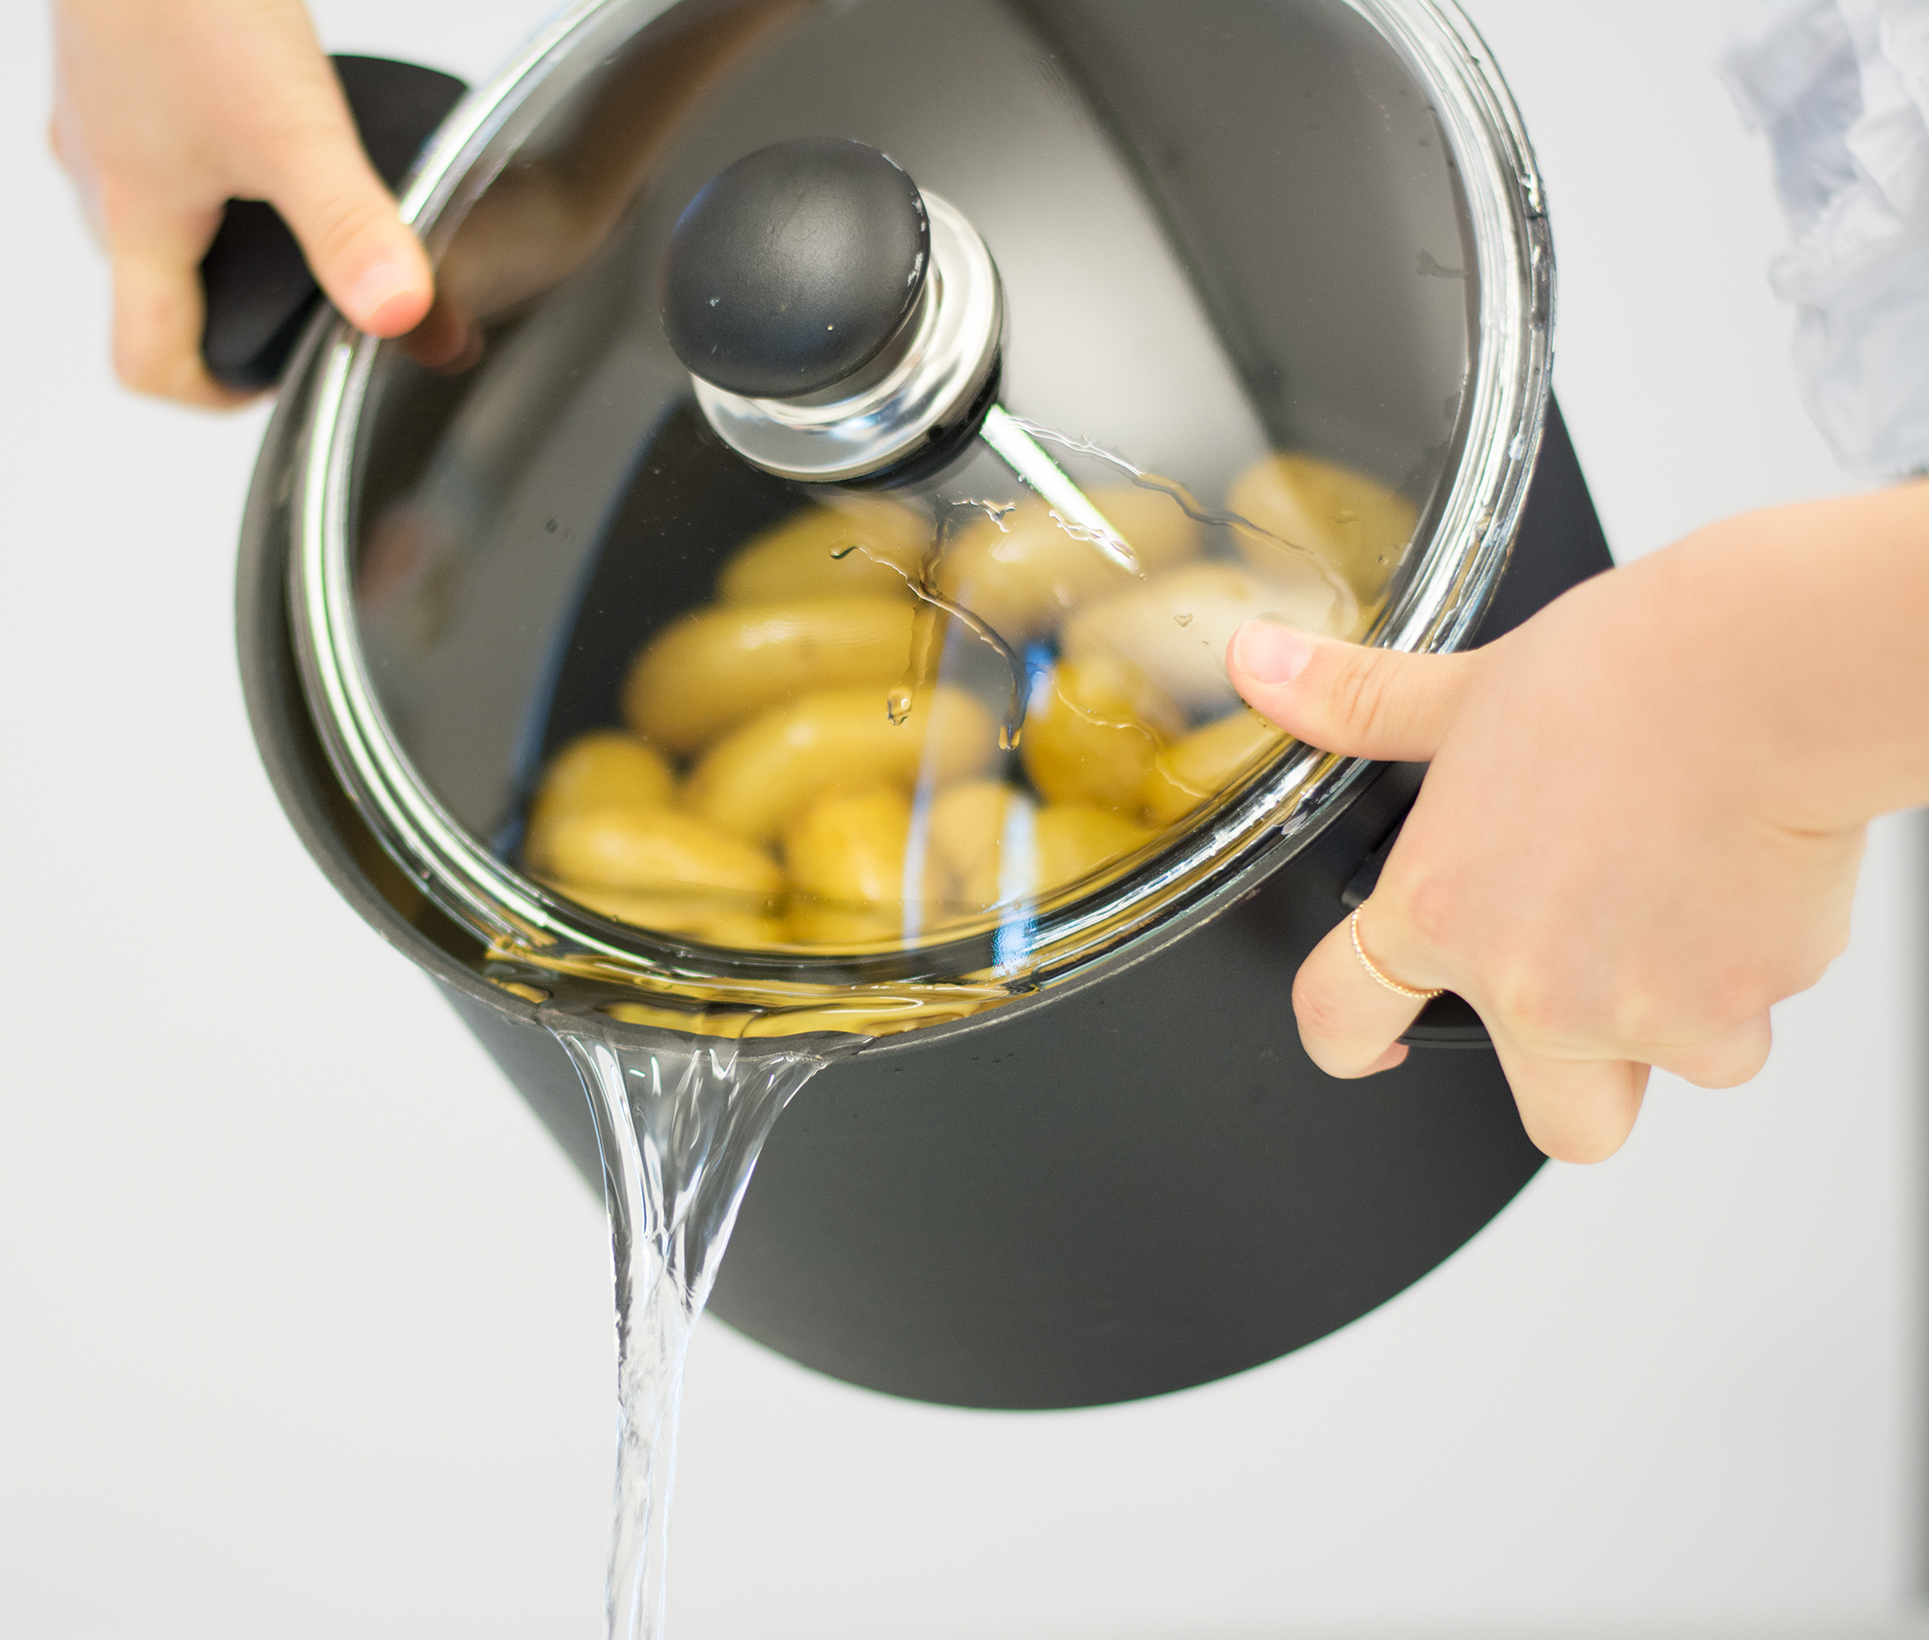
\includegraphics[width=2.55cm]{img/topf-2.jpg}
    };}
  ] at (OUTER.south) (X1) {};
  \node[user,anchor=center,yshift=-0.4cm,xshift=2.4cm,
    path picture={\node[yshift=0.0cm] at (path picture bounding box.center){
        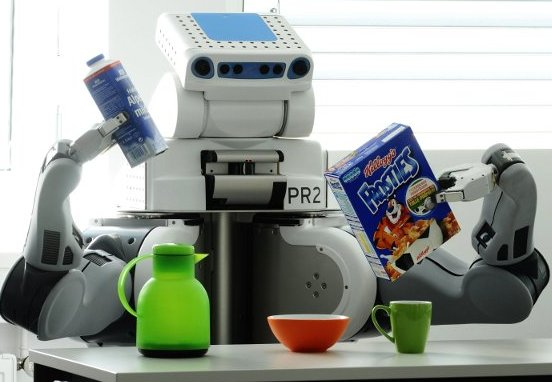
\includegraphics[height=2.55cm]{img/pr2_milk_frosties_small_top.jpg}
    };}
  ] at (X1.north) (X2) {};
  \node[user,anchor=center,yshift=-0.4cm,xshift=-2.4cm,
    path picture={\node[yshift=0.0cm] at (path picture bounding box.center){
        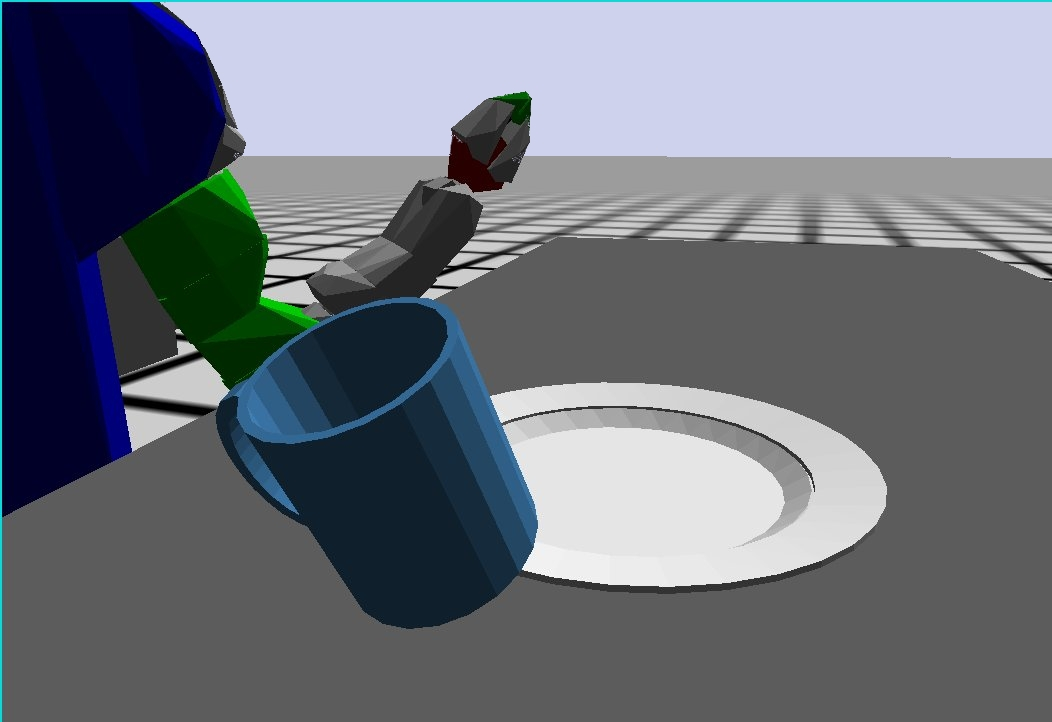
\includegraphics[height=2.55cm]{img/cup-on-plate-unstable-final.jpg}
    };}
  ] at (X1.north) (X5) {};
  \node[user,rotate around={120:(OUTER)},
    path picture={\node[yshift=0.0cm] at (path picture bounding box.center){
        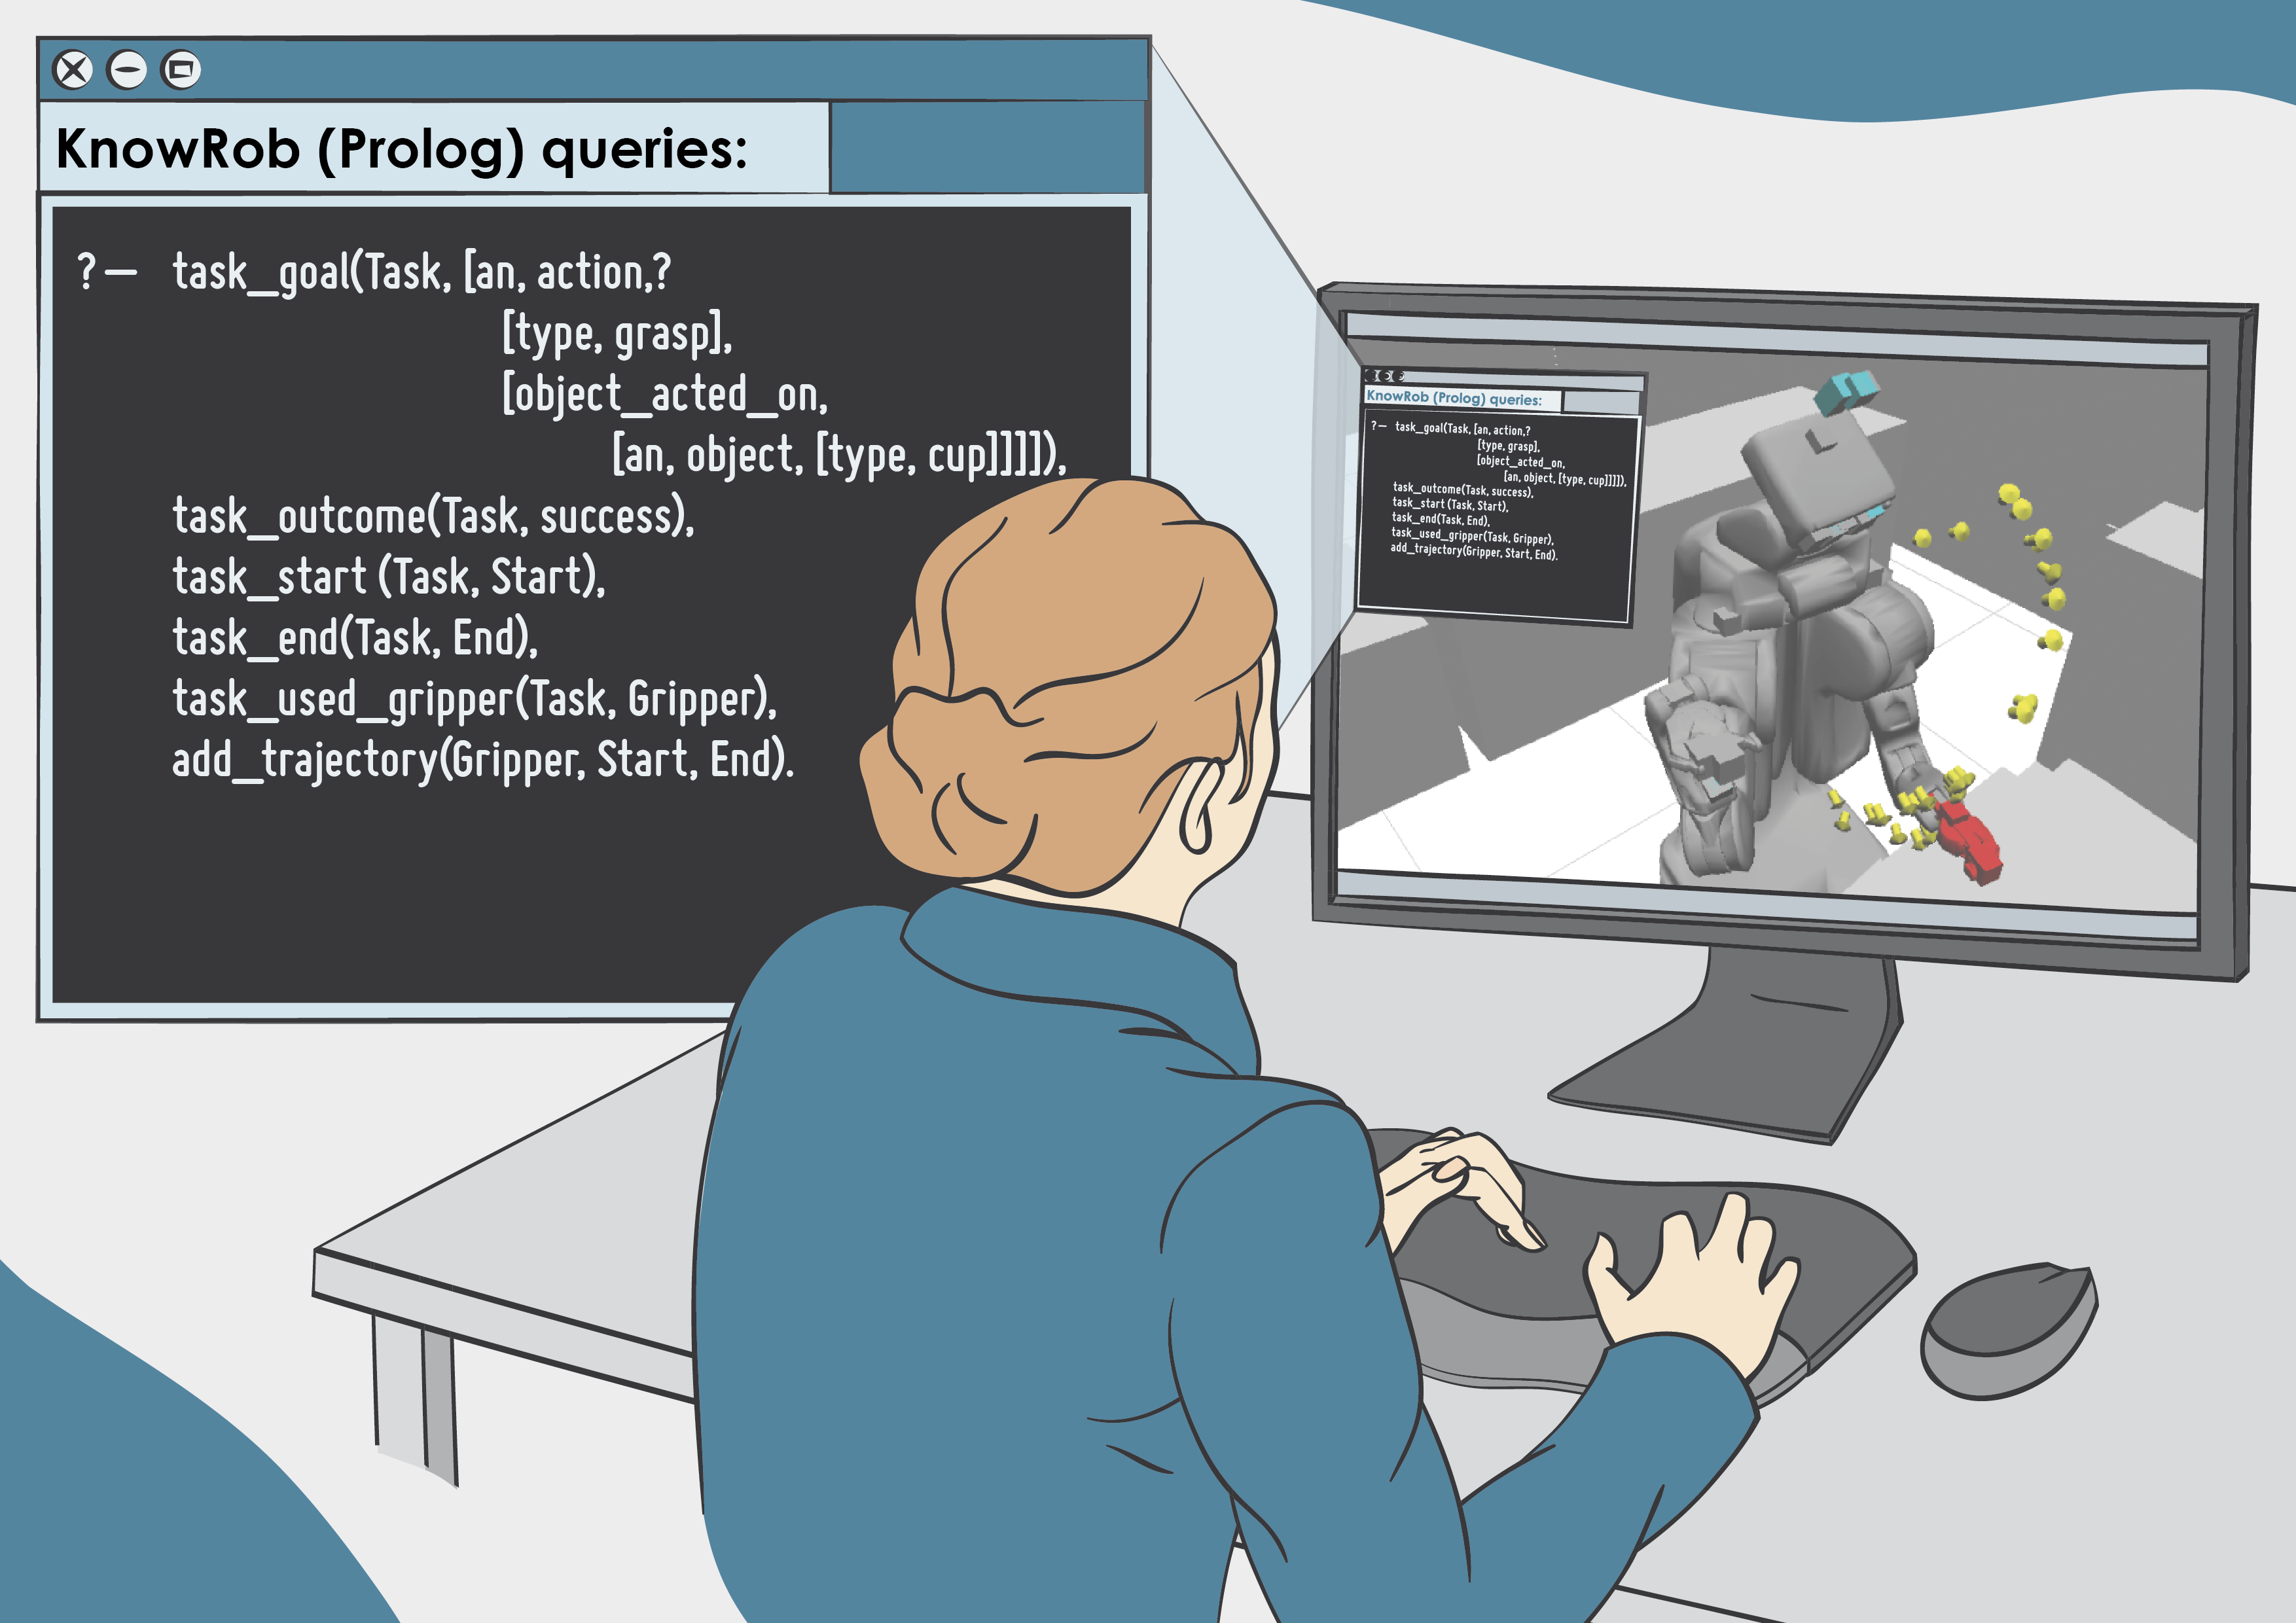
\includegraphics[height=2.55cm]{img/Programmer.png}
    };}
  ] at (X1) (X3) {};
  \node[user,rotate around={-120:(OUTER)},
    path picture={\node[yshift=0.0cm] at (path picture bounding box.center){
        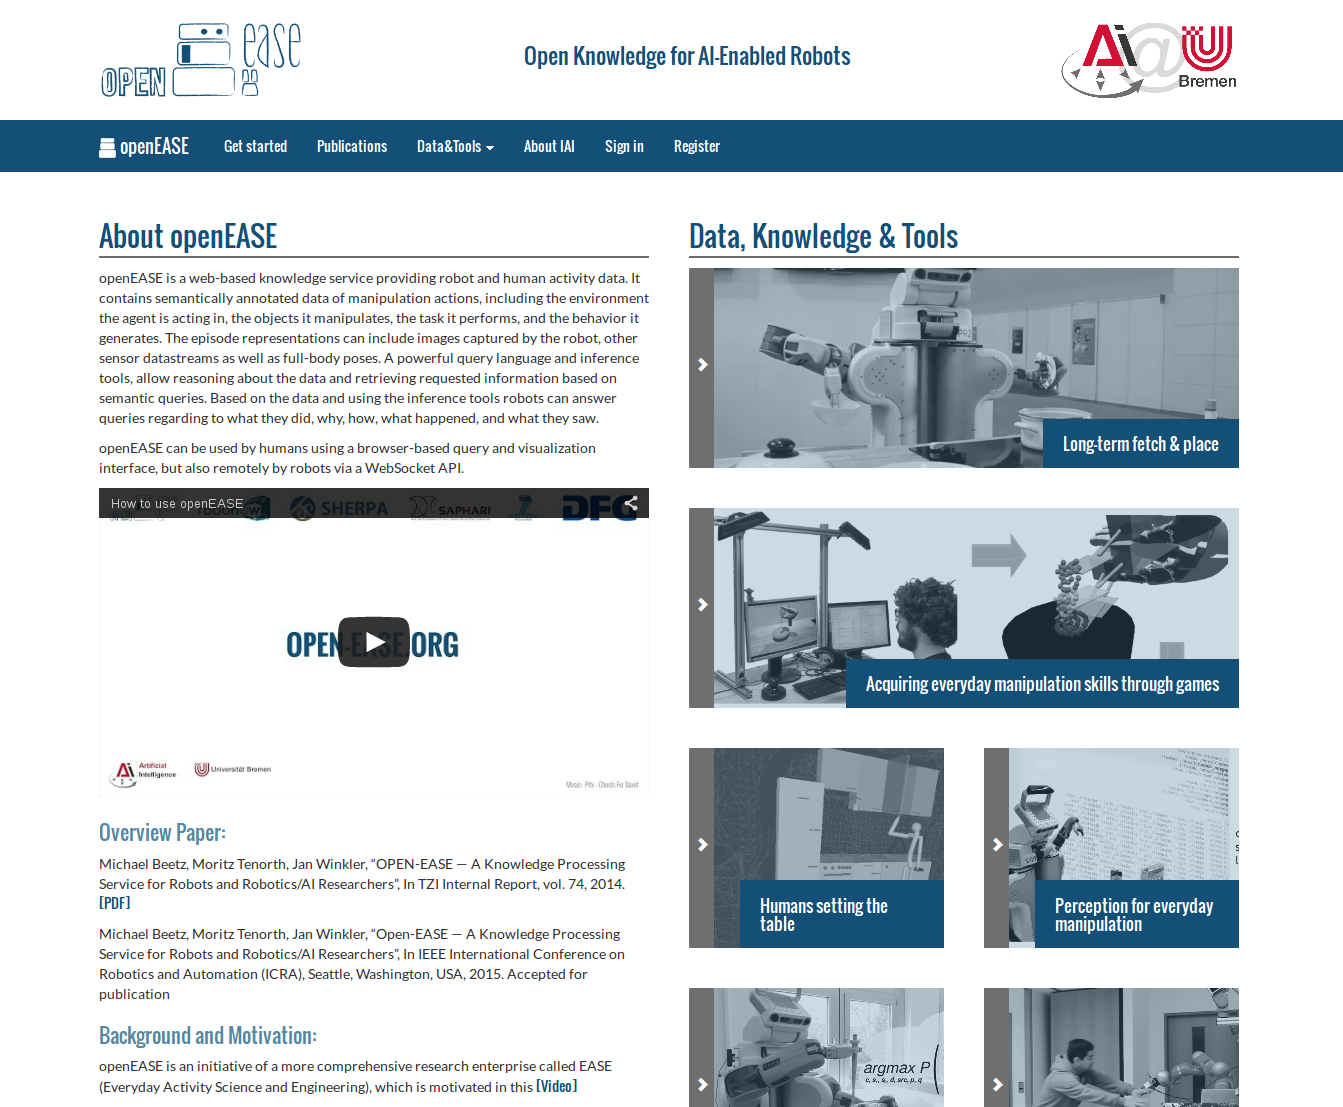
\includegraphics[height=2.55cm]{img/open-ease-web-page-full_cropped.png}
    };}
  ] at (X1) (X4) {};
  %%
  \node[label2,anchor=north] at (X1.south) {observation};
  \node[label2,anchor=north] at (X2.south) {experimentation};
  \node[label2,anchor=north] at (X5.south) {simulation};
  
\end{tikzpicture}
\caption{The EASE system for acquisition, curation and publication of episodic memories}
\label{fig:architecture}
\end{figure}

\paragraph{Narrative Enabled Episodic Memories}
% From KnowRob 2.0
When somebody talks about the deciding goal in the last soccer world championship many of us can ``replay'' the episode in our ``mind's eye''.
Those episodic memories can be seen as abstract descriptions that allow us to recall detailed pieces of information from any experienced activity.
Having those detailed memories, we can use them to learn general knowledge or map similar memories to unknown situations, so we know how to behave in the given situation.
\todo{DB: refer to Figure~\ref{fig:architecture}}

% From KnowRob 2.0
\ease integrates episodic memories deeply into the knowledge acquisition, representation, and processing system. 
For every activity the agent performs, observes, prospects and reads about, it creates an episode and stores it in its memory.
An episode is best understood as a video recording that the agent makes of the ongoing activity.
In addition, those videos are enriched with a very detailed story about the actions, motions, their purposes, effects and the agent's sensor information during the activity.

% From KnowRob 2.0
We define the episodic memories created by our system narrative-enabled episodic memories (\neems).
A \neem consists of the \emph{\neem experience} and the \emph{\neem narrative}.
The \neem experience captures low-level data such as the agent's sensor information, e.g. images and forces, and records of poses of the agent and its detected objects.
\neem experiences are linked to \neem narratives, which are stories of the episode described symbolically.
These narratives contain information regarding the tasks, the context, intended goals, observed effects, etc.
The \neemexp and \neemnar combined are so rich of information that the agent can replay an episode to experience the seen activity anytime again.

\neems are representations of experiences acquired through experimentation, reading, observing, mental simulation, etc.
The main goal is to establish a common vocabulary used to annotate experience data across different tasks, scientific disciplines, and modalities of acquisition, and to define models for the representation of experience data.
The vocabulary is not just a set of atomic labels, but each label has a formal definition in an ontology.
These definitions are done such that a set of \emph{competency questions} about an activitiy can be answered by a knowledge base that is equipped with the ontology and a collection of \neems.

The \neem model is formally defined in form of an \owl ontology which is based on the DOLCE+DnS Ultralite (DUL) upper-level ontology~\cite{DOLCE2003}.
DUL is a carefully designed ontology that seeks to model general categories underlying human cognition without making any discipline-specific assumptions.
Our extensions of DUL mainly focus on characterizing different aspects of activities that were not considered in much detail in DUL, but are relevant for the autonomous robotics scope.
These extensions are part of an ontology that we have called
\soma~\footnote{\url{https://ease-crc.github.io/soma}}.
A \neem is made of several patterns defined either in \dul or in \soma.

While it is possible to create the representations listed in this document through a custom exporter, it is not advised to do so.
Instead, it is advised to interface with the
\knowrob knowledge base~\footnote{\url{https://github.com/knowrob/knowrob}}.
\knowrob provides an interface based on predicate logics that allows to interact with \neems.
The language is a collection of predicates that can be called by users to ask certain types of competency questions covering different aspects of activitiy, or to add labels and relationships in the \neemnar.
We will provide example expressions in this document that highlight how the knowledge base can be used to interact with \neems.

% paragraph about generalizability of robot behaviour (add reference to Pratt paper ``Is a Cambrian Explosion Coming for Robotics?'')
\lipsum[4]
\todo{DB: write paragraph about generalizability, Pratt paper ``Is a Cambrian Explosion Coming for Robotics?''}

% % % % % % % % % % % % % % % % %
% % % % % % % % % % % % % % % % %
\section{Notation} % Domain of Discourse
\label{sec:notation}

In this Section, we will shortly introduce the notions and notations that are important to follow this document.
%Because in subsequent sections we will give more formal definitions for various concepts, we now review some basic notions about the main formalism we use in the ontology, as well as introduce the notation we will employ.

%%% ABOX -- TBOX
\neems are formally represented using an \emph{ontology}.
An ontology is a collection of logical axioms in some formal language such as description logic (DL).
%In the case of many ontologies available in the semantic web, as well as in the case of SOMA, this formal language is description logic, also known as DL.
The entities that can be described in DL can be either \emph{concepts} (sometimes known as \emph{classes}),
and \todo{Seba: Can we here remove individuals? It seems not very well definied that concepts are known as individuals and in the next sentence the instances are called individuals. MP: I checked the Description Logic Primer, and they use individuals. I think we should keep this.}
\emph{instances}.
An individual may belong to one or more concepts.
A concept may be subsumed by another concept.
Between individuals there may be relations called \emph{object properties},
and, in addition, an individual can also have \emph{data properties} that link it to some data values.
%As a syntactic convenience, an individual can also have ``data properties'' that link it to some alphanumeric data item which is itself not considered an individual in the ontology.
As an example, let us assume that Alice and Bob are both individuals belonging to the concept \concept{Human},
and that the object property \relation{hasChild} connects Alice to Bob,
i.e. the relation asserts that Bob is a child of Alice.
We may also know the height of Alice, which would be represented by a data property \relation{hasHeight} whose value could be a string such as \emph{1,7m} to represent that she is 1.7m tall.
%%
In the following, to make clear when we are talking about concepts and when about individuals, we will denote the set of all concepts as $\mathcal{T}$ (called the TBox), and the set of all individuals as $\mathcal{A}$ (called the ABox).
%Accordingly, there are axioms that describe concepts or object/data properties,
%and axioms that describe individuals and the relations between them.
%The set of concepts, object and data properties, and the axioms that
%define them is called the Tbox, or terminological part,
%and we will denote it by $\mathcal{T}$.
%The set of individuals and the axioms describing them is called the Abox,
%or assertion part, and we will denote it by $\mathcal{A}$.

%%% formatting
It is useful when describing concepts to emphasize the concept names such that it is clear we reference the concept, and not the colloquial word. As such, \concept{Concepts} and \relation{relations} will be written in a different font.
Note that the name of a concept always starts with an uppercase letter, whereas the name of a relation with a lowercase one.
Any word appearing in a concept or relation name after the first one will always begin with an uppercase letter.

%%% namespaces
Ontologies are meant to build on one another, and it is not uncommon for an ontology to collect thousands of concepts from external ontologies it imports.
To prevent name clashes, in actual usage the names of concepts, relations, and individuals are often name-spaced.
In this document, since we mostly talk about concepts from the SOMA ontologies,
the namespace will not be made explicit.
An exception will be made in some diagrams where we reference concepts defined in more basic ontologies,
such as those used to define the Ontology Web Language (OWL).
An example is a name such as \emph{xsd:double}; in this case, \emph{xsd} is the namespace.

% % % % % % % % % % % % % % % % %
% % % % % % % % % % % % % % % % %
\section{Scope} % Domain of Discourse
\label{sec:scope}

The broad scope of this work is to provide information about how robotic manipulation activities are represented, acquired, curated and published in the \ease system for episodic memories.
%Our work aims to provide knowledge modeling for robotic manipulation and autonomous robot control, such that data acquired through performing actions can be stored, interpreted, and used towards training and improving robot skills.
%The knowledge that is to be extracted from data must include 
We are in particular interested in
aspects of interaction forces and motion characteristics of objects participating in an action, since it is these physical and geometric considerations that are crucial for successfull action execution.
%determine whether, or to what degree, an action is successful.
The goal is to learn models from collections of recorded data semantically annotated through concepts defined in the \neem model.
The rich semantic annotations enable querying and filtering the data, such that a robot can formalize a learning problem for itself and curate its training data to be appropriate for it.
Information about how the data is collected, with what methods, from what agents, in which contexts, is important for this process, as machine learning techniques are sensitive to training data biases.
Note that in principle episodes can be stored of any agent performing any activity, and in actuality many of the NEEMs we expect to store will come from humans demonstrating how to perform a task.
NEEMs are therefore not simply intended as a kind of self-practice journal, but rather as a store of practical knowledge of a variety of agents, useful for a variety of autonomous, humanoid robots.

The kinds of knowledge a robot needs for competent performance of its tasks are varied. Usually, knowledge modelling in robotics and AI has focused on a symbolic level, of actions treated as black boxes that relate to a larger plan by means of their preconditions and effects. Actions are also very underspecified when described in spoken commands. This abstract level of description however is insufficient; the physical details of the actions matter. For example, the angle and speed with which a pitcher is moved, and the amount of liquid in it, determines whether there will be spillage. A robot needs to choose appropriate parameters for its actions, and infer these parameters when they are left unspecified in a command.

Such inference requires the robotic agent to be equipped with common-sense and intuitive physics knowledge, as well as an abstract task and object model, and knowledge of how to apply these models in a given situation.
The \neem model attempts to support each of these requirements.
A brief list of some of the over-arching competency questions follows.

\begin{itemize}
    \item \emph{How are actions conceptualized?} What is an action, how does it relate to other concepts an agent might have about the world? What is the purpose of an action?
    \item \emph{What is the structure of an action?} How do several actions make up another? What objects participate in an action and with what roles?
    \item \emph{How are qualitative and quantitative features of the world represented?} What is the parameter set of an action? What regions can values for these parameters occupy? What is a good parameterization and how can one be found?
    \item \emph{How are the physical interactions that underlie an action described?} What are the involved forces, and how are they parameterized? What are relevant qualitative, and thus more general, descriptors for interactions, such as balance, blockage, compulsion? How are qualitative aspects of interaction grounded in quantitative physical phenomena?
    \item \emph{How are objects conceptualized?} What roles can an object play? What actions can it take part in? What kinds of objects are necessary for an action?
    \item \emph{How is an action recorded and described?} What is the relevant data to capture how an action unfolded? What are the relevant pieces of contextual information for describing an action that has actually occurred? What was the outcome of the action, in particular, to what extent did it match the goal?
    \item \emph{How is a learning problem formalized?} What is the optimization goal? What assumptions were in effect when collecting the training data? What sort of influence might biases have upon the learned model? What should be essential features that a learned model should use? What would be sanity checks on the learned model to verify it does not abuse spurious correlations?
\end{itemize}

% % % % % % % % % % % % % % % % %
% % % % % % % % % % % % % % % % %
\section{Overview}
\label{sec:overview}

% paragraph about the intention behind this document
\neems are the central data structures that link research results of various sub-areas within the collaborative research center \ease.
\ease is an interdisciplinary institution headed by leading researchers in the fields robotics, human cognition, formal logics, and linguistics.\todo{is this complete?}
The overall goal is to make a robot more competent in performing everyday activities.
This is accomplished by equipping the robot with models learned over experiences represented as \neems.
The purpose of this document is to provide detailed information about the \ease system for episodic memories.
That is how \neems are
represented as knowledge bases linked to time-series data,
acquired through experimentation, observation or simulation,
stored on a centralized server, and
maintained as a dataset for the research community.
The architecture is shown in Figure~\ref{fig:architecture}, and will be summarized in the remainder of this section.

% paragraph about representation (neem background, narrative, experience)
At the core of the \ease system for episodic memories is the \neem data structure.
It is a heterogenous datastructure that contains data in different formats to represent different categories of information about everyday activities.
Each \neem is made of three parts: background (Chapter~\ref{ch:background}), narrative (Chapter~\ref{ch:narrative}) and experience (Chapter~\ref{ch:experience}).
The background represents physical activity context by characterizing the environment, and agents that play a role during the activity.
A single background may be shared in mutiple \neems.
The narrative is a representation of events that happened, their characterization and contextualization.
That is, for example, that an event occurred, what roles objects played during the event, how the event was carried out through motions and interactions, and what the reason of its occurrence is.
The narrative provides labels used to annotate the time-series data stored in the experience of the \neem.
This is done by associating the event time intervals to slices in the time-series database.
The experience data is used to capture some aspects of kinematics and dynamics of an activity, that is how objects moved, how they got into contact with each other, and how forces act upon objects.

% paragraph about neem hub -- purpose, potential, ... -- add some buzzwords from data science
\neems are stored on a publicly accessible infrastructure that we have called the \neemhub (Chapter~\ref{ch:neemhub}).
The \neemhub builds on top of common infrastructure used in data science to continuously update models learned from \neems.
Uploading a \neem requires to create a new data set on the \neemhub GitLab interface where users can provide documentation, usage examples, additional links and references for their \neem data set.
Once a user is satisfied with the state of the data set, it may be published.
This will make the data set accessible via the knowledge service \openease where users may search for data sets given some keywords, download the data set, or investigate it in an interactive environment.

% paragraph about acquisition (robot, vr) -- what do they have in common? what is different?
As \ease is an interdisciplinary effort, there are also different modalities under which \neems can be acquired.
We haved developed multiple acquisition infrastructures that support researchers from different domains to acquire \neems (Chapter~\ref{ch:acquisition}).
This is, first of all, an interface that integrates with a robot control system either in a simulated or real-world scenario where the robot senses its surroundings, and executes specific plans through motions of its body and interactions with its environment.
A second acquisition interface integrates with simulated virtual reality environments in which humans perform everyday activities.
In this case, the intentions are not certainly known because even when told to do something specific, a human may do some unrelated experimentation in the virtual reality.
The state of the environment including force characteristics can, however, fully be monitored.\todo{DB: add ELAN section? Seba: Unless Mihai is familiar with that system, lets skip it for now.}


%\chapter{Requirements}
A good idea would be to have here a table with all requirements which we want to achieve with NEEMs.
I assume it will be a nice overview for the reader(partner), if they will open the document, they can see right away what feature is supported by the current NEEM version, which are planned for the next version and which will be added in the late future. We can create the requirement table based on the EASE proposal.\todo{Seba: Good idea but I would wait until the whole document is finished.}

%\chapter{Representation}


%%%%%%%%%%%%%%%%%%%%%%%%%%%%%%%%%%%%%%%%%%%%%%%
%%%%%%%%%%%%%%%%%%%%%%%%%%%%%%%%%%%%%%%%%%%%%%%
\section{NEEM-Narrative}
\label{ch:narrative}

The narrative part of NEEMs can be seen as a story of what has happened in terms of events that occurred, goals that were followed, and objects that were involved.
The \neemnar representation contains two basic elements: classified entities such as events and objects, and relationships between them.
The events being particularly important as their time interval is used for time-indexed data access.
Data represented in the \neemexp may further be correlated to the classes and structures in the \neemnar in order to train models that can predict the \neemnar given the \neemexp and possibly some contextual parameter.

The \neemnar model is formally defined in form of an \owl ontology which is based on the DOLCE+DnS Ultralite (DUL) upper-level ontology~\cite{DOLCE2003}.
DUL is a carefully designed ontology that seeks to model general categories underlying human cognition without making any discipline-specific assumptions.
Our extensions of DUL mainly focus on characterizing different aspects of activities that were not considered in much detail in DUL.
These extensions are part of an ontology that we have called
\soma~\footnote{\url{https://ease-crc.github.io/soma}}.
A \neemnar is made of several patterns defined either in \dul or in \soma.

While it is possible to create the representations listed in this chapter through a custom exporter, it is not advised to do so.
Instead, it is advised to interface with the
\knowrob knowledge base~\footnote{\url{https://github.com/knowrob/knowrob}}.
\knowrob provides an interface based on predicate logics that allows to interact with \neems.
The language is a collection of predicates that can be called by users to ask certain types of competency questions covering different aspects of activitiy, or to add labels and relationships in the \neemnar.
We will provide example expressions in this section that highlight how the knowledge base can be used to interact with \neems.

% % % % % % % % % % % % % % % % %
% % % % % % % % % % % % % % % % %
\subsection{Taxonomic classification}
\label{sec:taxonomy} 

\todo{Seba: Somehow here or before this seciton is some introduction text missing. It just starts randomly with a taxonomy section and jumps right away to Actions. This Action section does not mention any action taxonmoy but rather a task taxonomy}

Here in the following section, we will discuss taxonomy for the concepts used to describe \neemnar \todo{Seba: Try to use the defined latex commands to write the definitions like neem-narrative } part. A taxonomy provides the hierarchical relationships among various concepts and defines the terminology for each concept. One way to classify an entity in ontology is through taxonomies, which concentrates on \emph{what there actually is?} as compared to conceptual classification which is more about \emph{how an entity is interpreted?}. For instance, the concepts \textit{spoon} and \textit{knife} are subclasses of the concept \textit{cutlery}.

%\paragraph{Actions} 

%An action can be defined as an event where at least one agent participates, such that this agent performs a dedicated task, defined by a plan or workflow, which it executes through the Action. Here workflow refers to a plan that defines role(s), task(s), and specific structure of tasks that needs to be executed.
  
\paragraph{Task}
Task is an EventType \todo{Seba: Where is the definition of event? How many event types do exists ? Is there an event taxonmoy ? If yes, maybe we should also have an event paragraph} that classifies an Action to be executed, where an event type describes how an event should be interpreted, executed, expected, seen, etc\todo{Seba: I would avoid "etc" in definitions, especially in such general concepts. Its gives the possibitliy of interpretation and it might create an false understanding of the term, in this case event. You give an loose definition of event, however, in the previous comment I address some additional questions regarding the definition of event}\footnote{\url{http://www.ontologydesignpatterns.org/ont/dul/DUL.owl}}. For example cleaning a table is a task that can be executed by performing certain actions. However, sometimes it is hard to classify an event based on taxonomy, for such cases conceptual classification \ref{sec:classification} can explain how the task taxonomy used to classify actions.\todo{Seba: Can you elaborate this point more specific ? At this moment I am asking myself, is a sequence of actions defined as ONE task or is one action mapped to one task. Also, do I have two methods for task classification ? One method is to use taxonmical representations of actiosn to know which task they are describing. The second one is to use for the reader unknown "conceptual classification", for "difficult" classifications. What is a difficult classification ? When am I using method 1 and then method 2? } 

\todo{Seba: Where is the real difference between Task and Action ? Can I say also the action grasping executes a task grasping ? Do I only represent high level "actions" such as setting up a table as tasks ? If yes, where is the end of the abstraction ? At the motion level ?,
Answer: Agree, sometimes it is not easy to distinguish between those two. However, this is why instead of classifying them with taxonomically, we would prefer to use conceptual classification here.} 

A task can be further classified into three main categories, physical task, mental task and communication task. A task which requires to execute an action through which an agent has to manipulate representations stored in its own cognition can be categorized as mental task. Dreaming, imagining, prospecting, reasoning, retrospecting falls under mental task. Where as physical task requires an agent to perform certain physical activities such as actuating, constructing, modifying physical object, looking at, placing, navigating and perceiving. At last, communication task in which two more agents shares information. This is used to classify special kind of events that have participants as agents and social objects\todo{Seba: Is there a definition for social objects? Are social objects = agents ?}. The means of information exchange is physical however the scope of interest here is to  identify which agent communicates and what kind of information it has.
In the appendix section, we further describe all three tasks into subcategories. 

\paragraph{Motions} 
An event type which deals with movements of an agent and motions it makes during task execution.\todo{Seba: In the introduction there is mentioned there are only 2 basic elements: classified entities (events and objects) and the relationships. A simple question I have to ask, are tasks also event types? Answer: yes. Maybe a real definition of event types would be really useful. Answer: it is now provided in with task definition.} Motion taxonomy includes concepts such as 'body movement' which concentrates on the movements of agents body parts. 'Directed motion' which involves a destination and directed path for an agent to follow, however, an 'un-directed motion' is opposite to directed where agent does not have any particular destination but it is important to know that the agent has moved and motion has occurred. And at last 'fluid flow' is the process by which fluid moves or has moved from one location to other. All four concepts are further sub-categorized in appendix section.

\paragraph{Objects}
According to \dul~\footnote{\url{http://www.ontologydesignpatterns.org/ont/dul/DUL.owl}} upper level ontology, an object participates in an event during its lifetime and has its own spatial location.  describes objects into several subcategories which includes agent, digital object, feature, physical object, social object and transient \todo{Seba: Is something missing here ?}.
An object branch also covers a design taxonomy which considers functional, structural and aesthetic aspect of object design. Designs are useful to support an agent to hypothesize unknown functions that can be served by an entity\todo{Seba; What exactly is en entity ? An object ? an instance of a concept ?}. A design describes objects which host a common design relevant qualities such as, dispositional, geometrical, and aesthetic. An intelligent agent would be able to infer based on dispositional quality of an object if it can be used to serve other function in everyday task. For example, a heavy door stopper would also be able to function as paper weight or a dining table can be also used as ping pong table based on appropriate dimensions.
\todo{Seba: Will the qualities be somewhere defined ?}

\paragraph{Roles}
A social concept which is basically used for an object classification. An object can have different roles when it participates in the event during its lifetime. Role taxonomy includes agent role, answer, causal process role, communication topic, existing object role, explanation, instrument, linguistic function, location, locatum role, path role, patient, question, relatum role, and software type. Further role sub-categories will be defined under appendix section.\todo{Seba: An example with using those terms would be nice.}


% % % % % % % % % % % % % % % % %
% % % % % % % % % % % % % % % % %
\subsection{Relationships}
\subsubsection{Occurrences}
\label{sec:occurrences}
%% Summary of Figure below
The basic building blocks of \neems are the events that occur when an agent interacts with its environment through movements of its body.
An event is defined as \emph{any physical, social, or mental process, event, or state}. Events have an associated time interval that determines the time at which the event occurs. Time data is represented as unix timestamps using XSD types.
%As discussed in porevious section, we distinguish between three different event classes: \owlClass{Action}, \owlClass{State}, and \owlClass{Process}.

\begin{ODP}{Occurences1}
	\ODPINTENT{To represent the temporal extension of events.}
	\ODPDEFINEDIN{DUL.owl}
	\ODPQUESTION{What is the time interval associated to this event?}
	\ODPGRAPHIC{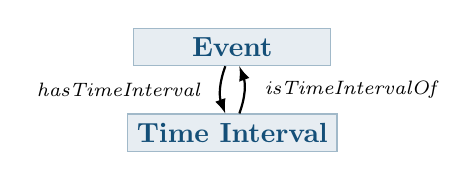
\begin{tikzpicture}
	    \node[owlclass] (A) {Event};
	    \node[owlclass,below=0.6cm of A] (B) {Time Interval};
	    \draw (A) edge[relationxl] node[midway,label=left:hasTimeInterval] {} (B);
	    \draw (B) edge[relationxr] node[midway,label=right:isTimeIntervalOf] {} (A);
	\end{tikzpicture}}
	%% Example KnowRob language expressions
	\ODPEXAMPLES{
		\emph{occurs($x$)} &
		$x$ is an occurence \\
		% % % % %
		\emph{is\_time\_interval($x$)} &
		$x$ is a time interval \\
		% % % % %
		\emph{has\_time\_interval($y$,$x$)} &
		$x$ is the time interval of event $y$
	}
\end{ODP}

\begin{ODP}{Occurences2}
	\ODPINTENT{To quantify when something has happened.}
	\ODPDEFINEDIN{SOMA.owl}
	\ODPQUESTION{When did it happen?}
	\ODPGRAPHIC{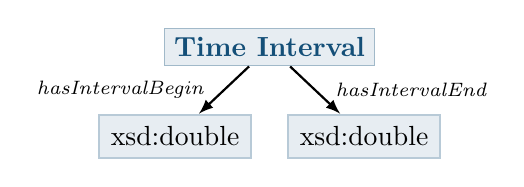
\begin{tikzpicture}
	    \node[owlclass] (TI) {Time Interval};
	    \node[data,below=0.6cm of TI,xshift=-1.2cm] (BEGIN) {xsd:double};
	    \node[data,below=0.6cm of TI,xshift=1.2cm] (END) {xsd:double};
	    \draw (TI)  edge[relation] node[midway,label=left:hasIntervalBegin] {} (BEGIN);
	    \draw (TI)  edge[relation] node[midway,label=right:hasIntervalEnd] {} (END);
	\end{tikzpicture}}
	%% Example KnowRob language expressions
	\ODPEXAMPLES{
		\emph{occurs($x$) during [$y$,$z$]} &
		$x$ occurs between the occurrences of $y$ and $z$ \\
		% % % % %
		\emph{occurs($x$) since $y$} &
		$x$ and $y$ begin at the same time \\
		% % % % %
		\emph{occurs($x$) until $y$} &
		$x$ and $y$ end at the same time
	}
\end{ODP}

% % % % % % % % % % % % % % % % %
% % % % % % % % % % % % % % % % %
\subsubsection{Participation}
\label{sec:participation}
%% Summary of Figure below
Events always involve some objects that play a certain role during the event. The role of being the \emph{patient} of some event being an example. This is that the event is directed towards the object. It is not always directly observable what the role of an object might be, however, it is less problematic to just state that the object \emph{has participated} in some event without naming a role.

\begin{ODP}{Participation}
	\ODPINTENT{To represent participation of an object in an event.}
	\ODPDEFINEDIN{DUL.owl}
	\ODPQUESTION{Which objects do participate in this event? In which events does this object participate in?}
	\ODPGRAPHIC{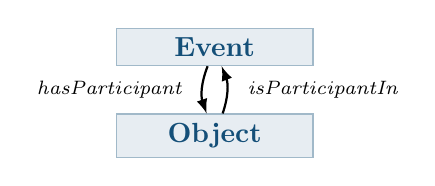
\begin{tikzpicture}
	    \node[owlclass] (A) {Event};
	    \node[owlclass,below=0.6cm of A] (B) {Object};
	    \draw (A) edge[relationxl] node[midway,label=left:hasParticipant] {} (B);
	    \draw (B) edge[relationxr] node[midway,label=right:isParticipantIn] {} (A);
	\end{tikzpicture}}
	%% Example KnowRob language expressions
	\ODPEXAMPLES{
		\emph{has\_participant($x$,$y$)} &
		$y$ is involved in event $x$
	}
\end{ODP}

%\textbf{todo: Sascha write this}
Agents are defined as \emph{agentive objects, either physical (e.g. a robot, a human or a whale) or social (e.g. a corporation, an institution or a community)}, Actions are defined as events with \emph{at least one agent that is participating in it, and that is executing a task}. An example would be an robot that is grasping an object. In that case the robot is the agent and grasping would be the a task executed in an action. Actions can be executed by multiple agents. 

\begin{ODP}{Action Execution}
	\ODPINTENT{To represent that an agent has executed an action.}
	\ODPDEFINEDIN{SOMA.owl}
	\ODPQUESTION{Which agent did execute this action? Which actions are executed by this agent?}
	\ODPGRAPHIC{
	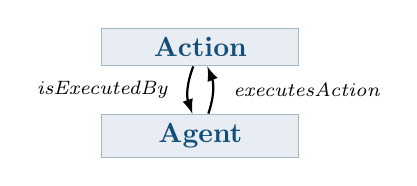
\begin{tikzpicture}
	    \node[owlclass] (A) {Action};
	    \node[owlclass,below=0.6cm of A] (B) {Agent};
	    \draw (A) edge[relationxl] node[midway,label=left:isExecutedBy] {} (B);
	    \draw (B) edge[relationxr] node[midway,label=right:executesAction] {} (A);
	\end{tikzpicture}
	}
	%% Example KnowRob language expressions
	\ODPEXAMPLES{
		\emph{is\_executed\_by($x$,$y$)} &
		$y$ is executed by $x$
	}
\end{ODP}

% % % % % % % % % % % % % % % % %
% % % % % % % % % % % % % % % % %
\subsubsection{Composition}
\label{sec:composition}

%\textbf{todo: Mihai write this.}
%\textbf{todo: why isn't hasPhase Event-to-Event?}

Because an Entity \todo{Seba: What is an Entity ? Is this an object?} often has relevant internal structure, it is necessary to represent relations between it and the other entities that make up its composition. DUL provides two such structuring relations: \emph{hasConstituent} and \emph{hasPart}. We will focus on \emph{hasPart} in this section, but we will briefly discuss the difference between the two relations as well. \todo{Seba: Why only hasPart ?}

The \emph{hasConstituent} relation is intended to connect entities from different ontological layers or levels of abstraction of looking at the world. A material is a constituent of the object it makes up; individual persons are constituents of a corporation. While these constituency relations could often be in colloquial language described as parthood, DUL reserves parthood for more restrictive connections between entities closer to each other in their ontological characterization. For example, a corporation is a \emph{SocialObject} and as such can only have \emph{SocialObjects} as parts, whereas human persons are \emph{PhysicalAgents}, disjoint from \emph{SocialObjects}.

The \emph{hasPart} relation is transitive and defined to have domain and range \emph{Entity}, that is, in principle it could link entities from any concepts together. However, various concepts restrict what can be parts of their instances as exemplified above; as another example, \emph{PhysicalObjects} can only have other \emph{PhysicalObjects} as parts. In SOMA, we define more specialized subproperties of \emph{hasPart} to deal with parts of \emph{Events} vs. parts of \emph{Objects}. The relevant properties are \emph{hasPhase} and \emph{hasComponent} respectively; both are subproperties of \emph{hasPart}.

\begin{ODP}{Event Phases}
	\ODPINTENT{To represent how an event is composed of phases.}
	\ODPDEFINEDIN{SOMA.owl}
	\ODPQUESTION{What are the phases of this action? Is this a phase of some action?}
	\ODPGRAPHIC{
	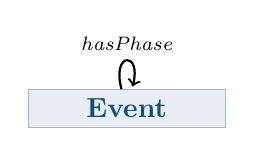
\begin{tikzpicture}
	    \node[owlclass] (E) {Event};
	    \path (E) edge[relation,loop above] node {hasPhase} (E);
	\end{tikzpicture}
	}
	%% Example KnowRob language expressions
	\ODPEXAMPLES{
		\emph{has\_phase($x$,$y$)} &
		$y$ is a phase of $x$
	}
\end{ODP}

%\lipsum[2]

\begin{ODP}{Composition}
	\ODPINTENT{To represent proper parthood of objects.}
	\ODPDEFINEDIN{DUL.owl}
	\ODPQUESTION{What is this object component of? What are the components of this object?}
	\ODPGRAPHIC{
	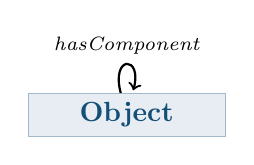
\begin{tikzpicture}
	    \node[owlclass] (E) {Object};
	    \path (E) edge[relation,loop above] node {hasComponent} (E);
	\end{tikzpicture}
	}
	%% Example KnowRob language expressions
	\ODPEXAMPLES{
		\emph{has\_component($x$,$y$)} &
		$y$ is a proper part of $x$
	}
\end{ODP}

\todo{Seba: For me this section makes sense. However, I have the feeling that compared to the previous sections, this section requires maybe more knowledge in ontologies to be understand. Maybe we should give it to someone how does not have any knowledge about ontologies.}

\todo{Daniel: I agree, probably we do not need to discuss the distinction between hasConstituent and hasPart here as it does not help the people to generate neems. We should limit to what is necessary here.}

% % % % % % % % % % % % % % % % %
% % % % % % % % % % % % % % % % %
\subsubsection{Conceptual Classification}
\label{sec:classification}

The classification of entities is done from multiple viewpoints.
The most essential one is \emph{what the entitiy really is}.
This is reflected in the taxonomy.
However, entities may further be classified according to social aspects such as intention, purpose, etc.
This type of classification is based on the \emph{conceptualization} of entities.
In particular, conceptualizations of objects and events are used to classify them in the scope of some activity.
For this purpose,
a comprehensive collection of concepts is used to classify objects and events from a conceptual viewpoint (\textbf{todo: insert link to list of all concepts}).

An object that participates in an event usually plays a certain role during the event.
Some objects are designed to be used in certain ways, thus playing certain roles in specific tasks.
This is, for example, a box which is designed to be used as a container to store items.
However, roles may also be taken by objects that are not designed to be used as such.
The box could, for example, also be used as a door stopper, but surely it would be
inappropriate to classify it as such taxonomically.
Instead, roles are defined as concepts that are used to classify the objects that particpate in an event from a conceptual viewpoint.

\begin{ODP}{Object Role}
	\ODPINTENT{To represents objects and the roles they play.}
	\ODPDEFINEDIN{DUL.owl}
	\ODPQUESTION{What role does this object play? Which objects do play that role?}
	\ODPGRAPHIC{
	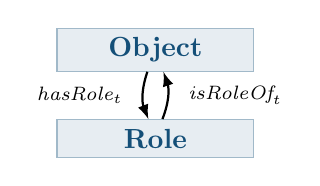
\begin{tikzpicture}
	    \node[owlclass] (A) {Object};
	    \node[owlclass,below=0.6cm of A] (B) {Role};
	    \draw (A) edge[relationxl] node[midway,label=left:$\text{hasRole}_t$] {} (B);
	    \draw (B) edge[relationxr] node[midway,label=right:$\text{isRoleOf}_t$] {} (A);
	\end{tikzpicture}
	}
	%% Example KnowRob language expressions
	\ODPEXAMPLES{
		\emph{has\_role($x$,$y$)} &
		$y$ is a role of $x$ \\
		% % % % %
		\emph{has\_role($x$,$y$) during $z$} &
		$y$ is a role of $x$ during the occurrence of $z$
	}
\end{ODP}

The conceptualization of an event is about how it should be interpreted, executed, expected, seen, etc.
One aspect is that a single event may contribute to multiple goals, such as when an ingredient is fetched that is partly used in a step of a cooking recipe, and partly eaten raw to satisfy hunger.
In such a case, the taxonomical category of the event would be unclear in case it should describe the goal to which the event contributes.
Another aspect is that intentions of agents may not always be known such that the classification of events based on their goals is difficult, and different viewpoints on the same event may exist.
Hence, when referring to goals, intentions, etc. we rather employ conceptual classification.
This allows us to represent several different classifications of the same event in one or more situational contexts, for example an interpretations of the same event from different viewpoints.
%\todo{Seba: How the conceptualization of an event looks in the end? Do we have only one classification or can it have multiple classifications if the goal is not clear?}

\begin{ODP}{??}
	\ODPINTENT{To represent how events should be interpreted, executed, expected, seen, etc.}
	\ODPDEFINEDIN{SOMA.owl}
	\ODPQUESTION{What are the events that are classified by this concept? What are the concepts that classify this event?}
	\ODPGRAPHIC{
	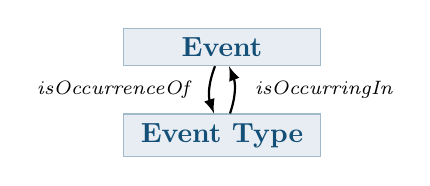
\begin{tikzpicture}
	    \node[owlclass] (A) {Event};
	    \node[owlclass,below=0.6cm of A] (B) {Event Type};
	    \draw (A) edge[relationxl] node[midway,label=left:isOccurrenceOf] {} (B);
	    \draw (B) edge[relationxr] node[midway,label=right:isOccurringIn] {} (A);
	\end{tikzpicture}
	}
	%% Example KnowRob language expressions
	\ODPEXAMPLES{
		\emph{is\_occurring\_in($x$,$y$)} &
		$y$ is an occurrence that is classified by $x$ \\
		% % % % %
		\emph{is\_executed\_in($x$,$y$)} &
		$y$ is an action that executes the task $x$
	}
\end{ODP}

%This ODP allows to make assertions on roles played by agents without involving the agents that play that roles, and vice versa. It allows to express neither the context type in which tasks are defined, not the particular context in which the action is carried out. Moreover, it does not allow to express the time at which the task is executed through the action (for actions that do not solely execute that certain task).
%\lipsum[2]

%\begin{ODP}{Task Execution}
%	\ODPINTENT{To represent actions through which tasks are executed.}
%	\ODPDEFINEDIN{DUL.owl}
%	\ODPQUESTION{Which task is executed through this action? What actions could execute that task?}
%	\ODPGRAPHIC{
%	\begin{tikzpicture}
%	    \node[owlclass] (A) {Action};
%	    \node[owlclass,below=0.6cm of EVT] (B) {Task};
%	    \draw (A) edge[relationxl] node[midway,label=left:executesTask] {} (B);
%	    \draw (B) edge[relationxr] node[midway,label=right:isExecutedIn] {} (A);
%	\end{tikzpicture}
%	}
%	%% Example KnowRob language expressions
%	\ODPEXAMPLES{
%		\emph{??} &
%		??
%	}
%\end{ODP}

% % % % % % % % % % % % % % % % %
% % % % % % % % % % % % % % % % %
\subsubsection{Object Transformation}
\label{sec:transformation}

Objects typically undergo changes by taking part in actions or processes. Such changes typically take one of two forms: either some property of an object changes value, or the object itself modifies its ontological characterization. As an example, a wad of dough being transported from the table to the inside of an oven has changed its position, but is still, at this point, a wad of dough. Left in a hot oven for enough time however, the wad of dough becomes bread.

The variation with time of object qualities has been described in section~\ref{sec:qualification}. The object transformation pattern, described here, handles the changes of an object's ontological classification through time. An immediate problem is that ontological characterizations are necessarily discrete -- there is a finite number of classes an object can belong to -- while change in the physical world is continuous. In the example above, the wad of dough ceases to be dough after a few moments in the oven, because its chemical composition is changing away from the composition of dough. Nonetheless, it is not bread yet.

For practical purposes however, human beings often do not care about the exact classification of an object undergoing ontological change; only the endpoints are important. Also, there is a tendency to loosely apply ontological classification to the changing object, as if it were on either side of the transformation. The cooking wad of dough could be referred to as dough, or it could be referred to as bread. It is both, and neither. While sufficient for causal discourse, such carelessness would not work in a formal system. Hence, the approach in SOMA is to define a class of objects called \emph{Transient}, and it is to this class that objects undergoing ontological classification change belong to. A Transient \emph{transitionsFrom} some object with a specific classification (e.g. \emph{Dough}) and \emph{transitionsTo} another object with a specific classification (e.g. \emph{Bread}). These two relations can be combined into the \emph{transitionsBack} relation, to cover situations where an object changes in essential ways during an event, but returns to being itself after the event completes, such as a catalyst in a chemical reaction.
 
% This pattern addresses the fact that objects change by undergoing/taking part in Processes. For example, the PancakeMix becomes, through Baking, a Pancake. However, the ontological status of the object while the process takes place is unclear: the object placed on the frying pan is not a Pancake until Baking finishes, but it's not PancakeMix either once it begins to coagulate. In the EASE approach, the object in-between such characterizations is a Transient. A Transient transitionsFrom an Object, and possibly transitionsTo an Object. It may also be the case that a Transient transitionsBack to an Object, to indicate that once the process completes, the same Object is restored; this would be the case for example for catalysts in chemistry, or a loaf of bread after slicing, if there is enough bread left.
%\lipsum[2]

\begin{ODP}{Transient}
	\ODPINTENT{Ontological classification for objects undergoing type changes.}
	\ODPDEFINEDIN{SOMA.owl}
	\ODPQUESTION{What sort of object is this? What objects ``went'' into the making of another? What is the outcome of some process of change acting on an object? Does an object preserve or restore its identity after change?}
	\ODPGRAPHIC{
	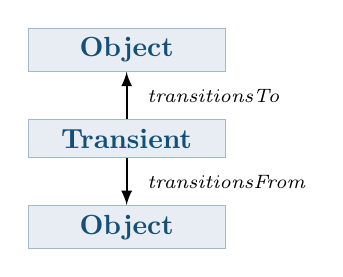
\begin{tikzpicture}
 %\node[owlclass] (TRANSIENT) {
 %\begin{owlclass}{Transient}
 % \item \texttt{Object}
 % \item $(\exists\emph{transitionsFrom}.\texttt{Object})$
 % \item $(\forall\emph{transitionsTo}.\texttt{Object})$
 %\end{owlclass}
 %};
 %\node[owlclass,below=0.6cm of TRANSIENT] (TRANSITIONSBACK) {
 %\begin{owlclass}{transitionsBack}
 % \item \texttt{transitionsFrom}
 % \item \texttt{transitionsTo}
 %\end{owlclass}
 %};
	    \node[owlclass] (A) {Transient};
	    \node[owlclass,below=0.6cm of A] (B) {Object};
	    \node[owlclass,above=0.6cm of A] (C) {Object};
	    \draw (A) edge[relation] node[midway,label=right:transitionsFrom] {} (B);
	    \draw (A) edge[relation] node[midway,label=right:transitionsTo] {} (C);
	\end{tikzpicture}
	}
	%% Example KnowRob language expressions
	\ODPEXAMPLES{
		\emph{transitionsFrom('A','B')} & By entering some process of change, object 'B' becomes Transient object 'A'.\\
		\emph{transitionsTo('A','B')} & By completing some process of change, transient 'A' becomes object 'B'.\\
		\emph{transitionsBack('A','B')} & Object 'B' entered some process of change during which its ontological classification is unclear and it is replaced by Transient 'A', but after the process completes object 'B' is restored.\\
	}
\end{ODP}

% % % % % % % % % % % % % % % % %
% % % % % % % % % % % % % % % % %
\subsubsection{Force Interaction}

\textbf{todo: Daniel write this}
\textbf{todo: preservative vs. alterative interaction}
\textbf{todo: how to represent who is stronger? can measured forces be included in the NEEM?}
\textbf{todo: isProcessTypeOf relation is not nice}
\lipsum[2]

\begin{ODP}{?}
	\ODPINTENT{To represent force dynamical event characteristics.}
	\ODPDEFINEDIN{SOMA.owl}
	\ODPQUESTION{What entity is the agonist in this event? What are the events where this entity is an antagonist? Which entity is stronger in this event? What is the force dynamical tendency in this event?}
	\ODPGRAPHIC{
	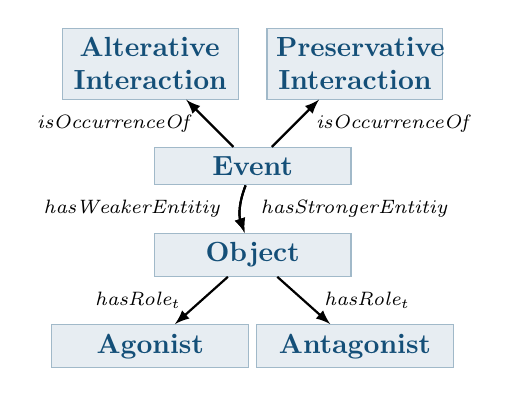
\begin{tikzpicture}
	    \node[owlclass] (A) {Event};
	    \node[owlclass,below=0.6cm of A] (B) {Object};
	    \node[owlclass,below=0.6cm of B,xshift=-1.3cm] (C) {Agonist};
	    \node[owlclass,below=0.6cm of B,xshift=1.3cm]  (D) {Antagonist};
	    \node[owlclass_f,above=0.6cm of A,xshift=-1.3cm] (E) {Alterative Interaction};
	    \node[owlclass_f,above=0.6cm of A,xshift=1.3cm]  (F) {Preservative Interaction};
	    \draw (B) edge[relation] node[midway,label=left:$\text{hasRole}_t$] {} (C);
	    \draw (B) edge[relation] node[midway,label=right:$\text{hasRole}_t$] {} (D);
	    \draw (A) edge[relation] node[midway,label=left:$\text{isOccurrenceOf}$] {} (E);
	    \draw (A) edge[relation] node[midway,label=right:$\text{isOccurrenceOf}$] {} (F);
	    \draw (A) edge[relationxl] node[midway,label=left:hasWeakerEntitiy] {} (B);
	    \draw (A) edge[relationxr] node[midway,label=right:hasStrongerEntitiy] {} (B);
	\end{tikzpicture}
	}
	%% Example KnowRob language expressions
	\ODPEXAMPLES{
		\emph{??} & ??
	}
\end{ODP}

\lipsum[2]

\begin{ODP}{?}
	\ODPINTENT{To quantify force dynamical event characteristics.}
	\ODPDEFINEDIN{SOMA.owl}
	\ODPQUESTION{What is the effort of the agonist in this event?}
	\ODPGRAPHIC{
	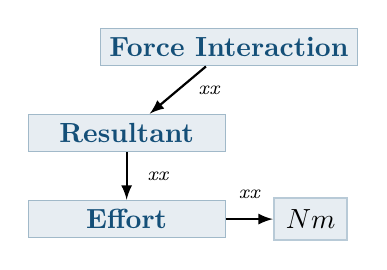
\begin{tikzpicture}
	    \node[owlclass] (B) {Force Interaction};
	    \node[owlclass,below=0.6cm of B,xshift=-1.3cm] (C) {Resultant};
	    \node[owlclass,below=0.6cm of C] (D) {Effort};
	    \node[data,right=0.6cm of D] (E) {$Nm$};
	    \draw (B) edge[relation] node[midway,label=right:xx] {} (C);
	    \draw (C) edge[relation] node[midway,label=right:xx] {} (D);
	    \draw (D) edge[relation] node[midway,label=above:xx] {} (E);
	\end{tikzpicture}
	}
	%% Example KnowRob language expressions
	\ODPEXAMPLES{
		\emph{??} & ??
	}
\end{ODP}

% % % % % % % % % % % % % % % % %
% % % % % % % % % % % % % % % % %
\subsubsection{Episodes}
\label{sec:episodes}

An episode is seen as a \emph{relational context} created by an observer that creates a view on a set of entities such as actions that were perfomed, and objects that played a role. We say that an episode is a \emph{setting for} each entity that is relevant for the scope of the episode. As an example, consider the statement \emph{"this morning the robot made a mess on the floor while preparing coffee"}, where the preparation of coffee in the morning is the setting for the robot, the floor, and the actions that were perfomed.
Several specializations of the general \emph{is setting for} relation exist that can be used to distinguish between entities based on their type -- these are, among others, \emph{includesObject} and \emph{includesAgent}.
However, assuming hierachical organization of objects (i.e. all objects are part of some map), and events (i.e. an event is composed into sub-events) only those entities at the root of the composition (e.g. the map) are required to be included explicitely in the episode.

\begin{ODP}{isSettingFor}
	\ODPINTENT{To represent that entites are included in a situation.}
	\ODPDEFINEDIN{DUL.owl}
	\ODPQUESTION{What are the entities that are relevant for this situation? What are the situations where this entity is relevant?}
	\ODPGRAPHIC{
	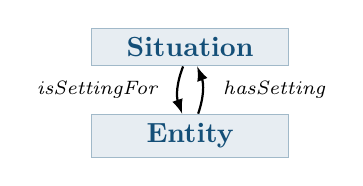
\begin{tikzpicture}
	    \node[owlclass] (A) {Situation};
	    \node[owlclass,below=0.6cm of A] (B) {Entity};
	    \draw (A) edge[relationxl] node[midway,label=left:isSettingFor] {} (B);
	    \draw (B) edge[relationxr] node[midway,label=right:hasSetting] {} (A);
	    hasSetting
	\end{tikzpicture}
	}
	%% Example KnowRob language expressions
	\ODPEXAMPLES{
		\emph{is\_setting\_for($x$,$y$)} &
		$x$ is a setting for $y$
	}
\end{ODP}

Episodes refer to concrete occurences with actual objects that are involved, and actual events that occur.
The conceptualization of an episode is an abstraction that refers to concepts instead that are used to classify entities that are included in the episode.
Such conceptualizations are called \emph{descriptions}.
We say that an episode \emph{satisfies} a description in case the view represented
by the episode is consistent with the conceptualization given by the description.
Diagnosis being one example of a description of an episode.
Stating that the performance of the robot was \emph{amateurish} when it made a mess on the floor while
preparing coffee is one example for describing an epsiode.
Another type of descriptions are plans that are used to conceptualize the structure of an activity.

\begin{ODP}{satisfies}
	\ODPINTENT{To represent a conceptualization of a situation.}
	\ODPDEFINEDIN{DUL.owl}
	\ODPQUESTION{How can this situation be conceptualized? What are the situations that are consitent with this conceptualization?}
	\ODPGRAPHIC{
	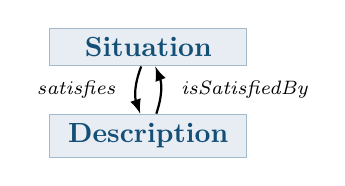
\begin{tikzpicture}
	    \node[owlclass] (A) {Situation};
	    \node[owlclass,below=0.6cm of A] (B) {Description};
	    \draw (A) edge[relationxl] node[midway,label=left:satisfies] {} (B);
	    \draw (B) edge[relationxr] node[midway,label=right:isSatisfiedBy] {} (A);
	\end{tikzpicture}
	}
	%% Example KnowRob language expressions
	\ODPEXAMPLES{
		\emph{satisfies($x$,$y$)} &
		$x$ is consistent with $y$
	}
\end{ODP}

% % % % % % % % % % % % % % % % %
% % % % % % % % % % % % % % % % %
% % % % % % % % % % % % % % % % %
% % % % % % % % % % % % % % % % %
% % % % % % % % % % % % % % % % %
% % % % % % % % % % % % % % % % %

\iffalse
\begin{ODP}{Process vs. Action}
%\ODPDESCRIPTION{An Action is an Event with at least one Agent participant, such that this Agent has a Task, often defined by a Plan or Workflow, which it executes through the Action. A Process is an Event for which no such commitments have been made. In DUL, these classes are not disjoint, allowing a particular event individual to be classified as either, depending on whether we care to record an agent and its goals or not. In EASE, we use Process as a top-level class for events with no agentive participant.}
\ODPINTENT{To represent the intentional and agentive structure-- or lack thereof-- behind Events.}
\ODPDEFINEDIN{DUL.owl}
\ODPQUESTION{
  \emph{Is there anyone responsible for the event?}
  \emph{What are they trying to do?}
  \emph{How did an event unfold?}}
\ODPGRAPHIC{
\begin{tikzpicture}
 \node[owlclass] (ACTION) {
 \begin{owlclass}{Action}
  \item \texttt{Event}
  \item $(\exists \emph{hasParticipant}.\texttt{Agent})$
 \end{owlclass}
 };
 \node[owlclass,below=0.6cm of ACTION] (PROCESS) {
 \begin{owlclass}{Process}
  \item \texttt{Event}
 \end{owlclass}
 };
\end{tikzpicture}
}
\end{ODP}

\begin{ODP}{State, Configuration, Gestallt}
%\ODPDESCRIPTION{A state is a configuration of the world that is construed to be stable on its own. Outside disturbances may cause state transitions, and the settling into some other, self-stable configuration. A State is also characterized by a Description, that indicates things such as what kind of entities participate in the state, what relations might exist between them, what regions may be used by particular qualities of the participants. This Description is, in general, referred to as a Configuration, however some common examples are Goals-- describe desired states of the world--, Norms-- describe states that should be kept--, and Diagnoses-- describe a state that causes certain observable symptoms. States are classified by Gestallts. \textbf{TODO}: Generalize this and/or split it: classification by an event type and structuring by a description are different ODPs in the current list. All three event subclasses (Actions, Processes, States) now are each part of their own Event-Concept-Description triad, where the Concept classifies the Event, and the Description, by describing the classifying Concept, structures the Event.
}
\ODPINTENT{Ontological representation for situations in the world that are cognitively construed as stable arrangements of entities.}
\ODPDEFINEDIN{EASE-STATE.owl}
\ODPQUESTION{
  \emph{What are stable arrangements?}
  \emph{What is meant by ``state'' of the world?}
  \emph{What characterizes a state?}}
\emph{Examples}
%\begin{itemize}
%  \item AssemblyConnection: two objects are in a rigid connection, such that the movement of one determines the movement of the other. In this case the characterizing Configuration for this State uses several Roles-- one for each part/geometric feature belonging to the connected objects-- and puts constraints on the relative positioning of these geometric features such that they interlock to produce the rigid connection.
%  \item Contact: two objects are in mechanical contact. The characterizing Configuration uses two Roles, one for each participating object, and puts constraints on the Pose qualities of the participants: the poses should be such that the participants touch.
%  \item FunctionalControl: an object restricts the movement of another, at least partially. The Configuration uses the Roles Item and Restrictor. More concrete examples are Containment: the Restrictor is a Container, and the Pose quality of the Item should use the region inside the Container; and Support: both Restrictor and Item are objects, placed in such a way that the Item does not move because of gravity.
%  \item PhysicallyAccessible: the Configuration for this state uses the roles Item, a Container or Protector, and optionally an Accessor and a Task, and states that an Item is either placed in a Container or protected by a Protector, but the placement of the Item and Container is such that an Accessor may nevertheless reach the Item in order to perform a Task. For a more concrete example, a DoorOpen is a kind of PhysicallyAccessible where the Protector is a door, the Item is the inside of the room behind the door, the Accessor is some person and the Task is to walk into the inside of the room.
%\end{itemize}
\end{ODP}

\begin{ODP}{Designed Artifact}
%\ODPDESCRIPTION{A DesignedArtifact is a physical object described by a Design. In EASE, Designs refer to the form, but also the function of an object. This allows us to say that an object is ``for'' a particular purpose, even though it might be used for something else instead. For example, a cup is a BeverageContainer but can be used as a Flowerpot. Designs form a hierarchy of specificity, for example $DesignMilkContainer \sqsubseteq DesignBeverageContainer \sqsubseteq DesginContainer \sqsubseteq Design$. The justification for this pattern is that the type of an object is rigid, but the roles it plays in events change. A naive taxonomy, without a notion similar to Design, cannot tackle the fact that objects are usable in several ways beyond the obvious; a hammer isn't always a hammer, sometimes it's a paperweight. On the other hand, a usable ontology of objects must take into account how human users refer to objects by their default use.}
\ODPINTENT{To explicate the intuitive classification human users would have of objects, based on their default uses.}
\ODPDEFINEDIN{DUL.owl, EASE.owl, EASE-middle.owl}
\ODPQUESTION{
  \emph{What sort of object is this?}
  \emph{What is the intended use of the object?}
  \emph{How did an event unfold?}}
\ODPGRAPHIC{
\begin{tikzpicture}
 \node[owlclass] (DESIGNEDARTIFACT) {
 \begin{owlclass}{DesignedArtifact}
  \item \texttt{PhysicalArtifact}
  \item $(\exists\emph{isDescribedBy}.\texttt{Design})$
 \end{owlclass}
 };
 \node[owlclass,below=0.6cm of DESIGNEDARTIFACT] (DESIGN) {
 \begin{owlclass}{Design}
  \item \texttt{Description}
 \end{owlclass}
 };
 \draw (DESIGNEDARTIFACT) edge[thick,-,dashed,blue!60] (DESIGN);
\end{tikzpicture}
}
\end{ODP}
\fi

% In version \neemversion the \neemnar consists the belief state and action task hierarchy. 
% In the following sections we will describe how the belief state and action task hierarchy are represented.
% An concrete example for a logged \neemnar will be given in Chapter \ref{ch:example}.

% \subsection{Belief State}
% 
In EASE, we investigate everyday manipulation activities.
These involve the interaction with physical objects such as
grasping an object and putting it somewhere,
or taking a tool and applying it on an object to achieve a certain effect.
To tell a comprehensive story about its activity,
an agent needs to memorize the relation of action to
physical objects that are salient during the action.

One requirement for this is that beliefs of the agent about the existence
of physical objects must be maintained by the system.
In some cases, when the existence is known in advance,
it is sufficient to supply this knowledge to the agent through
a static ontology holding facts about existence of physical objects
in the environment of the agent.
This is, for example, useful to supply knowledge about a static
environment such as a kitchen with fixed set of appliances.
In more dynamic set-ups, however, the beliefs about the existence
of physical objects must be formed through specialized perception
methods, or through logical reasoning.
This is, for example, the case when the particular set of objects
contained in a drawer are unknown in advance.
We consider this type of information as part of the NEEM narrative
to keep these beliefs persistent, and to allow referring to
the perceived objects in action descriptions.

Episodic memories capture information about temporal situations
during which the beliefs of the agent evolve according to
perception, action, and logical inference.
NEEMs capture this evolution of beliefs.
As such, revised or false beliefs are not deleted but kept
persistently as part of the NEEM narrative.
This is to allow for deeper analysis of the agent performance,
and to provide richer input for learning algorithms.
This is realized through a 4D ontology that we describe at
the end of this section.

%%%%%%%%%%%%%%%%%%%%%%%%%%%%%
%%%%%%%%%%%%%%%%%%%%%%%%%%%%%
%%%%%%%%%%%%%%%%%%%%%%%%%%%%%
%%%%%%%%%%%%%%%%%%%%%%%%%%%%%
\subsection{Tangible Objects}
To refer to objects in action descriptions only the name of the 
object must be known to the NEEM acquisition system.
\knowrob comes with a rather comprehensive object type system,
with about XXX different object classes~\cite{knowrob-ontology}.
The type system is represented as part of the TBOX of the knowledge base.
Perceived objects are represented as instance of one of the object types
provided by the \knowrob system.
This type of information is part of the ABOX of the knowledge base.
The name of an object is usually the name of the class followed
by a underscore character and a 8-digit hash,
but could potentially be any unique name string.

\todo{introduce base class of objects, give some details about taxonomy}

In systems relying on sensor information and statistical models one has to deal
with the uncertainty coming from the use of these information sources.
This also affects beliefs about the identity of objects.
The problem of identity resolution can trivially be approached
by computing euclidean distance to known objects.
If the distance is below a certain threshold, it can often be assumed that it is the same object.
Background knowledge can be used to find better estimates for object identity:
An object is inside the gripper as long as it is grasped,
pulled down by gravity to the plane below when the grasp is released again,
and so forth.
Also, the identity of objects is often not so important for decision making,
but rather the properties of the object.
For successfully preparing a slice of bread, for example, any butter will do.
But if there are two butter packages and one is not yet opened one would rather
use the opened one to avoid it getting rancid.
When acquiring NEEMs one has to deal with this identity resolution problem
to allow for referring to objects in the narrative part of the episodic memory.

In the remainder of this section we describe the fundamental binary predicates to
describe physical objects in the belief state.

\begin{description}
\item[\textbf{rdf:type}] 
The most fundamental assertion about an object next to its name is its type.
Types are asserted through the \emph{rdf:type}
property with one of the object types as value.
Ontologies are subsumption hierarchies that derive 
knowledge about more specific concepts from more general concepts.
This allows, for example, to describe the relation between object and action
on a general level that applies to a larger class of objects and actions.
It is further possible to assert multiple types from different branches
of the type hierarchy for a single object.
For example, some mobile phone may also be used as projector while other mobile phones,
without the projector hardware, should not be classified as projector.
%%%%%%%%%%%%%%%%%%%%%%%%%%%%%
%%%%%%%%%%%%%%%%%%%%%%%%%%%%%
\item[\textbf{physicalParts}]
$Whole\ \emph{physicalParts}\ Part$ means
that $Part$ is tangible and one of the distinct parts of the
more complex tangible object $Whole$.
Manipulation is often about putting together parts to form a bigger whole.
During table setting, for example, objects are arranged such that they form
place settings for the different participants.
The objects are placed intentionally such that humans can easily reach them from their seat,
see which objects belong to which place setting, and infer what objects belong to whom.
Another example are assembly tasks during which an agent tries
to put together some mechanical parts using screwing connections, snap-in connection,
and so on to create an assembled product from scattered pieces available.
NEEMs can also represent this partonomy information through dedicated predicates
linking parts to the bigger whole.
In particular, the \ease ontology defines the following sub-properties of \emph{physicalParts}:
\emph{dangerousParts} (e.g., the blade of a knife),
\emph{electricalParts} (i.e., parts that need electrical current to work),
\emph{mealComponents} (i.e., the ingredients of a meal).
%%%%%%%%%%%%%%%%%%%%%%%%%%%%%
%%%%%%%%%%%%%%%%%%%%%%%%%%%%%
\item[\textbf{frameName}] \dots
\end{description}

\todo{some other relevant predicates? shape, color, mesh, pose?}

%%%%%%%%%%%%%%%%%%%%%%%%%%%%%
%%%%%%%%%%%%%%%%%%%%%%%%%%%%%
%%%%%%%%%%%%%%%%%%%%%%%%%%%%%
%%%%%%%%%%%%%%%%%%%%%%%%%%%%%
\subsection{Kinematic Objects}
\begin{enumerate}
 \item \todo{object parts can be connected through joints}
 \item \todo{what types of joints exist?}
 \item \todo{what predicates can be used to describe them?}
\end{enumerate}

%%%%%%%%%%%%%%%%%%%%%%%%%%%%%
%%%%%%%%%%%%%%%%%%%%%%%%%%%%%
%%%%%%%%%%%%%%%%%%%%%%%%%%%%%
%%%%%%%%%%%%%%%%%%%%%%%%%%%%%
\subsection{Environment Maps}
Semantic maps are detailed representations of the environment of some agent.
These include geometrical and visual information about objects and appliances,
their functional decomposition, and their state.
Modern game engines reach an impressive level of detail, with individual
leaves falling down trees, etc.
In EASE, we try to reach this level of detail in our semantic map representations.
We do this to provide very comprehensive information about situated experiences
from which general knowledge can be learned.
We believe that this high level of detail will allow us to learn more robust
models and with less training data then would be possible with
a more abstracted representation of environments.

The \emph{SemanticMap} itself could be a \emph{Room}, a \emph{Building}, or some other type of connected
region in which some agent can do navigation and manipulation.
The ontology defines some more specific room classes including
\emph{Kitchen}, \emph{LivingRoom} and \emph{StoreRoom}.
This is useful, for example, to correlate objects with their likely storage room,
or to relate the rooms with common activities performed in them.

\begin{description}
%%%%%%%%%%%%%%%%%%%%%%%%%%%%%
%%%%%%%%%%%%%%%%%%%%%%%%%%%%%
\item[\textbf{describedInMap}]
$Object\ \emph{describedInMap}\ Map$ means \dots
\end{description}

\todo{also describe how rooms relate to buildings, etc.?}
\todo{something about the state?}


\subsection{Temporal Representation}
\dots

% \subsection{Action Hierarchy}
% \label{ch:narrative,sec:actionHierarchy}
% In this section, we will describe how an action task hierarchy is represented in the \neemnar. 
% Since we are using \cram on our robots our plans do not necessary generate a sequence of actions, instead they will generate rather an hierarchy of actions.
% During the plan execution we are logging all executed actions with its parameters and represent the hierarchy in \owl.
% The general idea of the model is that an action will be represented as an individual of the class \owlClass{knowrob:'Action'}.
% This individual can be a direct instance of the class \owlClass{knowrob:'Action'} or its subclass.
% \todo{Add all supported action sub classes}
% With the predicates \owlPredicate{subAction}, \owlPredicate{previousAction} and \owlPredicate{nextAction}, which all have as subject and object the type \owlClass{knowrob:'Action'}, we are able to represent the action hierarchy.
% In our understanding an logged action hierarchy in an \owl represents all actions which were executed during an experiment.
% Meaning, if we would extracted all actions from the \owl file and recreated the action tree, we would be able to analyze and reasoning about all executed actions during one specific experiment.

% In the next subsections we will describe the predicates and classes which we currently defined in the version \neemversion to log the actions which were executed by the robot during an experiment. 

% \subsection{Action Predicates}
% Every individual of the class \owlClass{knowrob:'Action'} class or its subclass which will be logged in the \owl file can be asserted with the following predicates (see Table \ref{table:action_task_predicates}).
% Some predicates in the table are marked as required.
% This means that if you are intending to upload your \owl file to \openease, every \owlClass{knowrob:'Action'} individual has to have the required properties asserted.
% %Otherwise the \owl file will be revoked from the server.\todo{We have to implement such checking in \openease.}
% The \openease server checks also if the objects of the predicates are associated with the correct class.

% \begin{table}[H]
% 	\begin{tabular}{| c | c | c | c |}
% 		\hline			
% 		\textbf{Subject} & \textbf{Predicate} & \textbf{Object}  & \textbf{Required} \\
% 		\hline
% 		Action & taskSuccess & xsd:boolean & Yes \\
% 		\hline
% 		Action & startTime & Timepoint & Yes \\
% 		\hline
% 		Action & endTime & Timepoint  & Yes \\
% 		\hline
% 		Action & subAction & Action & No \\
% 		\hline
% 		Action & nextAction & Action & No \\
% 		\hline
% 		Action & previousAction & Action & No \\
% 		\hline
% 	\end{tabular}
% 	\caption{Action Predicates}
% 	\label{table:action_task_predicates}
% \end{table}

% \begin{description}
% 	\item[\textbf{taskSuccess}] 
% 		This predicates points to data type \owlClass{xsd:boolean}.
% 		The value \textbf{true} represents that the action was executed successfully.
% 		If any errors occurred during the action execution, the data type will be set to \textbf{false}.
% 		\footnote{In the NEEM version \neemversion we do not log the exact error which happened during action.}
% 	\item[\textbf{startTime}]
% 		The \owlPredicate{startTime} represents when the action started.
% 		Instead of representing the startTime as a data point, we are creating an instance of the class \owlClass{Timepoint}.
% 		The implemenation is done in that way because it made writing prolog queries much more convenient. 
% 		The name of the individual is representing the exact time when the action started e.g.\ \textit{timepoint\_1523878415038090} which can be understood that the action started 1523878415038090 microseconds after 00:00:00 UTC, Thursday, 1 January 1970.
% 		We are using the Unix time to represent a time point \cite{matthew2011beginning}.
% 		However, we are considering to measure the time in microseconds.
% 		The reason for this decision is that we also want to create NEEMs in simulation.
% 		However, tasks in simulation can be executed so fast that logging in microseconds allowed to measure the performance of the task executions.
% 		Also the measurement in microseconds allowed to differentiate the running time between tasks.
% 	\item[\textbf{endTime}] 
% 		This predicate represents when the action ended.
% 		More information about how we log time points is described in the predicate description \owlPredicate{startTime}.
% 	\item[\textbf{subAction}]
% 		The predicate \owlPredicate{subAction} allows to create parent-child relation between two tasks. In the context of this predicate, the subject is the parent action and the object is the child action.
% 		It is possible that an \owlClass{Action} instance can have multiple \owlPredicate{subAction} predicates which point each to a single child action.
% 	\item[\textbf{nextAction}]
% 		To be able to create an sequential order of actions which where executed on the same hierarchy level, we defined the \owlPredicate{nextAction} predicate.
% 		The subject represents the action which was started first and points to the next sibling actions.
% 		\footnote{In the NEEM version \neemversion we are not differentiate if actions were executed in sequence or in parallel.}
% 	\item[\textbf{previousAction}]
% 		Like in \owlPredicate{previousAction} this predicate is created to create an sequential order between siblings tasks.
% 		However in this case, \owlPredicate{previousAction} connects an \owlClass{Action} instance with the sibling action which was performed previously.
% \end{description}


% \subsection{Action Parameter Predicates}
% 	\label{sec:actionParameterPredicactes}
% 	In general, actions have to have parameters which have to be asserted.
% 	Based on those assertions \cram is able to infer how to perform the task.
% 	For instance, a grasping task will be executed differently when the target object is a spoon compared to when the target object is a bottle.
% 	To understand the logged behavior of the robot better, we are logging to each action the corresponding parameters.
% 	For \cram we are using for our actions a set of predefined parameters.
% 	For example, when an action requires an object every \cram action has parameter name \textit{object} asserted.
% 	During the logging process, we are creating based on the parameter's value an instance of the class \owlClass{Object} and connect this instance with the \owlPredicate{objectActedOn}.
% 	\todo{Ref to belief state when object description is done}
% 	This implementation allows us to use the logger for new actions without the need to extend the logger.
% 	As long the \cram actions will use the predefined parameter names all parameters will be logged without the need to extend the logger.
% 	All predefined parameters are represented by a separated predicates which point to the parameter value which is an individual of the corresponding \owl class.
% 	Table \ref{table:action_parameter_predicates} shows the current parameter predicates which are supported by our NEEM representation.
% 	The design of the action parameter predicates is based on the work with our \pr.
% 	Therefore in the NEEM \neemversion it might be possible that the action parameters cannot be used by everyone in this state.
	 
% \begin{table}[H]
% \begin{tabular}{| c | c | c |}
% 	\hline			
% 	\textbf{Subject} & \textbf{Predicate} & \textbf{Object} \\
% 	\hline			
% 	Action & effort & qudt\#NewtonMeter \\
% 	\hline
%     Action & position & Float \\
%     \hline
% 	Action & arm & Pr2\#Pr2RightArm \\
% 	\hline
% 	Action & bodyPartsUsed & Pr2\#Pr2RightGripper \\
% 	\hline
% 	Action & goalLocation & Pose or Connected Space Region \\
% 	\hline
%     Action & objectActedOn & Object \\
% 	\hline
% 	Action & objectType & Object \\
% 	\hline
% \end{tabular}
% 	\caption{Action Parameter Predicates}
% 	\label{table:action_parameter_predicates}
% \end{table}

% \begin{description}
% 	\item[\textbf{effort}] 
% 		Effort is the grasping force in newton-meters.
% 		To model this we are using the \qudt ontology \footnote{http://qudt.org/}.
% 	\item[\textbf{position}]
% 		We are using this predicate to log the the goal position for the gripper of the \pr.
% 		The \pr accepts a joint angle in RAD to position its gripper.
% 		We decided to use a float data type to model the position to be able to represent more different types of position.
% 		For instance, our \boxy robot uses centimeters to position the gripper.
% 		Therefore with a float representation we are able to log from both robots the position parameter.
% 	\item[\textbf{arm}]
% 		With this predicate we want to log which arm was used to by the robot.
% 		The predicate points to an instance of the specific robot arm class.
% 		For instance, to model that the \pr used a right arm to grasp a bottle we are asserting the \owlPredicate{arm} predicate to an individual of the class \owlClass{Pr2RightArm}\footnote{http://knowrob.org/kb/PR2.owl}.
% 	\item[\textbf{bodyPartsUsed}]
% 		The \owlPredicate{bodyPartsUsed} predicate should represent which body part from the robot was used to perform the task.
% 		This predicate can be used \eg to represent that a gripper was used to perform the task.
% 		Like in \dots we also want to represent the body part as instance of the class which represents the body part.
% 	\item[\textbf{goalLocation}]
% 		This predicate can be used to represent the target or location parameter of an action.
% 		This predicate is suitable to represent \eg the target location of an \textit{Going} action.
% 		We are considering to different object types to log the goal location.
% 		Since our robots are build on \ros our robots can work with \textit{Poses} \footnote{http://docs.ros.org/api/geometry\_msgs/html/msg/Pose.html}.
% 		How we represent this \owl class is stated out in section \ref{sec:pose}.
		
% 		Since we are also using \cram, our robots can also encounter \textit{location designator} as goal locations\cite{beetz2010cram}.
% 		That means \cram can handle tasks like "Go to the kitchen counter".
% 		Since locations designators are more abstract we use the \owl class \owlClass{Connected Space Region} to log them.
% 		A more detailed description is given in section \ref{sec:connectedSpaceRegion}.
		
% 	\item[\textbf{objectActedOn}]
% 		With the predicate \owlClass{objectActedOn} we want to log which objects are given as parameter to the action.
% 		For instance, we can log which objects the robots looked for during a perception task and what objects he tried to grab.
% 	\item[\textbf{objectType}]
% 		The difference of \owlPredicate{objectType} compared to \owlPredicate{objectActedOn} is that \owlPredicate{objectType} define not a specific object but rather an object in general.
% 		For instance, if the robotic agent will get a task such as "grab the milk from the fridge".
% 		Given the task, the agent knows only that it has to grab a object of the type of milk from the fridge.
% 		So at this moment the robot does not know if the a milk box is actually in the fridge.
% 		Thereofre it has to recognize the milk first.
% 		If this was sucessfull then the robot will assoicated the following task the milk ID with the predicate \owlPredicate{objectActedOn} which the object will be the link to the speicifc object in the belieft state.
% \end{description}

% \subsection{Action Parameter Classes}
% As shown in section \ref{sec:actionParameterPredicactes} we are not only using data types to log the action parameter.
% In this section we are describing the \owl classes which we introduced to be able to log all parameters which we required to log during our experiments.

% \subsubsection{Pose}
% 	\label{sec:pose}
% 	This class is used to log coordinates given as parameter.
% 	Since our robots are using \ros we are logging poses.
% 	A pose consists from a Quaternion and a 3D vector.
% 	Since both together can only describe a Pose, both entities are required to be logged.
% 	\begin{table}[H]
% 		\begin{tabular}{| c | c | c | c |}
% 			\hline			
% 			\textbf{Subject} & \textbf{Predicate} & \textbf{Object} & \textbf{Required}\\
% 			\hline
% 			Pose & quaternion & String & Yes \\
% 			\hline
% 			Pose & translation & String & Yes \\			
% 			\hline
% 		\end{tabular}
% 		\caption{Pose Predicates}
% 		\label{table:pose_predicates}
% 	\end{table}
	
% 	\begin{description}
% 		\item[Quaternion] 
% 			%Quaternions are used to describe rotations in a three dimensionally space. \todo{Set reference to a Quaternions description}
% 			In the NEEM version \neemversion we are representing quaternions as a string.
% 			For instance, the quaternion $0.5 + 0.35i + 1j +0k$ will be represented as "0.5 0.35 1 0".
% 		\item[Translation]
% 			The \owlClass{Translation} class represents the 3D vector part of the pose.
% 			In the NEEM version \neemversion we are representing vectors as a string.
% 			For instance, the vector $\begin{bmatrix} -0.759, 1.19, 0.932 \end{bmatrix}^T$ will be represented as "-0.759 1.19 0.932".
			
			



% 	\end{description}
	
	
	
% \subsubsection{Connected Space Region}
% 	\label{sec:connectedSpaceRegion}
% 	Since we are using \cram our robots are allowed to use location designators to describe location parameters which will be resolved to pose \cite{beetz2010cram}
% 	The resolving process is divided in three stages:
% 		\begin{enumerate}
% 			\item Define a abstract location or general location. For instance, "Grab the milk from the fridge.".
% 			\item \cram will try out to resolve "fridge" to an entity of the semantic map.
% 			\item The last step is to resolve the entity from the semantic map into a pose with which the robot can actually work with.
% 		\end{enumerate}
	
% 	\begin{table}[H]
% 		\begin{tabular}{| c | c | c | c |}
% 			\hline			
% 			\textbf{Subject} & \textbf{Predicate} & \textbf{Object} & \textbf{Required}\\
% 			\hline
% 			Connected Space Region & onPhysical & iai-kitchen & No \\
% 			\hline
% 		\end{tabular}
% 		\caption{Connected Space Region Predicates}
% 		\label{table:connected_space_region_predicates}
% 	\end{table}
	
% 	\begin{description}
% 		\item[onPhysical] 
% 			To be able to represent the resolution to an entity of the semantic map we defined the \owlPredicate{onPhysical} predicate.
% 			This predicate points to an instance of semantic map.
% 			For instance, to grasp an object from the kitchen counter in our kitchen we link the \owlClass{ConnectedSpaceRegion} instance to an individual of our semantic mal in this case \textit{knowrob:iai\_kitchen\_sink\_area\_counter\_top}.
% 	\end{description}

% \subsubsection{Timepoint}
% 	In the NEEM version \neemversion the \owlClass{Timepoint} does not have any predicates.
% 	An instance of the \owlClass{Timepoint} class defines a moment in time which is represented in microseconds.
% 	The exact timestamp in microseconds is represent in the name of the instance.
% 	For example, the individual with the name "timepoint\_1523878419.243441" represents a timepoint which is 1523878419243441 microseconds after 00:00:00 UTC, Thursday, 1 January 1970.
% 	We are using the Unix time to represent a time point\cite{matthew2011beginning}.
% 	This Timepoint represenation makes the prolog quering much more easier.

% 
% % % % % % % % % % % % % % % % % % % % % % % %
% % % Prelude
% % % % % % % % % % % % % % % % % % % % % % % %
\newcommand{\givenODPNAME}{}
\newcommand{\givenODPINTENT}{}
\newcommand{\givenODPDEFINEDIN}{}
\newcommand{\givenODPDESCRIPTION}{}
\newcommand{\givenODPGRAPHIC}{}
\newcommand{\givenODPDOMAIN}{}
\newcommand{\givenODPQUESTION}{}
\newcommand{\ODPINTENT}[1]     {\renewcommand{\givenODPINTENT}{#1}}
\newcommand{\ODPDEFINEDIN}[1]  {\renewcommand{\givenODPDEFINEDIN}{#1}}
\newcommand{\ODPDESCRIPTION}[1]{\renewcommand{\givenODPDESCRIPTION}{#1}}
\newcommand{\ODPGRAPHIC}[1]    {\renewcommand{\givenODPGRAPHIC}{#1}}
\newcommand{\ODPDOMAIN}[1]     {\renewcommand{\givenODPDOMAIN}{#1}}
\newcommand{\ODPQUESTION}[1]   {\renewcommand{\givenODPQUESTION}{#1}}
\newcommand{\OPDinit}{
  \renewcommand{\givenODPINTENT}{REQUIRED!}
  \renewcommand{\givenODPDEFINEDIN}{REQUIRED!}
  \renewcommand{\givenODPDESCRIPTION}{REQUIRED!}
  \renewcommand{\givenODPGRAPHIC}{REQUIRED!}
  \renewcommand{\givenODPQUESTION}{}
  \renewcommand{\givenODPDOMAIN}{}
  \renewcommand{\labelitemi}{$\mathbf{\sqsubseteq}$}
}

\newenvironment{owlclass}[2][,] {
  \begin{minipage}{5.0cm}
  \begin{center}
  \texttt{\bf#2} \\[-0.2cm]
  \par\noindent\rule{\textwidth}{0.4pt}
  \vspace{-0.6cm}
  \begin{itemize}[#1]
  \raggedright} {
  % % % % % %
  \end{itemize}
  \end{center}
  \end{minipage}
}

\newenvironment{ODP}[1]{
\OPDinit
\renewcommand{\givenODPNAME}{#1}
}{
\givenODPDESCRIPTION
\begin{figure}[htb]
\begin{minipage}{0.45\textwidth}
\begin{tabular}{ p{1.8cm} p{3.2cm} }
\toprule
% {\it\bf Name}                 & \emph{\givenODPNAME} \\
{\it\bf Intent}               & \givenODPINTENT \\
{\it\bf Domains}              & \givenODPDOMAIN \\
{\it\bf Competency Questions} & \givenODPQUESTION \\
{\it\bf Defined in}           & \givenODPDEFINEDIN \\
\bottomrule
\end{tabular}
\end{minipage}
\begin{minipage}{0.55\textwidth}
\begin{center}
\givenODPGRAPHIC
\end{center}
\end{minipage}
\caption{The \emph{\givenODPNAME} ODP.}
\end{figure}
}

\tikzset{owlclass/.style={draw=blue!40,fill=blue!20,rounded corners}}

% % % % % % % % % % % % % % % % % % % % % % % %
% % % % % % % % % % % % % % % % % % % % % % % %
% % % % % % % % % % % % % % % % % % % % % % % %
\chapter{Ontology Design Patterns (ODPs)}

% % % % % % % % % % % % % % % % % % % % % % % %
% \section{Object Roles}

% % % % % % % % % % % % % % % % % % % % % % % %
% % % % % % % % % % % % % % % % % % % % % % % %
% \section{Quality and Quality Regions}

% % % % % % % % % % % % % % % % % % % % % % % %
% % % % % % % % % % % % % % % % % % % % % % % %
% \section{Designed Artifacts}

% % % % % % % % % % % % % % % % % % % % % % % %
% % % % % % % % % % % % % % % % % % % % % % % %
\section{Task Execution ODP}
\begin{ODP}{Task Execution}
\ODPDESCRIPTION{
This ODP allows to make assertions on roles played by agents
without involving the agents that play that roles, and vice versa.
It allows to express neither the context type in which tasks are defined,
not the particular context in which the action is carried out.
Moreover, it does not allow to express the time at which
the task is executed through the action
(for actions that do not solely execute that certain task).}
\ODPINTENT{To represent actions through which tasks are executed. }
\ODPDOMAIN{
  \texttt{Organization},
  \texttt{Management},
  \texttt{Scheduling},
  \texttt{Workflow}}
\ODPDEFINEDIN{DUL.owl}
\ODPQUESTION{
  \emph{Which task is executed through this action?}
  \emph{What actions can execute that task?}}
\ODPGRAPHIC{
\begin{tikzpicture}
 \node[owlclass] (ACTION) {
 \begin{owlclass}{Action}
  \item $(\geq 1\ \emph{executesTask}.\texttt{Task})$
 \end{owlclass}
 };
 \node[owlclass,below=0.6cm of ACTION] (TASK) {
 \begin{owlclass}{Task}
  \item $(\forall \emph{isExecutedIn}.\texttt{Action})$
 \end{owlclass}
 };
 \draw (ACTION) edge[thick,-,dashed,blue!60] (TASK);
\end{tikzpicture}
}
\end{ODP}

\newpage
\section{Quality -- Region ODP}
\begin{ODP}{Quality -- Region}
\ODPDESCRIPTION{This ODP allows structuring information about the properties of an Entity. It distinguishes between dependent aspects of the Entity (things that cannot exist without the Entity itself existing), and the values that may be ascribed to those aspects. These values may be points in some Region. Note that a Region may be a finite set of discrete labels, allowing for ``qualitative'' descriptions, but more often a Region is some dimensional space allowing ``quantitative'' descriptions. A Region may contain a single point, in cases where the value of a Quality is known precisely.}
\ODPINTENT{To distinguish between an aspect of an Entity and a particular numerical description of it.}
\ODPDOMAIN{
  \texttt{Measurement},
  \texttt{Object representation},
  \texttt{Environment representation},
  \texttt{Execution status}}
\ODPDEFINEDIN{DUL.owl}
\ODPQUESTION{
  \emph{What qualities does an entity have?}
  \emph{What are possible values for a quality?}
  \emph{What is the actual value of a quality for a particular entity (at a particular time)?}}
\ODPGRAPHIC{
\begin{tikzpicture}
 \node[owlclass] (QUALITY) {
 \begin{owlclass}{Quality}
  \item $(\exists \emph{isQualityOf}.\texttt{Entity})$
  \item $(\exists \emph{hasRegion}.\texttt{Region})$
 \end{owlclass}
 };
 \node[owlclass,below=0.6cm of QUALITY] (REGION) {
 \begin{owlclass}{Region}
  \item $(\exists \emph{isRegionFor}.\texttt{Quality})$
 \end{owlclass}
 };
 \draw (QUALITY) edge[thick,-,dashed,blue!60] (REGION);
\end{tikzpicture}
}
\end{ODP}

\newpage
\section{Process vs. Action ODP}
\begin{ODP}{Process vs. Action}
\ODPDESCRIPTION{An Action is an Event with at least one Agent participant, such that this Agent has a Task, often defined by a Plan or Workflow, which it executes through the Action. A Process is an Event for which no such commitments have been made. In DUL, these classes are not disjoint, allowing a particular event individual to be classified as either, depending on whether we care to record an agent and its goals or not. In EASE, we use Process as a top-level class for events with no agentive participant.}
\ODPINTENT{To represent the intentional and agentive structure-- or lack thereof-- behind Events.}
\ODPDOMAIN{
  \texttt{Event classification},
  \texttt{Event narratives}}
\ODPDEFINEDIN{DUL.owl}
\ODPQUESTION{
  \emph{Is there anyone responsible for the event?}
  \emph{What are they trying to do?}
  \emph{How did an event unfold?}}
\ODPGRAPHIC{
\begin{tikzpicture}
 \node[owlclass] (Action) {
 \begin{owlclass}{Action}
  \item \texttt{Event}
  \item $(\exists \emph{hasParticipant}.\texttt{Agent})$
 \end{owlclass}
 };
 \node[owlclass,below=0.6cm of ACTION] (PROCESS) {
 \begin{owlclass}{Process}
  \item \texttt{Event}
 \end{owlclass}
 };
\end{tikzpicture}
}
\end{ODP}

\newpage
\section{Designed Artifact ODP}
\begin{ODP}{Designed Artifact}
\ODPDESCRIPTION{A DesignedArtifact is a physical object described by a Design. In EASE, Designs refer to the form, but also the function of an object. This allows us to say that an object is ``for'' a particular purpose, even though it might be used for something else instead. For example, a cup is a BeverageContainer but can be used as a Flowerpot. Designs form a hierarchy of specificity, for example $DesignMilkContainer \sqsubseteq DesignBeverageContainer \sqsubseteq DesginContainer \sqsubseteq Design$. The justification for this pattern is that the type of an object is rigid, but the roles it plays in events change. A naive taxonomy, without a notion similar to Design, cannot tackle the fact that objects are usable in several ways beyond the obvious; a hammer isn't always a hammer, sometimes it's a paperweight. On the other hand, a usable ontology of objects must take into account how human users refer to objects by their default use.}
\ODPINTENT{To explicate the intuitive classification human users would have of objects, based on their default uses.}
\ODPDOMAIN{
  \texttt{Object classification},
  \texttt{Event narratives}}
\ODPDEFINEDIN{DUL.owl, EASE.owl, EASE-middle.owl}
\ODPQUESTION{
  \emph{What sort of object is this?}
  \emph{What is the intended use of the object?}
  \emph{How did an event unfold?}}
\ODPGRAPHIC{
\begin{tikzpicture}
 \node[owlclass] (DESIGNEDARTIFACT) {
 \begin{owlclass}{DesignedArtifact}
  \item \texttt{PhysicalArtifact}
  \item $(\exists\emph{isDescribedBy}.\texttt{Design})$
 \end{owlclass}
 };
 \node[owlclass,below=0.6cm of DESIGNEDARTIFACT] (DESIGN) {
 \begin{owlclass}{Design}
  \item \texttt{Description}
 \end{owlclass}
 };
 \draw (DESIGNEDARTIFACT) edge[thick,-,dashed,blue!60] (DESIGN);
\end{tikzpicture}
}
\end{ODP}

\newpage
\section{Transient ODP}
\begin{ODP}{Transient}
\ODPDESCRIPTION{This pattern addresses the fact that objects change by undergoing/taking part in Processes. For example, the PancakeMix becomes, through Baking, a Pancake. However, the ontological status of the object while the process takes place is unclear: the object placed on the frying pan is not a Pancake until Baking finishes, but it's not PancakeMix either once it begins to coagulate. In the EASE approach, the object in-between such characterizations is a Transient. A Transient transitionsFrom an Object, and possibly transitionsTo an Object. It may also be the case that a Transient transitionsBack to an Object, to indicate that once the process completes, the same Object is restored; this would be the case for example for catalysts in chemistry, or a loaf of bread after slicing, if there is enough bread left.}
\ODPINTENT{Ontological classification for objects undergoing type changes.}
\ODPDOMAIN{
  \texttt{Object classification},
  \texttt{Event narratives}}
\ODPDEFINEDIN{EASE.owl, EASE-middle.owl}
\ODPQUESTION{
  \emph{What sort of object is this?}
  \emph{What objects ``went'' in the making of another?}
  \emph{Does an object preserve or restore its identity after change?}}
\ODPGRAPHIC{
\begin{tikzpicture}
 \node[owlclass] (TRANSIENT) {
 \begin{owlclass}{Transient}
  \item \texttt{Object}
  \item $(\exists\emph{transitionsFrom}.\texttt{Object})$
  \item $(\forall\emph{transitionsTo}.\texttt{Object})$
 \end{owlclass}
 };
 \node[owlclass,below=0.6cm of TRANSIENT] (TRANSITIONSBACK) {
 \begin{owlclass}{transitionsBack}
  \item \texttt{transitionsFrom}
  \item \texttt{transitionsTo}
 \end{owlclass}
 };
\end{tikzpicture}
}
\end{ODP}

\newpage
\section{States}
\begin{ODP}{State, Configuration, Gestallt}
\ODPDESCRIPTION{A state is a configuration of the world that is construed to be stable on its own. Outside disturbances may cause state transitions, and the settling into some other, self-stable configuration. A State is also characterized by a Description, that indicates things such as what kind of entities participate in the state, what relations might exist between them, what regions may be used by particular qualities of the participants. This Description is, in general, referred to as Gestallt, however some common examples are Goals-- describe desired states of the world--, Norms-- describe states that should be kept--, and Diagnoses-- describe a state that causes certain observable symptoms.}
\ODPINTENT{Ontological representation for situations in the world that are cognitively construed as stable arrangements of entities.}
\ODPDOMAIN{
  \texttt{Event classification},
  \texttt{Event narratives}}
\ODPDEFINEDIN{EASE.owl, EASE-middle.owl}
\ODPQUESTION{
  \emph{What are stable arrangements?}
  \emph{What is meant by ``state'' of the world?}
  \emph{What characterizes a state?}}
\emph{Examples}
\begin{itemize}
  \item AssemblyConnection: two objects are in a rigid connection, such that the movement of one determines the movement of the other. In this case the characterizing Gestallt for this State uses several Roles-- one for each part/geometric feature belonging to the connected objects-- and puts constraints on the relative positioning of these geometric features such that they interlock to produce the rigid connection.
  \item Contact: two objects are in mechanical contact. The characterizing Gestallt uses two Roles, one for each participating object, and puts constraints on the Pose qualities of the participants: the poses should be such that the participants touch.
  \item FunctionalControl: an object restricts the movement of another, at least partially. The Gestallt uses the Roles Item and Restrictor. More concrete examples are Containment: the Restrictor is a Container, and the Pose quality of the Item should use the region inside the Container; and Support: both Restrictor and Item are objects, placed in such a way that the Item does not move because of gravity.
  \item PhysicallyAccessible: the Gestallt for this state uses the roles Item, a Container or Protector, and optionally an Accessor and a Task, and states that an Item is placed either in a Container or protected by a Protector, but the placement of the Item and Container is such that an Accessor may nevertheless reach the Item in order to perform a Task. For a more concrete example, a DoorOpen is a kind of PhysicallyAccessible where the Protector is a door, the Item is the inside of the room behind the door, the Accessor is some person and the Task is to walk into the inside of the room.
\end{itemize}
%\ODPGRAPHIC{
%\begin{tikzpicture}
% \node[owlclass] (TRANSIENT) {
% \begin{owlclass}{Transient}
%  \item \texttt{Object}
%  \item $(\exists\emph{transitionsFrom}.\texttt{Object})$
%  \item $(\forall\emph{transitionsTo}.\texttt{Object})$
% \end{owlclass}
% };
% \node[owlclass,below=0.6cm of TRANSIENT] (TRANSITIONSBACK) {
% \begin{owlclass}{transitionsBack}
%  \item \texttt{transitionsFrom}
%  \item \texttt{transitionsTo}
% \end{owlclass}
% };
%\end{tikzpicture}
%}
\end{ODP}

% % % % % % % % % % % % % % % % % % % % % % % %
% % % % % % % % % % % % % % % % % % % % % % % %
% \section{Workflows}

% % % % % % % % % % % % % % % % % % % % % % % %
% % % % % % % % % % % % % % % % % % % % % % % %
% \section{Action Phases}

% % % % % % % % % % % % % % % % % % % % % % % %
% % % % % % % % % % % % % % % % % % % % % % % %
% \section{Transients}




% \subsection{Knowledge Bases}

In this chapter we should describe all knowledge bases we are using to represent the NEEMs.

\subsubsection{IAI-Kitchen}
\subsubsection{Knowrob}
\subsubsection{PR2}
\subsubsection{Qudt}


\chapter{NEEM-Experience}

\neemexp captures low-level information about experienced activities
represented as time series data streams.
This data has often no or only unfeasible
lossless representation as facts in a knowledge base.
To make this data \emph{knowledgable}, procedural hooks
are defined in the ontology to compute symbols from the experience data,
and to embed these symbols in logic-based reasoning.

The data is stored in a NoSQL database using JSON documents.
Each individual type of data is stored in a separate collection
named according to the type of data stored in the collection.
When imported, the knowledge system stores the data in a
\mongodb\footnote{https://www.mongodb.com/} server, for which
the knowledge system implements a client for querying the data
during question answering.
The query cursor concept employed in \mongodb integrates
nicely with backtracking based search employed in the knowledge system.
It further scales well to large amount of data and can be distributed amongst
clusters through built-in automatic sharding.

The data in \neemexps is represented as time series
and indexed in time order.
The different experience data types need to define a dedicated
time key for computing the search index.

% the \neemexp consists only of \tf data \cite{tf}.
% When executing an experiment in projection, we are collecting \tf data from the map, objects and the robot.
% In real world experiments we log only the \tf data from the map and the robotic agent.
% We are storing the \tf data in a \mongodb\footnote{https://www.mongodb.com/}.
% In the next iteration of the document we will provide links where you can download the required tools for log \tf data for NEEMs.

The experience data in \neems has individual characteristics regarding
the format, compressed representation, and what symbols the 
knowledge system can abstract from the data.
In this chapter, we describe these aspects for the experience data types covered 
in \neem version \neemversion.

%%%%%%%%%%%%%%%%%%%%%%%%%%%%%%%%%
%%%%%%%%%%%%%%%%%%%%%%%%%%%%%%%%%
\section{Pose Data}

A robotic system typically has many mobile components arranged in a kinematic chain.
Each component in a kinematic chain has an associated named coordinate frame such as
world frame, base frame, gripper frame, head frame, etc.
Coordinate systems are always 3D, with \emph{x} forward, \emph{y} left, and \emph{z} up.
6 DOF relative poses are assigned to the different frames.
These are usually updated with about 10 Hz during movements, and
expressed relative to the 
parent in the kinematic chain to avoid updates when only the parent frame moves.
The transformation tree is rooted in the dedicated world frame node
(also often called map frame).

The data is used by the \ease knowledge system to answer questions such as:
\begin{itemize}
% questions taken from TF docu page
 \item Where was the head frame relative to the world frame, 5 seconds ago?
 \item What is the pose of the object in the gripper relative to the base?
 \item What is the pose of the base frame in the map frame? 
\end{itemize}

% \begin{center}
% 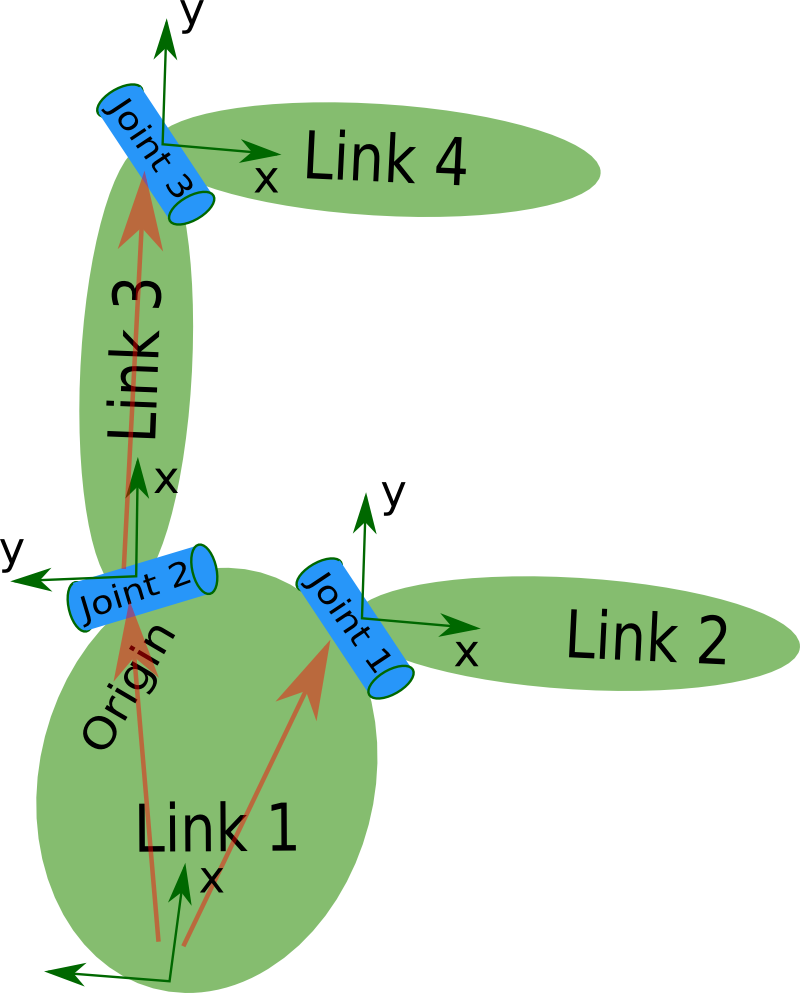
\includegraphics[height=0.3\textwidth]{img/links-joints.png}
% 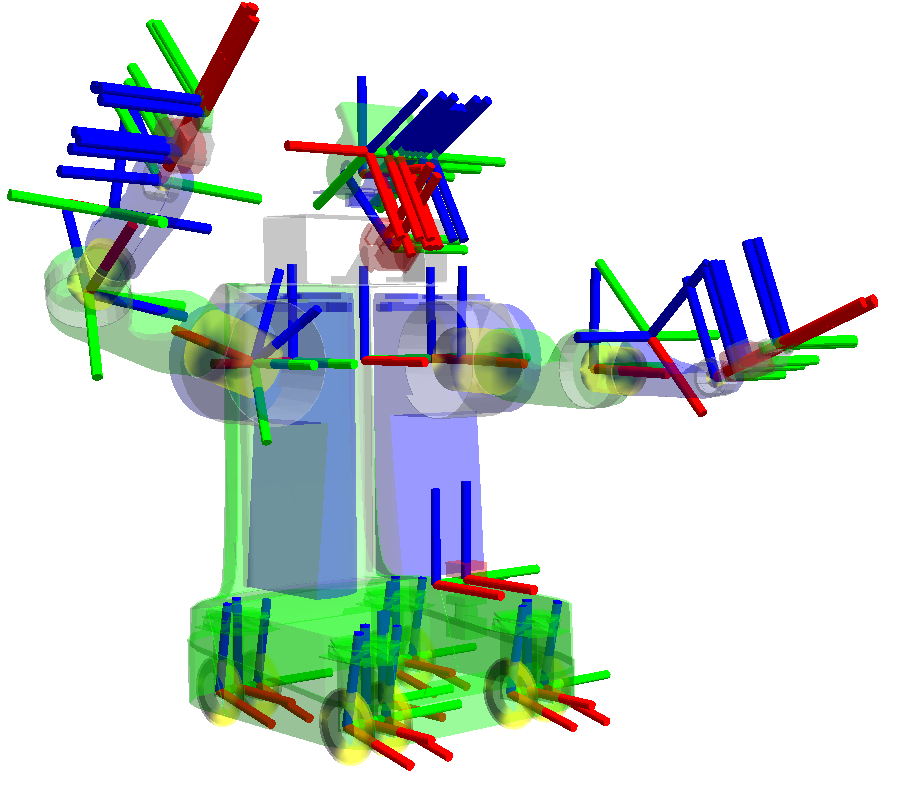
\includegraphics[height=0.3\textwidth]{img/tf-frames.png}
% \end{center}

Pose data is saved in \mongodb collections named ``tf'', the format is described below.

%%%%%%%%%%%%%%%%%%%%%%%%%%%%%%%%%
%%%%%%%%%%%%%%%%%%%%%%%%%%%%%%%%%
\subsubsection{Format}
The pose data structure has
fields for encoding the translation and rotation of a coordinate frame.
The parent frame and time stamp of pose estimation
are stored in the \emph{header} field of the data structure.
The transform coordinate frame is assigned to the \emph{child\_frame\_id} field.

The data is stored in the DB collection as array.
Each array holding pose estimates for distinct frames
at the same time stamp.
For indexed search, it is important that each array
member has the same time stamp. \\

\def\arraystretch{1.1}%
\begin{figure}[htb]
\begin{center}\begin{tabular}{ >{\ttfamily}p{3.5cm} >{\ttfamily}p{2cm} p{5cm} }
\toprule
\bf Field   & \bf Type & \bf Description \\ \midrule
tf			& [dict]	& -- \\
\ \ header		& dict		& -- \\
\ \ \ \ seq		& uint32	& consecutively increasing ID \\
\ \ \ \ stamp		& time		& time stamp of this transform \\
\ \ \ \ frame\_id	& string	& parent coordinate frame of this transform \\
\ \ child\_frame\_id	& string	& coordinate frame of this transform \\
\ \ transform		& dict		& -- \\
\ \ \ \ translation	& dict		& -- \\
\ \ \ \ \ \ x		& float64	& \emph{x} axis translation \\
\ \ \ \ \ \ y		& float64	& \emph{y} axis translation \\
\ \ \ \ \ \ z		& float64	& \emph{z} axis translation \\
\ \ \ \ rotation	& dict		& -- \\
\ \ \ \ \ \ x		& float64	& \emph{x} component of quaternion \\
\ \ \ \ \ \ y		& float64	& \emph{y} component of quaternion \\
\ \ \ \ \ \ z		& float64	& \emph{z} component of quaternion \\
\ \ \ \ \ \ w		& float64	& \emph{w} component of quaternion \\
\bottomrule
\end{tabular}\end{center}
\caption{The pose data structure in the \ease system.}
\label{fig:pose_data}
\end{figure}

Note that static frames may be recorded at lower frequency --
about every two seconds.
This usually reduces the data size significantly.
At the moment, no other motion data compression,
such as motion JPEG, is supported.

% From ``Compression of Motion Capture Databases'' Okan Arikan
% The biggest goal of compression is creating a compressed rep-
% resentation of motion that is perceptually as close to the original
% motion as possible. As we will explore later in this paper, a small
% numerical error does not necessarily correspond to a perceptually
% close motion. We would like compression and decompression to be
% as quick as possible. In practice motion capture databases can be
% very big. Therefore another goal for compression and decompres-
% sion is to be able to process without holding the entire database in
% the memory, which may not be possible. Depending on the appli-
% cation we may want to “stream” the data so that the decompressor
% can decode incrementally. We may also want to be able to decode a
% piece of the database without having to decompress any other mo-
% tion

%%%%%%%%%%%%%%%%%%%%%%%%%%%%%%%%%
%%%%%%%%%%%%%%%%%%%%%%%%%%%%%%%%%
\subsubsection{Symbol Abstraction}
%%%%%%%%%%%%%%%%%%%%%%%%%%%%%%%%%
\begin{center}
\begin{tabular}{ >{\ttfamily\bf}p{3.5cm} >{\ttfamily}p{8.2cm} }
\toprule
Module  & knowrob\_objects\footnote{\url{https://github.com/knowrob/knowrob/tree/master/knowrob\_objects}} \\
Symbols & object pose \\
Implementation & Prolog \\
\bottomrule
\end{tabular}
\end{center}
\begin{description}
\item[\textbf{belief\_at(Object, [Parent,Child,Translation,Rotation], Instant)}]
This temporal predicate computes a Prolog-based pose representation (2nd argument)
for a named object (1st argument). Time is supplied to the predicate as time stamp
(3rd argument).
\end{description}

%%%%%%%%%%%%%%%%%%%%%%%%%%%%%%%%%
\begin{center}
\begin{tabular}{ >{\ttfamily\bf}p{3.5cm} >{\ttfamily}p{8.2cm} }
\toprule
Module  & comp\_spatial\footnote{\url{https://github.com/knowrob/knowrob/tree/master/comp\_spatial}} \\
Symbols & spatial relations \\
Implementation & Prolog \\
\bottomrule
\end{tabular}
\end{center}


\begin{description}
\item[\textbf{comp\_inCenterOf(Inner,Outer,Interval)}]
Check if \owlClass{Inner} is in the center of \owlClass{Outer}.
Currently does not take the orientation into account, only the position and dimension.
Computes the \owlPredicate{inCenterOf} relation.

\item[\textbf{comp\_inFrontOf(Front,Back,Interval)}]
Check if \owlClass{Front} is in front of \owlClass{Back}.
Currently does not take the orientation
into account, only the position and dimension.
Computes the \owlPredicate{inFrontOf-Generally} relation.

\item[\textbf{comp\_inContGeneric(Inner,Outer,Interval)}]
True iff the object \owlClass{Inner} is inside 
of the bounding box of container \owlClass{Outer} during
the specified interval.
Computes the \owlPredicate{in-ContGeneric} relation.

\item[\textbf{comp\_onPhysical(Top,Bottom,Interval)}]
Check if \owlClass{Top} is in the area of and above \owlClass{Bottom}.
Computes the \owlPredicate{on-Physical} relation

\item[\textbf{comp\_above(Top,Bottom,Interval)}]
Check if \owlClass{Top} is in the area of and above \owlClass{Bottom}.
Computes the \owlPredicate{above-Generally} relation.

\item[\textbf{comp\_below(Bottom,Top,Interval)}]
Check if \owlClass{Top} is in the area of and above \owlClass{Bottom}.
Computes the \owlPredicate{below-Generally} relation.

\item[\textbf{comp\_toTheLeftOf(Left,Right,Interval)}]
Check if \owlClass{Left} is to the left of \owlClass{Right}.
Currently does not take the orientation
into account, only the position and dimension.
Computes the \owlPredicate{toTheLeftOf} relation.

\item[\textbf{comp\_toTheRightOf(Right,Left,Interval)}]
Check if \owlClass{Left} is to the left of \owlClass{Right}.
Currently does not take the orientation
into account, only the position and dimension.
Computes the \owlPredicate{toTheRightOf} relation.
\end{description}


%%%%%%%%%%%%%%%%%%%%%%%%%%%%%%%%%
%%%%%%%%%%%%%%%%%%%%%%%%%%%%%%%%%
% \section{Image Data}
% \input{content/neem-experience/image-data}

%%%%%%%%%%%%%%%%%%%%%%%%%%%%%%%%%
%%%%%%%%%%%%%%%%%%%%%%%%%%%%%%%%%
% \section{Gaze Data}
% \input{content/neem-experience/gaze-data}

%%%%%%%%%%%%%%%%%%%%%%%%%%%%%%%%%
%%%%%%%%%%%%%%%%%%%%%%%%%%%%%%%%%
% \section{EEG Data}
% \input{content/neem-experience/eeg-data}


\setcounter{section}{0}

\chapter{NEEM-Background}
\label{ch:background}
\chapterauthor{D. Be{\ss}ler, M. Pomarlan, A. Vyas}

The \neembak represents the (physical) context of \neems.
More concretely, the \neembak represents the environment where events took place, and the agents that are involved.
These are representations of physical objects, their parts, properties, and relationships between them.

Each \neem must have exactly one associated \neembak.
This is important as only the objects and their properties represented in the \neembak may be involved in events that occur in \neems.
Consider, for example, a robot fetching a cup in a kitchen environment to prepare a coffee.
The cup would be part of the \neembak while the fetching event carried out by the robot would be represented in the \neemnar (Chapter~\ref{ch:narrative}).

The way how a task can be solved best depends on what is available in the environment.
The suitability of an object to be used to perform a certain task is often derived from the class of objects it belongs to, e.g., a knife can be used for cutting.
The \neem model defines a set of more general object classes such as \emph{agent} and \emph{artifact} (Section~\ref{sec:background:types}).
These are used to classify each object represented in the \neembak.
%
The usability of an object is, however, ultimately grounded in its properties, e.g., a dulled knife may prove to be unusable to perform a cutting task.
It is thus also relevant to characterize object properties as they correlate with how an agent may solve its task.
Consequently, we treat types of object properties as classes organized in a taxonomy (Section~\ref{sec:background:properties}).

\neems may characterize different aspects of the environment depending on what information is accessible when the \neem is acquired.
We organize different characteristics in so called \emph{views} (Section~\ref{sec:background:views}).
Each view has its own set of types and relationships to represent the environment from a specific viewpoint such as appearance or kinematics.

\neems are heterogeneous representations that may include additional data files.
These representations are time series data that are annotated by the \neemnar.
In addition, some widely used data formats for the representation of objects are supported (Section~\ref{sec:background:formats}).
Such data files may be stored within the \neembak, associated to objects it represents, and used to enrich knowledge about the environment.

%%%%%%%%%%%%%%%%%%%%%%%%%%%%%%%%%%%%%%%%%%%%%%%
%%%%%%%%%%%%%%%%%%%%%%%%%%%%%%%%%%%%%%%%%%%%%%%
\section{Types of Objects}
\label{sec:background:types}

Objects and agents that appear in an environment are classified as \emph{physical objects}.
Physical objects are exactly the objects you can point to, as they have a location in space.

The most common physical objects in non-natural environments are \emph{artifacts}.
An artifact is an item that has certain structure, often to serve a particular purpose such as to use it in a certain way, or to enjoy looking at it in case of, e.g., an art piece.
Artifacts that were created with a purpose in mind are called \emph{designed artifacts}.
Most objects in human-made environments belong to this category.
Note that, e.g., a \emph{container} is not a designed artifact, as also objects that were not designed as such may serve as containers.
Consequently, the class \emph{designed container} is used for the objects that were designed to be used as a container.
Other examples of designed artifacts are \emph{tools} and \emph{appliances} designed for specific tasks or agents and the \emph{components} designed to fit together to form a larger whole.

Another category of objects are \emph{physical bodies}.
Most commonly one would use this category for \emph{substances} that appear in the environment such as a blob of dough, or the coffee inside of a cup.
However, it is more appropriate to classify the substance as \emph{designed substance} in case it was created with a purpose in mind, for e.g., in the case for the dough that is made according to a recipe and supposed to be eaten after being baked.

Agents that appear in a \neem are classified as \emph{physical agents}.
The difference from other types of objects is that the agents have intentions, execute actions, and attempt to achieve goals, e.g., by following a plan and moving their body in a way to generate interactions with the environment to cause intended effects.
Each agent is composed of \emph{functional parts} organized in a skeletal structure.
Interactions with the environment are carried out through \emph{effectors} such as arms, legs, or hands.
Effectors that are used for grasping are called \emph{prehensile effectors}.

The last top-level category in our object taxonomy is \emph{physical place}.
Places are objects with a specific location such as the surface of a table, or the campus of the University.
Each \neem refers at least to the place where it was acquired, which is usually a room in a building with objects that can be used to perform certain everyday tasks.

%According to \dul~\footnote{\url{http://www.ontologydesignpatterns.org/ont/dul/DUL.owl}} upper level ontology, an object participates in an event during its lifetime and has its own spatial location. During an everyday activity, we come across many objects which are mainly of physical type. A physical object is defined as an object that has a proper space region and associated mass. Sub-classes of physical objects are dirty object, physical agent, physical artifact, physical body, physical space, and physical effector. A typical object participate in an event and can be classified by role. It can have physical qualities such as color, localization, disposition, capacity, shape, size, and temperature that are aspect of an object dependent on its physical manifestation. 

%An object branch also covers a design taxonomy which considers functional, structural and aesthetic aspect of object design. Designs are useful to support an agent to hypothesize unknown functions that can be served by an entity\todo{Seba; What exactly is en entity ? An object ? an instance of a concept ?}. A design describes objects which host a common design relevant qualities such as, dispositional, geometrical, and aesthetic. An intelligent agent would be able to infer based on dispositional quality of an object if it can be used to serve other function in everyday task. For example, a heavy door stopper would also be able to function as paper weight or a dining table can be also used as ping pong table based on appropriate dimensions.

%%%%%%%%%%%%%%%%%%%%%%%%%%%%%%%%%%%%%%%%%%%%%%%
%%%%%%%%%%%%%%%%%%%%%%%%%%%%%%%%%%%%%%%%%%%%%%%
\section{Properties of Objects}
\label{sec:background:properties}

Qualities are the properties of an object that are not part of it, but cannot exist without it.
This is, for example, the quality of having a shape -- a quality inherited by all physical objects.
Another example is the quality of a floor having a certain surface friction and thus being slippery or not.
A robot navigating on such a floor could use this knowledge to avoid, for example,
spillage when moving on the floor with a coffee-filled cup.
The quality concept does not directly encode the value of the object property, but only focuses on characteristics of the property itself.
This is mainly useful in cases where individual aspects of an entity are considered in the domain of discourse.

\begin{ODP}{Object Qualities}
	\ODPINTENT{To represent the qualities of an object.}
	\ODPDEFINEDIN{DUL.owl}
	\ODPQUESTION{What qualities does this object have? What objects have this quality?}
	\ODPGRAPHIC{
	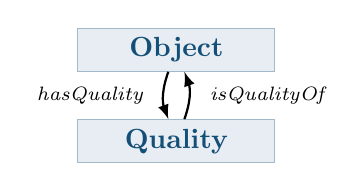
\begin{tikzpicture}
	    \node[owlclass] (A) {Object};
	    \node[owlclass,below=0.6cm of A] (B) {Quality};
	    \draw (A) edge[relationxl] node[midway,label=left:hasQuality] {} (B);
	    \draw (B) edge[relationxr] node[midway,label=right:isQualityOf] {} (A);
 %\node[owlclass] (QUALITY) {
 %\begin{owlclass}{Quality}
 % \item $(\exists \emph{isQualityOf}.\texttt{Entity})$
 % \item $(\exists \emph{hasRegion}.\texttt{Region})$
 %\end{owlclass}
 %};
 %\node[owlclass,below=0.6cm of QUALITY] (REGION) {
 %\begin{owlclass}{Region}
 % \item $(\exists \emph{isRegionFor}.\texttt{Quality})$
 %\end{owlclass}
 %};
 %\draw (QUALITY) edge[thick,-,dashed,blue!60] (REGION);
	\end{tikzpicture}
	}
	%% Example KnowRob language expressions
	\ODPEXAMPLES{
		\emph{has\_quality($o$,$q$)} &
		$q \in \abox$ is a quality of $o \in \abox$
	}
\end{ODP}

Several sub-classes of \concept{Quality} and corresponding sub-relations of \relation{has-quality} are defined in the \neem model.
Some of them will be described later in this chapter.

Each object property has one value at a time.
The value is an element in a dimensional space.
Such a dimensional space is called \concept{Region} in the \neem model.
A region may have an infinite number of elements, or, in the other case, may enumerate all its elements.
The color of an object, for example, may have a value encoded as RGB vector which is an element of the RGB colorspace (which is a region).
Regions may further be decomposed into sub-regions, for example, to represent the sub-region of RGB colorspace with dominant red color.
%The value of an object property is called \emph{Region}.
%The value itself is an element, or a sub-region in some dimensional space such as \concept{TimeInterval} or \concept{SpaceRegion}.
%A region may be a finite set of discrete labels, allowing for ``qualitative'' descriptions, but more often a region is some dimensional space allowing ``quantitative'' descriptions.
%A Region may contain a single point, in cases where the value of a property is known precisely.
Note that the domain of the relation \relation{has-region} is not \concept{Quality} but \concept{Entity}.
This is to allow assigning regions to entities without requiring an explicit \concept{Quality} individual as an intermediate. Instead, the property connecting the \concept{Entity} specifies what information the \concept{Region} conveys about the object.

As an example, a \concept{PhysicalObject} would be linked via a \relation{hasMassAttribute} to a \concept{MassAttribute}, that is, to a \concept{Region} individual containing information about the object's mass. It is the relation \relation{hasMassAttribute} that specifies what information the \concept{Region} contains.

\begin{ODP}{Regions}
	\ODPINTENT{To represent values of attributes of things.}
	\ODPDEFINEDIN{DUL.owl}
	\ODPQUESTION{What is the value for the attribute of that entity? Which entities have a certain value on that parameter/attribute/feature?}
	\ODPGRAPHIC{
	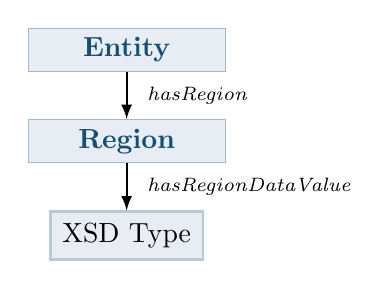
\begin{tikzpicture}
	    \node[owlclass] (A) {Entity};
	    \node[owlclass,below=0.6cm of A] (B) {Region};
	    \node[data,below=0.6cm of B] (C) {XSD Type};
	    \draw (A) edge[relation] node[midway,label=right:hasRegion] {} (B);
	    \draw (B) edge[relation] node[midway,label=right:hasRegionDataValue] {} (C);
	\end{tikzpicture}
	}
	%% Example KnowRob language expressions
	\ODPEXAMPLES{
		\emph{has\_region($x$,$y$)} &
		$y$ is a region of $x$ \\
		% % % % %
		\emph{has\_data\_value($x$,$y$)} &
		$y$ is a data value of $x$ 
	}
\end{ODP}

%%%%%%%%%%%%%%%%%%%%%%%%%%%%%%%%%%%%%%%%%%%%%%%
%%%%%%%%%%%%%%%%%%%%%%%%%%%%%%%%%%%%%%%%%%%%%%%
\section{Views on Objects}
\label{sec:background:views}

The \neembak may represent several different \emph{views} on the same object highlighting different characteristics that are fused in the \neembak to form a more complete representation of the environment.
Each view has its own vocabulary to describe objects including view-specific types of objects, qualities, and relations, and has a distinct set of competency questions that may be answered in case a \neem represents the view.
A \neem may not represent each supported view, however, it is recommended to represent as many as possible.

%%%%%%%%%%%%%%%%%%%%%%%%%%%%%%%%%%%%%%%%%%%%%%%
\subsection{Appearance}

SOMA defines several concepts to represent qualities relating to an object's appearance. The list includes, but is not limited to, 
\concept{Color}, \concept{Shape}, and \concept{Size} %, \concept{Sharpness}
.
A quality belongs to an object, and can take values only from regions of an appropriate type.

%A \emph{ShapeRegion} individual can further be classified 
The shape of an object can either be represented
as primitive geometry
(e.g., box or cylinder),
%(e.g. \emph{BoxShape}, \emph{CylinderShape}),
or as mesh. %\emph{MeshShape}.
%This finer classification decides what data is attached to the individual.
Primitive shapes are described by their geometric parameters, such as height, width and length for a box, and radius and length for a cylinder.
A mesh shape, on the other hand, has a data property that is a URI of the file that contains the mesh data.
%To fill in shape data for a shape region, it is necessary to provide data items -- floats or URIs -- and link them via the appropriate data properties to the region individual.
\todo{MP: the ontology defines hasDepth and hasHeight for BoxShape. I assume this is a mistake and we want hasLength and hasHeight. DB: I believe this is a ROS convention}
\todo{DB: where is a shape located? the origin of a shape may not be the same as the one of the object}
\todo{DB: the scale for the mesh is missing!}

\begin{ODP}{Shape Quality}
	\ODPINTENT{To represent the quality of having a shape.}
	\ODPDEFINEDIN{SOMA.owl}
	\ODPQUESTION{Does this objects have a shape?}
	\ODPGRAPHIC{
	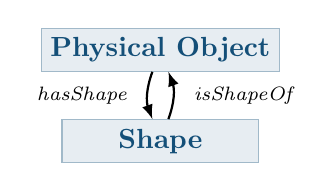
\begin{tikzpicture}
	    \node[owlclass] (A) {Physical Object};
	    \node[owlclass,below=0.6cm of A] (B) {Shape};
	    %\node[owlclass,below=0.6cm of B] (C) {Shape Region};
	    \draw (A) edge[relationxl] node[midway,label=left:hasShape] {} (B);
	    \draw (B) edge[relationxr] node[midway,label=right:isShapeOf] {} (A);
	    %\draw (B) edge[relationxl] node[midway,label=left:hasShapeRegion] {} (C);
	    %\draw (C) edge[relationxr] node[midway,label=right:isShapeRegionOf] {} (B);
	\end{tikzpicture}
	}
	%% Example KnowRob language expressions
	\ODPEXAMPLES{
		\emph{has\_shape($o$)}     & $o \in \abox$ has a shape \\
		\emph{has\_shape($o$,$s$)} & $s \in \abox$ is the shape of $o \in \abox$
	}
\end{ODP}

\begin{ODP}{Shape Region}
	\ODPINTENT{To represent the region of shapes.}
	\ODPDEFINEDIN{SOMA.owl}
	\ODPQUESTION{What geometric parameters has this shape?
		What is the URL where a mesh file of this shape can be retrieved?}
	\ODPGRAPHIC{
	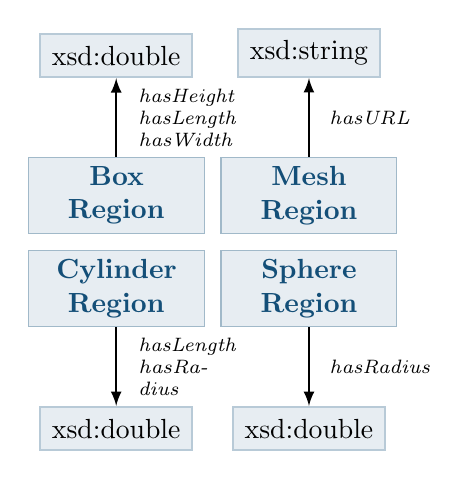
\begin{tikzpicture}
	    \node[owlclass_f] (A1) {Box Region};
	    \node[owlclass_f,right=0.2cm of A1] (A3) {Mesh Region};
	    \node[owlclass_f,below=0.2cm of A1] (A2) {Cylinder Region};
	    \node[owlclass_f,right=0.2cm of A2] (A4) {Sphere Region};
	    \node[data,above=1.0cm of A1] (B1) {xsd:double};
	    \node[data,below=1.0cm of A2] (B2) {xsd:double};
	    \node[data,above=1.0cm of A3] (B3) {xsd:string};
	    \node[data,below=1.0cm of A4] (B4) {xsd:double};
	    \draw (A4) edge[relation,xshift=0.0cm] node[midway,label=right:hasRadius] {} (B4);
	    \draw (A3) edge[relation,xshift=0.0cm] node[midway,label=right:hasURL] {} (B3);
	    \draw (A1) edge[relation,xshift=0.0cm]
	    	node[midway,text width=1.2cm,xshift=0.9cm] {hasHeight hasLength hasWidth} (B1);
	    \draw (A2) edge[relation,xshift=0.0cm]
	    	node[midway,text width=1.2cm,xshift=0.9cm] {hasLength hasRadius} (B2);
	    %\node[owlclass_f,below=0.8cm of A1] at ($(A1)!0.5!(A3)$) (C) {Shape};
	    %\draw (C) edge[relation] node[midway,label=left:hasRegion] {} (A1);
	    %\draw (C) edge[relation] node[midway,label=left:hasRegion] {} (A2);
	    %\draw (C) edge[relation] node[midway,label=right:hasRegion] {} (A3);
	    %\draw (C) edge[relation] node[midway,label=right:hasRegion] {} (A4);
	\end{tikzpicture}
	}
	%% Example KnowRob language expressions
	\ODPEXAMPLES{
		\emph{has\_bbox($o$,$d$,$w$,$h$)} &
		$d,w,h \in \mathbb{R}$ are the depth, width and height of the bounding box of $o \in \abox$ \\
		% % % % %
		\emph{has\_shape\_data($o$,sphere($r$))} &
		$r \in \mathbb{R}$ is the radius of the sphere shape of $o \in \abox$
	}
\end{ODP}

\iffalse
\begin{ODP}{Specifying a MeshShape}
	\ODPINTENT{To link to data about an arbitrary shape.}
	\ODPDEFINEDIN{SOMA.owl}
	\ODPQUESTION{What quantitative data is available about the shape of an object?}
	\ODPGRAPHIC{
	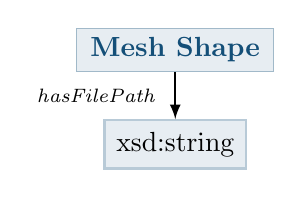
\begin{tikzpicture}
	    \node[owlclass] (A) {Mesh Shape};
	    \node[data,below=0.6cm of A] (B) {xsd:string};
	    \draw (A) edge[relation] node[midway,label=left:hasFilePath] {} (B);
	\end{tikzpicture}
	}
	%% Example KnowRob language expressions
	\ODPEXAMPLES{\emph{xxx\_xxxxx($x$,$y$)} & \textbf{todo}}
\end{ODP}
\fi

The color of an object is a quality that may take values from a \emph{ColorRegion}. Color regions may be qualitative, such as \emph{GreenColor} or \emph{RedColor}, which correspond to sets of color values; color regions may also be specified as a single datapoint, i.e. a string representing the color's components in some color space. \todo{MP: Decide how to represent color values and color spaces in the ontology, and push axioms to this effect.}
\todo{DB: most objects have many colors, how is this handled?}
\todo{DB: color does not remain constant as the light in the environment changes, how is this handled?}
\todo{DB: is material represented?}

\begin{ODP}{Color Quality}
	\ODPINTENT{To represent the quality of having a color.}
	\ODPDEFINEDIN{SOMA.owl}
	\ODPQUESTION{Does this objects have a color?}
	\ODPGRAPHIC{
	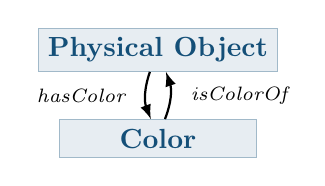
\begin{tikzpicture}
	    \node[owlclass] (A) {Physical Object};
	    \node[owlclass,below=0.6cm of A] (B) {Color};
	    \draw (A) edge[relationxl] node[midway,label=left:hasColor] {} (B);
	    \draw (B) edge[relationxr] node[midway,label=right:isColorOf] {} (A);
	\end{tikzpicture}
	}
	%% Example KnowRob language expressions
	\ODPEXAMPLES{
		\emph{has\_color($o$)}     & $o \in \abox$ has a color \\
		\emph{has\_color($o$,$c$)} & $c \in \abox$ is the color of $o \in \abox$
	}
\end{ODP}

\begin{ODP}{Color Region}
	\ODPINTENT{To represent the color of physical objects.}
	\ODPDEFINEDIN{SOMA.owl}
	\ODPQUESTION{What is the color of this object? Which objects have this color?}
	\ODPGRAPHIC{
	\begin{tikzpicture}
	    \node[owlclass,below=0.6cm of B] (C) {Color Region};
	    \node[data,below=0.6cm of C] (D) {xsd:string};
	    \draw (C) edge[relation] node[midway,label=right:hasRGBValue] {} (D);
	\end{tikzpicture}
	}
	%% Example KnowRob language expressions
	\ODPEXAMPLES{
		\emph{object\_color\_rgb($o$,$[r,g,b]$)} &
		$r,g,b \in \mathbb{R}$ is the RGB color data of $o \in \abox$
	}
\end{ODP}

%%%%%%%%%%%%%%%%%%%%%%%%%%%%%%%%%%%%%%%%%%%%%%%
\subsection{Structure}

Parthood represents that objects are composed of smaller things.
These things may be physical objects themselves, and a \emph{component} of their direct parent in the partonomy.
Parthood is transitive, that is, parts of parts are parts again, but componency is not.
So one would say that the arm is a component of the robot, and that the elbow is component of the arm, but not that the elbow is a component of the robot -- however the elbow is a part of the robot due to the transitivity of the parthood relation.

\begin{ODP}{Components}
	\ODPINTENT{To represent proper parthood of objects.}
	\ODPDEFINEDIN{DUL.owl}
	\ODPQUESTION{What is this object component of? What are the components of this object?}
	\ODPGRAPHIC{
	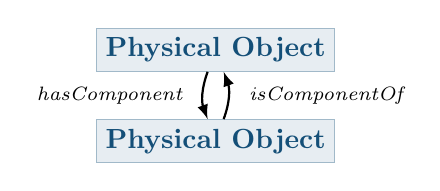
\begin{tikzpicture}
	    \node[owlclass] (A) {Physical Object};
	    \node[owlclass,below=0.6cm of A] (B) {Physical Object};
	    \draw (A) edge[relationxl] node[midway,label=left:hasComponent] {} (B);
	    \draw (B) edge[relationxr] node[midway,label=right:isComponentOf] {} (A);
	\end{tikzpicture}
	}
	%% Example KnowRob language expressions
	\ODPEXAMPLES{
		\emph{has\_component($x$,$y$)} &
		$y \in \abox$ is a component of $x \in \abox$
	}
\end{ODP}

However, another parthood type is needed for objects such as holes, bumps, boundaries, or spots of color that are physical parts but not a proper component of their parent in the partonomy.
These are \emph{features} of the object.
Features are usually localized in the object reference frame, and may carry additional properties describing, for example, the size of the hole, or the color of the spot.

\begin{ODP}{Features}
	\ODPINTENT{To represent features of objects.}
	\ODPDEFINEDIN{SOMA.owl}
	\ODPQUESTION{What are the features of this object? What are the objects with this feature?}
	\ODPGRAPHIC{
	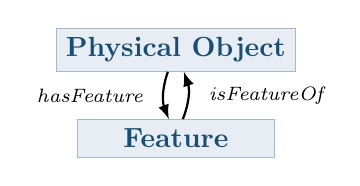
\begin{tikzpicture}
	    \node[owlclass] (A) {Physical Object};
	    \node[owlclass,below=0.6cm of A] (B) {Feature};
	    \draw (A) edge[relationxl] node[midway,label=left:hasFeature] {} (B);
	    \draw (B) edge[relationxr] node[midway,label=right:isFeatureOf] {} (A);
	\end{tikzpicture}
	}
	%% Example KnowRob language expressions
	\ODPEXAMPLES{
		\emph{has\_feature($x$,$y$)} &
		$y \in \abox$ is a feature of $x \in \abox$
	}
\end{ODP}

%%%%%%%%%%%%%%%%%%%%%%%%%%%%%%%%%%%%%%%%%%%%%%%
\subsection{Kinematics}

Kinematics, also often referred to as \emph{geometry of motion}, describes how objects may move without considering the influence of forces.
The kinematic state of an object is given by its pose over time, stored in the \neemexp as time-series data, and accessed via a dedicated predicate \emph{is\_at}.
Poses are expressed within a frame of reference.
There is one reference frame at the origin of each object, and possibly more at the various locations of interest.
In addition, there is one dedicated root reference frame, the origin of the map.
Each other frame must be, possibly indirect, connected to the map origin frame.
The pose itself is given as 6D pose including the objects' orientation as quaternion vector.

\begin{ODP}{Localization}
	\ODPINTENT{To represent that objects are localized in a map.}
	\ODPDEFINEDIN{SOMA.owl}
	\ODPQUESTION{Is this object localized?
			In which map is this object localized?
			What are the objects localized in this map?}
	\ODPGRAPHIC{
	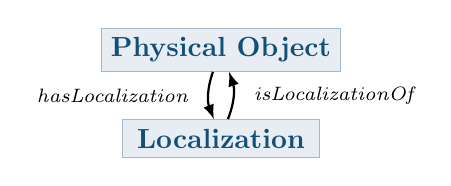
\begin{tikzpicture}
	    \node[owlclass] (A) {Physical Object};
	    \node[owlclass,below=0.6cm of A] (B) {Localization};
	    %\node[owlclass,below=0.6cm of B] (C) {Physical Place};
	    \draw (A) edge[relationxl] node[midway,label=left:hasLocalization] {} (B);
	    \draw (B) edge[relationxr] node[midway,label=right:isLocalizationOf] {} (A);
	    %\draw (B) edge[relationxl] node[midway,label=left:hasOrigin] {} (C);
	    %\draw (C) edge[relationxr] node[midway,label=right:isOriginOf] {} (B);
	\end{tikzpicture}
	}
	%% Example KnowRob language expressions
	\ODPEXAMPLES{
		\emph{is\_localized($o$)} &
		$o \in \abox$ is localized wrt. some map origin \\
		\emph{is\_localized($o$,$m$)} &
		$o \in \abox$ is localized wrt. the origin of $m \in \abox$
	}
\end{ODP}

\begin{ODP}{Pose Data}
	\ODPINTENT{To represent kinematic trees of objects connected via joints.}
	\ODPDEFINEDIN{SOMA.owl}
	\ODPQUESTION{Are these objects kinematically coupled?
			Which objects are linked through this joint?}
	\ODPGRAPHIC{
	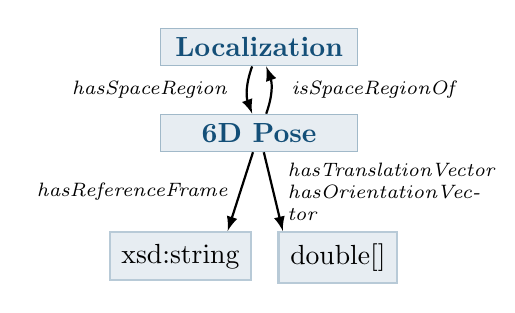
\begin{tikzpicture}
	    \node[owlclass] (A) {Localization};
	    \node[owlclass,below=0.6cm of A] (B) {6D Pose};
	    \node[data,below=1.0cm of B,xshift=1.0cm] (C) {double[]};
	    \node[data,below=1.0cm of B,xshift=-1.0cm] (D) {xsd:string};
	    \draw (A) edge[relationxl] node[midway,label=left:hasSpaceRegion] {} (B);
	    \draw (B) edge[relationxr] node[midway,label=right:isSpaceRegionOf] {} (A);
	    \draw (B) edge[relation,xshift=-0.4cm] node[midway,xshift=0.1cm,label=left:hasReferenceFrame]
	      {} ($(D.north-|B)$);
	    \draw (B) edge[relation,xshift=0.3cm] node[midway,text width=2.4cm,xshift=1.4cm]
	    	{hasTranslationVector hasOrientationVector} ($(C.north-|B)$);
	\end{tikzpicture}
	}
	%% Example KnowRob language expressions
	\ODPEXAMPLES{
		\emph{is\_at($o$,[$x$,$\vec{p}$,$\vec{q}$]) \emph{during} $\vec{ti}$} &
		$\vec{p} \in \mathbb{R}^3$ is the position, and $\vec{q} \in \mathbb{R}^4$ the orientation of $o \in \abox$ within the reference frame $x \in \mathcal{F}$ during time interval $\vec{ti} \in \mathbb{R}^2_{\geq 0}$
	}
\end{ODP}

However, objects often can not move freely but are constrained in their movement with respect to some reference object.
This is, for example, the case for walls without doors preventing movement from one room to another, or for two objects that are attached to each other via a \emph{joint} and thus restricting movement relative to each other (kinematic coupling).
Kinematically coupled objects are often part of a bigger hierarchical structure, and one of the linked objects, the parent link of the joint, is the one closer to the root of the structure then followed by the child link of the joint.

\begin{ODP}{Joints}
	\ODPINTENT{To represent kinematic trees of objects connected via joints.}
	\ODPDEFINEDIN{SOMA.owl}
	\ODPQUESTION{Are these objects kinematically coupled?
			Which objects are linked through this joint?}
	\ODPGRAPHIC{
	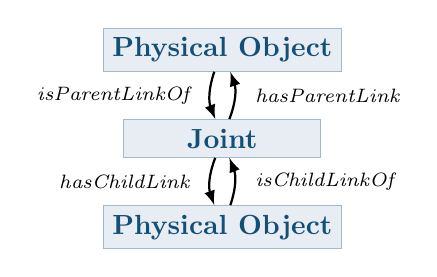
\begin{tikzpicture}
	    \node[owlclass] (A) {Physical Object};
	    \node[owlclass,below=0.6cm of A] (B) {Joint};
	    \node[owlclass,below=0.6cm of B] (C) {Physical Object};
	    \draw (A) edge[relationxl] node[midway,label=left:isParentLinkOf] {} (B);
	    \draw (B) edge[relationxr] node[midway,label=right:hasParentLink] {} (A);
	    \draw (B) edge[relationxl] node[midway,label=left:hasChildLink] {} (C);
	    \draw (C) edge[relationxr] node[midway,label=right:isChildLinkOf] {} (B);
	\end{tikzpicture}
	}
	%% Example KnowRob language expressions
	\ODPEXAMPLES{
		\emph{has\_child\_link($j$,$o$)} &
		$o \in \abox$ is the child link of joint $j \in \abox$ \\
		\emph{has\_parent\_link($j$,$o$)} &
		$o \in \abox$ is the parent link of joint $j \in \abox$
	}
\end{ODP}

The pattern above is used to represent kinematical structures, however these representations must also be linked to the various typed objects that are represented in the \neembak.
Such objects may be referred to directly in kinematical structures in case of not being composed of movable parts.
In the case of having movable parts, the object corresponds to chains of links connected via joints in the kinematics representation.
This is, for example, that the kinematical chain from shoulder to wrist forms an arm component.
Each kinematic object component has exactly one root link, and may have many end links such as a hand component having its root in the wrist, and ending at each fingertip.

\begin{ODP}{Component Chains}
	\ODPINTENT{To represent the kinematic chain of object components.}
	\ODPDEFINEDIN{SOMA.owl}
	\ODPQUESTION{What is the kinematic root of this object?
			What are the end links of this object?
	}
	\ODPGRAPHIC{
	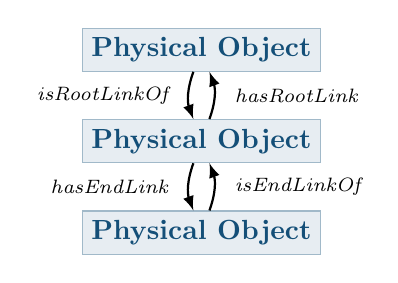
\begin{tikzpicture}
	    \node[owlclass] (A) {Physical Object};
	    \node[owlclass,below=0.6cm of A] (B) {Physical Object};
	    \node[owlclass,below=0.6cm of B] (C) {Physical Object};
	    \draw (A) edge[relationxl] node[midway,label=left:isRootLinkOf] {} (B);
	    \draw (B) edge[relationxr] node[midway,label=right:hasRootLink] {} (A);
	    \draw (B) edge[relationxl] node[midway,label=left:hasEndLink] {} (C);
	    \draw (C) edge[relationxr] node[midway,label=right:isEndLinkOf] {} (B);
	\end{tikzpicture}
	}
	%% Example KnowRob language expressions
	\ODPEXAMPLES{
		\emph{has\_base\_link($o_1$,$o_2$)} &
		$o_2 \in \abox$ is the first link of $o_1 \in \abox$ \\
		\emph{has\_end\_link($o_1$,$o_2$)} &
		$o_2 \in \abox$ is one of the last links of $o_1 \in \abox$
	}
\end{ODP}

The position of a joint determines the position of the child link relative to the parent.
Depending on whether the joint is either \emph{hinged} (rotation around an axis) or prismatic (sliding along an axis), the position is measured in radians or meter respectively.
When the position changes over time, velocity (measured in $rad/s$ or $m/s$) and effort applied in the joint (measured in $Nm$ or $N$) can be measured.
Joint states are recorded as time-series data and stored in the \neemexp.
However, the \neem model defines a set of data properties used to access joint state data.

\begin{ODP}{Joint States}
	\ODPINTENT{To represent the position of a joint.}
	\ODPDEFINEDIN{SOMA.owl}
	\ODPQUESTION{What is the state of this joint?
		What is its position and velocity?
		How much effort is applied?
	}
	\ODPGRAPHIC{
	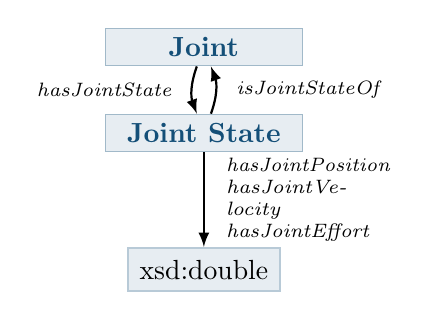
\begin{tikzpicture}
	    \node[owlclass] (A) {Joint};
	    \node[owlclass,below=0.6cm of A] (B) {Joint State};
	    \node[data,below=1.2cm of B] (C) {xsd:double};
	    \draw (A) edge[relationxl] node[midway,label=left:hasJointState] {} (B);
	    \draw (B) edge[relationxr] node[midway,label=right:isJointStateOf] {} (A);
	    \draw (B) edge[relation] node[midway,text width=2.0cm,xshift=1.3cm]
	    	{hasJointPosition hasJointVelocity hasJointEffort} (C);
	\end{tikzpicture}
	}
	%% Example KnowRob language expressions
	\ODPEXAMPLES{
		\emph{has\_joint\_position($j$,$x$)} &
		$x \in \mathbb{R}$ is the position of joint $j \in \abox$ given in $m$ (prismatic joints) or $rad$ (hinged joints) \\
		\emph{has\_joint\_velocity($j$,$v$)} &
		$v \in \mathbb{R}$ is the velocity of joint $j \in \abox$ given in $\frac{m}{s}$ (prismatic joints) or $\frac{rad}{s}$ (hinged joints) \\
		\emph{has\_joint\_effort($j$,$x$)} &
		$x \in \mathbb{R}$ is the applied force of a prismatic, or the torque of a hinged joint $j \in \abox$ given in $N$ or $N \cdot m$ respectively.
	}
\end{ODP}

The movement of a joint may be restricted by physical limits.
This is the case for \emph{revolute} and \emph{prismatic} joints.
The joint position is bounded between a minimum and maximum value, expressed as radians for revolute joints, and meters for prismatic joints.
In addition, maximum values for the velocity and effort of a joint may be provided.

\begin{ODP}{Joint limits}
	\ODPINTENT{To represent the hard limits of a joint.}
	\ODPDEFINEDIN{SOMA.owl}
	\ODPQUESTION{How far can this joint move into some direction?}
	\ODPGRAPHIC{
	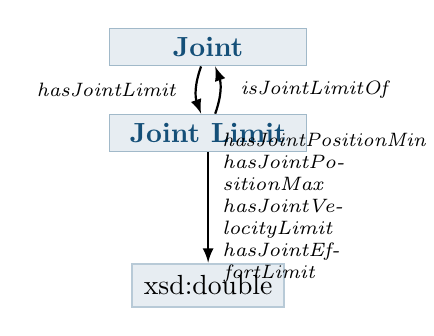
\begin{tikzpicture}
	    \node[owlclass] (A) {Joint};
	    \node[owlclass,below=0.6cm of A] (B) {Joint Limit};
	    \node[data,below=1.4cm of B] (C) {xsd:double};
	    \draw (A) edge[relationxl] node[midway,label=left:hasJointLimit] {} (B);
	    \draw (B) edge[relationxr] node[midway,label=right:isJointLimitOf] {} (A);
	    \draw (B) edge[relation] node[midway,text width=2.2cm,xshift=1.3cm]
	    	{hasJointPositionMin hasJointPositionMax hasJointVelocityLimit hasJointEffortLimit} (C);
	\end{tikzpicture}
	}
	%% Example KnowRob language expressions
	\ODPEXAMPLES{
		\emph{has\_joint\_position\_limit($j$,$\vec{x}$)} &
		$\vec{x} \in \mathbb{R}^2$ is the minimum and maximum position of joint $j \in \abox$ given in $m$ (prismatic joints) or $rad$ (hinged joints) \\
		\emph{has\_joint\_velocity\_limit($j$,$v_{max}$)} &
		$v_{max} \in \mathbb{R}$ is the maximum velocity of joint $j \in \abox$ given in $\frac{m}{s}$ (prismatic joints) or $\frac{rad}{s}$ (hinged joints) \\
		\emph{has\_joint\_effort\_limit($j$,$x_{max}$)} &
		$x_{max} \in \mathbb{R}$ is the maximum force of a prismatic, or the maximum torque of a hinged joint $j \in \abox$ given in $N$ or $N \cdot m$ respectively.
	}
\end{ODP}

%%%%%%%%%%%%%%%%%%%%%%%%%%%%%%%%%%%%%%%%%%%%%%%
\subsection{Dynamics}

The dynamics view in the \neembak is used to characterize how objects move under the influence of force.
The \neem model only considers solid objects with constant mass and dynamics governed by Newton's laws.

\begin{ODP}{Mass}
	\ODPINTENT{To represent the quantity of matter which a body contains.}
	\ODPDEFINEDIN{SOMA.owl}
	\ODPQUESTION{What is the mass of this object?}
	\ODPGRAPHIC{
	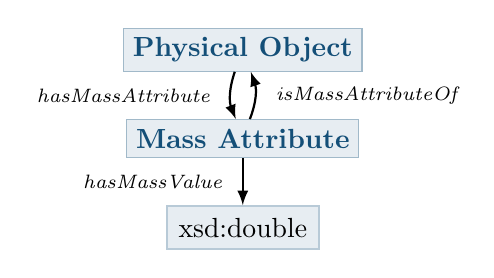
\begin{tikzpicture}
	    \node[owlclass] (A) {Physical Object};
	    \node[owlclass,below=0.6cm of A] (B) {Mass Attribute};
	    \node[data,below=0.6cm of B] (C) {xsd:double};
	    \draw (A) edge[relationxl] node[midway,label=left:hasMassAttribute] {} (B);
	    \draw (B) edge[relationxr] node[midway,label=right:isMassAttributeOf] {} (A);
	    \draw (B) edge[relation] node[midway,label=left:hasMassValue] {} (C);
	\end{tikzpicture}
	}
	%% Example KnowRob language expressions
	\ODPEXAMPLES{
		\emph{has\_mass($o$,$v$)} &
		$v \in \mathbb{R}_{>0}$ is the mass of $o \in \abox$ in kilograms
	}
\end{ODP}

At each point in time, the sum of forces influencing an object determines how its movement will change.
The accumulated force may be stored as time-series data in the \neembak, and accessed via an attribute defined in the \neem model.

\begin{ODP}{Force}
	\ODPINTENT{To represent the quantity of force influencing a solid object.}
	\ODPDEFINEDIN{SOMA.owl}
	\ODPQUESTION{What is the force acting upon this object?}
	\ODPGRAPHIC{
	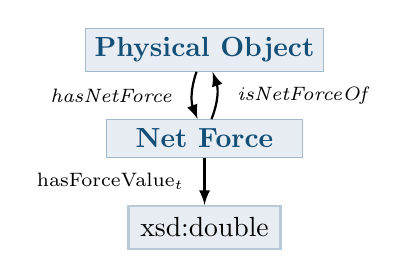
\begin{tikzpicture}
	    \node[owlclass] (A) {Physical Object};
	    \node[owlclass,below=0.6cm of A] (B) {Net Force};
	    \node[data,below=0.6cm of B] (C) {xsd:double};
	    \draw (A) edge[relationxl] node[midway,label=left:hasNetForce] {} (B);
	    \draw (B) edge[relationxr] node[midway,label=right:isNetForceOf] {} (A);
	    \draw (B) edge[relation] node[midway,label=left:$\emph{hasForceValue}_t$] {} (C);
	\end{tikzpicture}
	}
	%% Example KnowRob language expressions
	\ODPEXAMPLES{
		\emph{has\_net\_force($o$,$\vec{\f}$)} \emph{during} $\vec{ti}$ &
		$\vec{\f} \in \mathbb{R}^3$ is the accumulated force, measured in Newton, that acts upon $o \in \abox$ during time interval $\vec{ti} \in \mathbb{R}^2_{\geq 0}$
	}
\end{ODP}

\iffalse
Joints have additional physical attributes that influence how effort is translated into motion.
This is particularly relevant in case the joint is simulated.
Internal static friction force caused by movable elements within the joint, and \dots

\begin{ODP}{Joint Dynamics}
	\ODPINTENT{To represent physical attributes of joints.}
	\ODPDEFINEDIN{SOMA.owl}
	\ODPQUESTION{What are the physical attributes of this joint?}
	\ODPGRAPHIC{
	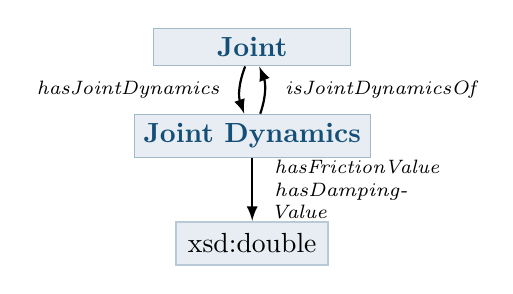
\begin{tikzpicture}
	    \node[owlclass] (A) {Joint};
	    \node[owlclass,below=0.6cm of A] (B) {Joint Dynamics};
	    \node[data,below=0.8cm of B] (C) {xsd:double};
	    \draw (A) edge[relationxl] node[midway,label=left:hasJointDynamics] {} (B);
	    \draw (B) edge[relationxr] node[midway,label=right:isJointDynamicsOf] {} (A);
	    \draw (B) edge[relation] node[midway,text width=2.0cm,xshift=1.3cm]
	    	{hasFrictionValue hasDampingValue} (C);
	\end{tikzpicture}
	}
	%% Example KnowRob language expressions
	\ODPEXAMPLES{
		\emph{has\_friction($x$,$y$)} &
		$y$ is the friction of $x$ measured in $N$ (prismatic joints) or $Nm$ (revolving joints)
	}
\end{ODP}
\fi

%%%%%%%%%%%%%%%%%%%%%%%%%%%%%%%%%%%%%%%%%%%%%%%
\subsection{Naive physics}

This view on objects is comprised of qualitative descriptions of the interactions of these objects, with a focus on how the objects could be arranged so as to constrain each other's behavior. The prototypical examples of such interactions are support and containment, but many other interactions are possible. Note, formalizing actual manifestations of such interactions as they occur in an episode will be done in chapter~\ref{ch:narrative}. In this chapter, we focus instead on ontological modelling about what kinds of interactions an object could take part in. \todo{DB: could you make explicit why this is part of the neem background? should the ease researchers manually assert dispositions of objects, or only use the ones derived from the object types?}

This is achieved by the concept of \emph{Disposition}, which is a quality that, by virtue of being possessed by an object, enables that object to participate in certain roles in certain relations or events. E.g., \emph{Deposition} and \emph{Containment} are the dispositions necessary to enable an object to act as a support or container for another.

\begin{ODP}{Friction}
	\ODPINTENT{To represent what kinds of interactions an object can participate in.}
	\ODPDEFINEDIN{SOMA.owl}
	\ODPQUESTION{What can this object be used for? Can this object interact with others in a particular way?}
	\ODPGRAPHIC{
	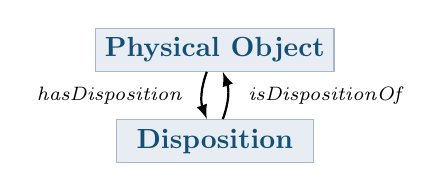
\begin{tikzpicture}
	    \node[owlclass] (A) {Physical Object};
	    \node[owlclass,below=0.6cm of A] (B) {Disposition};
	    \draw (A) edge[relationxl] node[midway,label=left:hasDisposition] {} (B);
	    \draw (B) edge[relationxr] node[midway,label=right:isDispositionOf] {} (A);
	\end{tikzpicture}
	}
	%% Example KnowRob language expressions
	\ODPEXAMPLES{
		\emph{has\_disposition($x$,$y$)} &
		$y \in \abox$ is a disposition of $x \in \abox$
	}
\end{ODP}

By and large, researchers making use of the SOMA ontology to create NEEM backgrounds and NEEMs can rely on the ontology to already provide a rich store of object knowledge, including dispositions. As such, it should usually be sufficient for the researchers adding knowledge about a new type of object, to specify the object classes defined in SOMA, to which the new object type is a subclass of. However, in case new dispositions need to be added for a new object type in the NEEM background, the above pattern illustrates how.

%%%%%%%%%%%%%%%%%%%%%%%%%%%%%%%%%%%%%%%%%%%%%%%
%%%%%%%%%%%%%%%%%%%%%%%%%%%%%%%%%%%%%%%%%%%%%%%
\section{Data Formats}
\label{sec:background:formats}

Representations in the \neembak may be enriched through additional data files.
Data files are stored with the \neembak and loaded by the \ease knowledge base when a \neem is activated.
They may encode information that can be directly represented in the \neem, however, it is not necessary in such a case to duplicate the information.
A data file may be loaded at runtime, and used by the knowledge base in combination with other representations to answer questions about an activity.

%%%%%%%%%%%%%%%%%%%%%%%%%%%%%%%%%%%%%%%%%%%%%%%
\subsection{URDF}
\label{sec:background:urdf}

The Unified Robot Description Format (URDF) is widely used for the representation of kinematics in robotics. That is how objects are organized in a skeletal structure of links and joints, and how links may move relative to each other in case of being connected via a flexible joint.
URDF was designed to represent robot kinematics.
It is, however, also often used for other types of objects with movable parts, for example to represent how a door is attached to a shelve via a joint, and what limits the joint has, but can also be used to represent completely static environments (via fixed joints).
URDF further allows to represent a set of properties for links and joints, such as what the mass of a link is, or what the hard and soft limits of a joint are.

URDF organizes objects and their parts in a common coordinate system, and represents an initial configuration of all links and joints.
The origin of this coordinate system is often called \emph{world} or \emph{map} frame.
Each object has an associated frame in this coordinate system with a position relative to the parent frame in the skeletal structure.
Frame names are further used to identify entities in the knowledge base, and logged position data that corresponds to objects described in the URDF file.

From the point of view of URDF, the world is only made of links and joints.
Joints are further classified based on how they operate, and have different sets of parameters quantifying their kinematics depending on their type.
It is, however, not possible to represent that links belong to a certain category, or that a chain of links forms a component of some type.
However, we can use the information encoded in URDF files to enrich \neembak representations, and on the other hand, use the \neembak to provide classifications for links in URDF files.

Links in URDF files may have multiple associated shapes.
Two different shape types are distinguished: collision and visualization shapes.
Each link has usually one shape of each kind.
Shapes are either represented as geometrical primitives such as spheres or boxes, or refer to an external mesh file in which case this mesh file needs to be stored as an additional data source in the \neembak (next Section).

%%%%%%%%%%%%%%%%%%%%%%%%%%%%%%%%%%%%%%%%%%%%%%%
\subsection{DAE}
\label{sec:background:dae}

The preferred format for meshes is Collada (DAE).
The reason primarily being that it is widely supported by modeling tools and rendering engines.
If possible, the mesh should be accompanied by high-resolution textures in PNG or JPG format.
The more detailed a mesh, the more immersive the experience of humans interacting with it in VR and better the perception models that can be trained by images generated by placing the object in a virtual scene. Of course, this must be balanced with the computational demands imposed by mesh rendering and collision checking. When storing mesh and texture data for objects, researchers who produce NEEM background should make sure the meshes match the demands and resources of their applications.



\setcounter{section}{0}

%%%%%%%%%%%%%%%%%%%%%%%%%%%%%%%%%%%%%%%%%%%%%%%
%%%%%%%%%%%%%%%%%%%%%%%%%%%%%%%%%%%%%%%%%%%%%%%
\section{NEEM-Narrative}
\label{ch:narrative}

The narrative part of NEEMs can be seen as a story of what has happened in terms of events that occurred, goals that were followed, and objects that were involved.
The \neemnar representation contains two basic elements: classified entities such as events and objects, and relationships between them.
The events being particularly important as their time interval is used for time-indexed data access.
Data represented in the \neemexp may further be correlated to the classes and structures in the \neemnar in order to train models that can predict the \neemnar given the \neemexp and possibly some contextual parameter.

The \neemnar model is formally defined in form of an \owl ontology which is based on the DOLCE+DnS Ultralite (DUL) upper-level ontology~\cite{DOLCE2003}.
DUL is a carefully designed ontology that seeks to model general categories underlying human cognition without making any discipline-specific assumptions.
Our extensions of DUL mainly focus on characterizing different aspects of activities that were not considered in much detail in DUL.
These extensions are part of an ontology that we have called
\soma~\footnote{\url{https://ease-crc.github.io/soma}}.
A \neemnar is made of several patterns defined either in \dul or in \soma.

While it is possible to create the representations listed in this chapter through a custom exporter, it is not advised to do so.
Instead, it is advised to interface with the
\knowrob knowledge base~\footnote{\url{https://github.com/knowrob/knowrob}}.
\knowrob provides an interface based on predicate logics that allows to interact with \neems.
The language is a collection of predicates that can be called by users to ask certain types of competency questions covering different aspects of activitiy, or to add labels and relationships in the \neemnar.
We will provide example expressions in this section that highlight how the knowledge base can be used to interact with \neems.

% % % % % % % % % % % % % % % % %
% % % % % % % % % % % % % % % % %
\subsection{Taxonomic classification}
\label{sec:taxonomy} 

\todo{Seba: Somehow here or before this seciton is some introduction text missing. It just starts randomly with a taxonomy section and jumps right away to Actions. This Action section does not mention any action taxonmoy but rather a task taxonomy}

Here in the following section, we will discuss taxonomy for the concepts used to describe \neemnar \todo{Seba: Try to use the defined latex commands to write the definitions like neem-narrative } part. A taxonomy provides the hierarchical relationships among various concepts and defines the terminology for each concept. One way to classify an entity in ontology is through taxonomies, which concentrates on \emph{what there actually is?} as compared to conceptual classification which is more about \emph{how an entity is interpreted?}. For instance, the concepts \textit{spoon} and \textit{knife} are subclasses of the concept \textit{cutlery}.

%\paragraph{Actions} 

%An action can be defined as an event where at least one agent participates, such that this agent performs a dedicated task, defined by a plan or workflow, which it executes through the Action. Here workflow refers to a plan that defines role(s), task(s), and specific structure of tasks that needs to be executed.
  
\paragraph{Task}
Task is an EventType \todo{Seba: Where is the definition of event? How many event types do exists ? Is there an event taxonmoy ? If yes, maybe we should also have an event paragraph} that classifies an Action to be executed, where an event type describes how an event should be interpreted, executed, expected, seen, etc\todo{Seba: I would avoid "etc" in definitions, especially in such general concepts. Its gives the possibitliy of interpretation and it might create an false understanding of the term, in this case event. You give an loose definition of event, however, in the previous comment I address some additional questions regarding the definition of event}\footnote{\url{http://www.ontologydesignpatterns.org/ont/dul/DUL.owl}}. For example cleaning a table is a task that can be executed by performing certain actions. However, sometimes it is hard to classify an event based on taxonomy, for such cases conceptual classification \ref{sec:classification} can explain how the task taxonomy used to classify actions.\todo{Seba: Can you elaborate this point more specific ? At this moment I am asking myself, is a sequence of actions defined as ONE task or is one action mapped to one task. Also, do I have two methods for task classification ? One method is to use taxonmical representations of actiosn to know which task they are describing. The second one is to use for the reader unknown "conceptual classification", for "difficult" classifications. What is a difficult classification ? When am I using method 1 and then method 2? } 

\todo{Seba: Where is the real difference between Task and Action ? Can I say also the action grasping executes a task grasping ? Do I only represent high level "actions" such as setting up a table as tasks ? If yes, where is the end of the abstraction ? At the motion level ?,
Answer: Agree, sometimes it is not easy to distinguish between those two. However, this is why instead of classifying them with taxonomically, we would prefer to use conceptual classification here.} 

A task can be further classified into three main categories, physical task, mental task and communication task. A task which requires to execute an action through which an agent has to manipulate representations stored in its own cognition can be categorized as mental task. Dreaming, imagining, prospecting, reasoning, retrospecting falls under mental task. Where as physical task requires an agent to perform certain physical activities such as actuating, constructing, modifying physical object, looking at, placing, navigating and perceiving. At last, communication task in which two more agents shares information. This is used to classify special kind of events that have participants as agents and social objects\todo{Seba: Is there a definition for social objects? Are social objects = agents ?}. The means of information exchange is physical however the scope of interest here is to  identify which agent communicates and what kind of information it has.
In the appendix section, we further describe all three tasks into subcategories. 

\paragraph{Motions} 
An event type which deals with movements of an agent and motions it makes during task execution.\todo{Seba: In the introduction there is mentioned there are only 2 basic elements: classified entities (events and objects) and the relationships. A simple question I have to ask, are tasks also event types? Answer: yes. Maybe a real definition of event types would be really useful. Answer: it is now provided in with task definition.} Motion taxonomy includes concepts such as 'body movement' which concentrates on the movements of agents body parts. 'Directed motion' which involves a destination and directed path for an agent to follow, however, an 'un-directed motion' is opposite to directed where agent does not have any particular destination but it is important to know that the agent has moved and motion has occurred. And at last 'fluid flow' is the process by which fluid moves or has moved from one location to other. All four concepts are further sub-categorized in appendix section.

\paragraph{Objects}
According to \dul~\footnote{\url{http://www.ontologydesignpatterns.org/ont/dul/DUL.owl}} upper level ontology, an object participates in an event during its lifetime and has its own spatial location.  describes objects into several subcategories which includes agent, digital object, feature, physical object, social object and transient \todo{Seba: Is something missing here ?}.
An object branch also covers a design taxonomy which considers functional, structural and aesthetic aspect of object design. Designs are useful to support an agent to hypothesize unknown functions that can be served by an entity\todo{Seba; What exactly is en entity ? An object ? an instance of a concept ?}. A design describes objects which host a common design relevant qualities such as, dispositional, geometrical, and aesthetic. An intelligent agent would be able to infer based on dispositional quality of an object if it can be used to serve other function in everyday task. For example, a heavy door stopper would also be able to function as paper weight or a dining table can be also used as ping pong table based on appropriate dimensions.
\todo{Seba: Will the qualities be somewhere defined ?}

\paragraph{Roles}
A social concept which is basically used for an object classification. An object can have different roles when it participates in the event during its lifetime. Role taxonomy includes agent role, answer, causal process role, communication topic, existing object role, explanation, instrument, linguistic function, location, locatum role, path role, patient, question, relatum role, and software type. Further role sub-categories will be defined under appendix section.\todo{Seba: An example with using those terms would be nice.}


% % % % % % % % % % % % % % % % %
% % % % % % % % % % % % % % % % %
\subsection{Relationships}
\subsubsection{Occurrences}
\label{sec:occurrences}
%% Summary of Figure below
The basic building blocks of \neems are the events that occur when an agent interacts with its environment through movements of its body.
An event is defined as \emph{any physical, social, or mental process, event, or state}. Events have an associated time interval that determines the time at which the event occurs. Time data is represented as unix timestamps using XSD types.
%As discussed in porevious section, we distinguish between three different event classes: \owlClass{Action}, \owlClass{State}, and \owlClass{Process}.

\begin{ODP}{Occurences1}
	\ODPINTENT{To represent the temporal extension of events.}
	\ODPDEFINEDIN{DUL.owl}
	\ODPQUESTION{What is the time interval associated to this event?}
	\ODPGRAPHIC{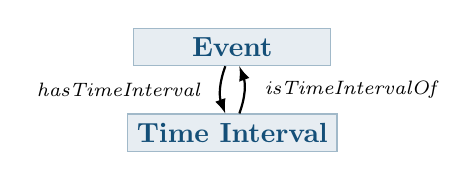
\begin{tikzpicture}
	    \node[owlclass] (A) {Event};
	    \node[owlclass,below=0.6cm of A] (B) {Time Interval};
	    \draw (A) edge[relationxl] node[midway,label=left:hasTimeInterval] {} (B);
	    \draw (B) edge[relationxr] node[midway,label=right:isTimeIntervalOf] {} (A);
	\end{tikzpicture}}
	%% Example KnowRob language expressions
	\ODPEXAMPLES{
		\emph{occurs($x$)} &
		$x$ is an occurence \\
		% % % % %
		\emph{is\_time\_interval($x$)} &
		$x$ is a time interval \\
		% % % % %
		\emph{has\_time\_interval($y$,$x$)} &
		$x$ is the time interval of event $y$
	}
\end{ODP}

\begin{ODP}{Occurences2}
	\ODPINTENT{To quantify when something has happened.}
	\ODPDEFINEDIN{SOMA.owl}
	\ODPQUESTION{When did it happen?}
	\ODPGRAPHIC{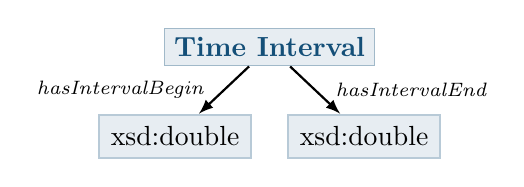
\begin{tikzpicture}
	    \node[owlclass] (TI) {Time Interval};
	    \node[data,below=0.6cm of TI,xshift=-1.2cm] (BEGIN) {xsd:double};
	    \node[data,below=0.6cm of TI,xshift=1.2cm] (END) {xsd:double};
	    \draw (TI)  edge[relation] node[midway,label=left:hasIntervalBegin] {} (BEGIN);
	    \draw (TI)  edge[relation] node[midway,label=right:hasIntervalEnd] {} (END);
	\end{tikzpicture}}
	%% Example KnowRob language expressions
	\ODPEXAMPLES{
		\emph{occurs($x$) during [$y$,$z$]} &
		$x$ occurs between the occurrences of $y$ and $z$ \\
		% % % % %
		\emph{occurs($x$) since $y$} &
		$x$ and $y$ begin at the same time \\
		% % % % %
		\emph{occurs($x$) until $y$} &
		$x$ and $y$ end at the same time
	}
\end{ODP}

% % % % % % % % % % % % % % % % %
% % % % % % % % % % % % % % % % %
\subsubsection{Participation}
\label{sec:participation}
%% Summary of Figure below
Events always involve some objects that play a certain role during the event. The role of being the \emph{patient} of some event being an example. This is that the event is directed towards the object. It is not always directly observable what the role of an object might be, however, it is less problematic to just state that the object \emph{has participated} in some event without naming a role.

\begin{ODP}{Participation}
	\ODPINTENT{To represent participation of an object in an event.}
	\ODPDEFINEDIN{DUL.owl}
	\ODPQUESTION{Which objects do participate in this event? In which events does this object participate in?}
	\ODPGRAPHIC{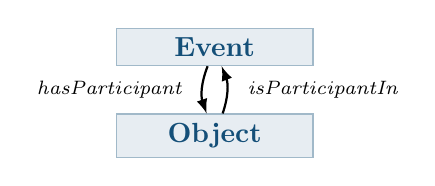
\begin{tikzpicture}
	    \node[owlclass] (A) {Event};
	    \node[owlclass,below=0.6cm of A] (B) {Object};
	    \draw (A) edge[relationxl] node[midway,label=left:hasParticipant] {} (B);
	    \draw (B) edge[relationxr] node[midway,label=right:isParticipantIn] {} (A);
	\end{tikzpicture}}
	%% Example KnowRob language expressions
	\ODPEXAMPLES{
		\emph{has\_participant($x$,$y$)} &
		$y$ is involved in event $x$
	}
\end{ODP}

%\textbf{todo: Sascha write this}
Agents are defined as \emph{agentive objects, either physical (e.g. a robot, a human or a whale) or social (e.g. a corporation, an institution or a community)}, Actions are defined as events with \emph{at least one agent that is participating in it, and that is executing a task}. An example would be an robot that is grasping an object. In that case the robot is the agent and grasping would be the a task executed in an action. Actions can be executed by multiple agents. 

\begin{ODP}{Action Execution}
	\ODPINTENT{To represent that an agent has executed an action.}
	\ODPDEFINEDIN{SOMA.owl}
	\ODPQUESTION{Which agent did execute this action? Which actions are executed by this agent?}
	\ODPGRAPHIC{
	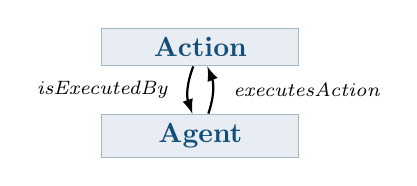
\begin{tikzpicture}
	    \node[owlclass] (A) {Action};
	    \node[owlclass,below=0.6cm of A] (B) {Agent};
	    \draw (A) edge[relationxl] node[midway,label=left:isExecutedBy] {} (B);
	    \draw (B) edge[relationxr] node[midway,label=right:executesAction] {} (A);
	\end{tikzpicture}
	}
	%% Example KnowRob language expressions
	\ODPEXAMPLES{
		\emph{is\_executed\_by($x$,$y$)} &
		$y$ is executed by $x$
	}
\end{ODP}

% % % % % % % % % % % % % % % % %
% % % % % % % % % % % % % % % % %
\subsubsection{Composition}
\label{sec:composition}

%\textbf{todo: Mihai write this.}
%\textbf{todo: why isn't hasPhase Event-to-Event?}

Because an Entity \todo{Seba: What is an Entity ? Is this an object?} often has relevant internal structure, it is necessary to represent relations between it and the other entities that make up its composition. DUL provides two such structuring relations: \emph{hasConstituent} and \emph{hasPart}. We will focus on \emph{hasPart} in this section, but we will briefly discuss the difference between the two relations as well. \todo{Seba: Why only hasPart ?}

The \emph{hasConstituent} relation is intended to connect entities from different ontological layers or levels of abstraction of looking at the world. A material is a constituent of the object it makes up; individual persons are constituents of a corporation. While these constituency relations could often be in colloquial language described as parthood, DUL reserves parthood for more restrictive connections between entities closer to each other in their ontological characterization. For example, a corporation is a \emph{SocialObject} and as such can only have \emph{SocialObjects} as parts, whereas human persons are \emph{PhysicalAgents}, disjoint from \emph{SocialObjects}.

The \emph{hasPart} relation is transitive and defined to have domain and range \emph{Entity}, that is, in principle it could link entities from any concepts together. However, various concepts restrict what can be parts of their instances as exemplified above; as another example, \emph{PhysicalObjects} can only have other \emph{PhysicalObjects} as parts. In SOMA, we define more specialized subproperties of \emph{hasPart} to deal with parts of \emph{Events} vs. parts of \emph{Objects}. The relevant properties are \emph{hasPhase} and \emph{hasComponent} respectively; both are subproperties of \emph{hasPart}.

\begin{ODP}{Event Phases}
	\ODPINTENT{To represent how an event is composed of phases.}
	\ODPDEFINEDIN{SOMA.owl}
	\ODPQUESTION{What are the phases of this action? Is this a phase of some action?}
	\ODPGRAPHIC{
	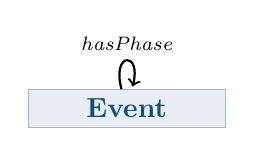
\begin{tikzpicture}
	    \node[owlclass] (E) {Event};
	    \path (E) edge[relation,loop above] node {hasPhase} (E);
	\end{tikzpicture}
	}
	%% Example KnowRob language expressions
	\ODPEXAMPLES{
		\emph{has\_phase($x$,$y$)} &
		$y$ is a phase of $x$
	}
\end{ODP}

%\lipsum[2]

\begin{ODP}{Composition}
	\ODPINTENT{To represent proper parthood of objects.}
	\ODPDEFINEDIN{DUL.owl}
	\ODPQUESTION{What is this object component of? What are the components of this object?}
	\ODPGRAPHIC{
	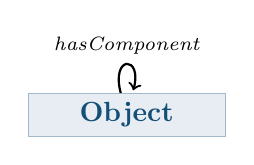
\begin{tikzpicture}
	    \node[owlclass] (E) {Object};
	    \path (E) edge[relation,loop above] node {hasComponent} (E);
	\end{tikzpicture}
	}
	%% Example KnowRob language expressions
	\ODPEXAMPLES{
		\emph{has\_component($x$,$y$)} &
		$y$ is a proper part of $x$
	}
\end{ODP}

\todo{Seba: For me this section makes sense. However, I have the feeling that compared to the previous sections, this section requires maybe more knowledge in ontologies to be understand. Maybe we should give it to someone how does not have any knowledge about ontologies.}

\todo{Daniel: I agree, probably we do not need to discuss the distinction between hasConstituent and hasPart here as it does not help the people to generate neems. We should limit to what is necessary here.}

% % % % % % % % % % % % % % % % %
% % % % % % % % % % % % % % % % %
\subsubsection{Conceptual Classification}
\label{sec:classification}

The classification of entities is done from multiple viewpoints.
The most essential one is \emph{what the entitiy really is}.
This is reflected in the taxonomy.
However, entities may further be classified according to social aspects such as intention, purpose, etc.
This type of classification is based on the \emph{conceptualization} of entities.
In particular, conceptualizations of objects and events are used to classify them in the scope of some activity.
For this purpose,
a comprehensive collection of concepts is used to classify objects and events from a conceptual viewpoint (\textbf{todo: insert link to list of all concepts}).

An object that participates in an event usually plays a certain role during the event.
Some objects are designed to be used in certain ways, thus playing certain roles in specific tasks.
This is, for example, a box which is designed to be used as a container to store items.
However, roles may also be taken by objects that are not designed to be used as such.
The box could, for example, also be used as a door stopper, but surely it would be
inappropriate to classify it as such taxonomically.
Instead, roles are defined as concepts that are used to classify the objects that particpate in an event from a conceptual viewpoint.

\begin{ODP}{Object Role}
	\ODPINTENT{To represents objects and the roles they play.}
	\ODPDEFINEDIN{DUL.owl}
	\ODPQUESTION{What role does this object play? Which objects do play that role?}
	\ODPGRAPHIC{
	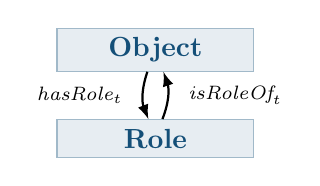
\begin{tikzpicture}
	    \node[owlclass] (A) {Object};
	    \node[owlclass,below=0.6cm of A] (B) {Role};
	    \draw (A) edge[relationxl] node[midway,label=left:$\text{hasRole}_t$] {} (B);
	    \draw (B) edge[relationxr] node[midway,label=right:$\text{isRoleOf}_t$] {} (A);
	\end{tikzpicture}
	}
	%% Example KnowRob language expressions
	\ODPEXAMPLES{
		\emph{has\_role($x$,$y$)} &
		$y$ is a role of $x$ \\
		% % % % %
		\emph{has\_role($x$,$y$) during $z$} &
		$y$ is a role of $x$ during the occurrence of $z$
	}
\end{ODP}

The conceptualization of an event is about how it should be interpreted, executed, expected, seen, etc.
One aspect is that a single event may contribute to multiple goals, such as when an ingredient is fetched that is partly used in a step of a cooking recipe, and partly eaten raw to satisfy hunger.
In such a case, the taxonomical category of the event would be unclear in case it should describe the goal to which the event contributes.
Another aspect is that intentions of agents may not always be known such that the classification of events based on their goals is difficult, and different viewpoints on the same event may exist.
Hence, when referring to goals, intentions, etc. we rather employ conceptual classification.
This allows us to represent several different classifications of the same event in one or more situational contexts, for example an interpretations of the same event from different viewpoints.
%\todo{Seba: How the conceptualization of an event looks in the end? Do we have only one classification or can it have multiple classifications if the goal is not clear?}

\begin{ODP}{??}
	\ODPINTENT{To represent how events should be interpreted, executed, expected, seen, etc.}
	\ODPDEFINEDIN{SOMA.owl}
	\ODPQUESTION{What are the events that are classified by this concept? What are the concepts that classify this event?}
	\ODPGRAPHIC{
	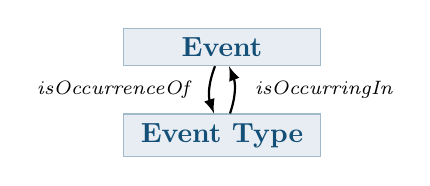
\begin{tikzpicture}
	    \node[owlclass] (A) {Event};
	    \node[owlclass,below=0.6cm of A] (B) {Event Type};
	    \draw (A) edge[relationxl] node[midway,label=left:isOccurrenceOf] {} (B);
	    \draw (B) edge[relationxr] node[midway,label=right:isOccurringIn] {} (A);
	\end{tikzpicture}
	}
	%% Example KnowRob language expressions
	\ODPEXAMPLES{
		\emph{is\_occurring\_in($x$,$y$)} &
		$y$ is an occurrence that is classified by $x$ \\
		% % % % %
		\emph{is\_executed\_in($x$,$y$)} &
		$y$ is an action that executes the task $x$
	}
\end{ODP}

%This ODP allows to make assertions on roles played by agents without involving the agents that play that roles, and vice versa. It allows to express neither the context type in which tasks are defined, not the particular context in which the action is carried out. Moreover, it does not allow to express the time at which the task is executed through the action (for actions that do not solely execute that certain task).
%\lipsum[2]

%\begin{ODP}{Task Execution}
%	\ODPINTENT{To represent actions through which tasks are executed.}
%	\ODPDEFINEDIN{DUL.owl}
%	\ODPQUESTION{Which task is executed through this action? What actions could execute that task?}
%	\ODPGRAPHIC{
%	\begin{tikzpicture}
%	    \node[owlclass] (A) {Action};
%	    \node[owlclass,below=0.6cm of EVT] (B) {Task};
%	    \draw (A) edge[relationxl] node[midway,label=left:executesTask] {} (B);
%	    \draw (B) edge[relationxr] node[midway,label=right:isExecutedIn] {} (A);
%	\end{tikzpicture}
%	}
%	%% Example KnowRob language expressions
%	\ODPEXAMPLES{
%		\emph{??} &
%		??
%	}
%\end{ODP}

% % % % % % % % % % % % % % % % %
% % % % % % % % % % % % % % % % %
\subsubsection{Object Transformation}
\label{sec:transformation}

Objects typically undergo changes by taking part in actions or processes. Such changes typically take one of two forms: either some property of an object changes value, or the object itself modifies its ontological characterization. As an example, a wad of dough being transported from the table to the inside of an oven has changed its position, but is still, at this point, a wad of dough. Left in a hot oven for enough time however, the wad of dough becomes bread.

The variation with time of object qualities has been described in section~\ref{sec:qualification}. The object transformation pattern, described here, handles the changes of an object's ontological classification through time. An immediate problem is that ontological characterizations are necessarily discrete -- there is a finite number of classes an object can belong to -- while change in the physical world is continuous. In the example above, the wad of dough ceases to be dough after a few moments in the oven, because its chemical composition is changing away from the composition of dough. Nonetheless, it is not bread yet.

For practical purposes however, human beings often do not care about the exact classification of an object undergoing ontological change; only the endpoints are important. Also, there is a tendency to loosely apply ontological classification to the changing object, as if it were on either side of the transformation. The cooking wad of dough could be referred to as dough, or it could be referred to as bread. It is both, and neither. While sufficient for causal discourse, such carelessness would not work in a formal system. Hence, the approach in SOMA is to define a class of objects called \emph{Transient}, and it is to this class that objects undergoing ontological classification change belong to. A Transient \emph{transitionsFrom} some object with a specific classification (e.g. \emph{Dough}) and \emph{transitionsTo} another object with a specific classification (e.g. \emph{Bread}). These two relations can be combined into the \emph{transitionsBack} relation, to cover situations where an object changes in essential ways during an event, but returns to being itself after the event completes, such as a catalyst in a chemical reaction.
 
% This pattern addresses the fact that objects change by undergoing/taking part in Processes. For example, the PancakeMix becomes, through Baking, a Pancake. However, the ontological status of the object while the process takes place is unclear: the object placed on the frying pan is not a Pancake until Baking finishes, but it's not PancakeMix either once it begins to coagulate. In the EASE approach, the object in-between such characterizations is a Transient. A Transient transitionsFrom an Object, and possibly transitionsTo an Object. It may also be the case that a Transient transitionsBack to an Object, to indicate that once the process completes, the same Object is restored; this would be the case for example for catalysts in chemistry, or a loaf of bread after slicing, if there is enough bread left.
%\lipsum[2]

\begin{ODP}{Transient}
	\ODPINTENT{Ontological classification for objects undergoing type changes.}
	\ODPDEFINEDIN{SOMA.owl}
	\ODPQUESTION{What sort of object is this? What objects ``went'' into the making of another? What is the outcome of some process of change acting on an object? Does an object preserve or restore its identity after change?}
	\ODPGRAPHIC{
	\begin{tikzpicture}
 %\node[owlclass] (TRANSIENT) {
 %\begin{owlclass}{Transient}
 % \item \texttt{Object}
 % \item $(\exists\emph{transitionsFrom}.\texttt{Object})$
 % \item $(\forall\emph{transitionsTo}.\texttt{Object})$
 %\end{owlclass}
 %};
 %\node[owlclass,below=0.6cm of TRANSIENT] (TRANSITIONSBACK) {
 %\begin{owlclass}{transitionsBack}
 % \item \texttt{transitionsFrom}
 % \item \texttt{transitionsTo}
 %\end{owlclass}
 %};
	    \node[owlclass] (A) {Transient};
	    \node[owlclass,below=0.6cm of A] (B) {Object};
	    \node[owlclass,above=0.6cm of A] (C) {Object};
	    \draw (A) edge[relation] node[midway,label=right:transitionsFrom] {} (B);
	    \draw (A) edge[relation] node[midway,label=right:transitionsTo] {} (C);
	\end{tikzpicture}
	}
	%% Example KnowRob language expressions
	\ODPEXAMPLES{
		\emph{transitionsFrom('A','B')} & By entering some process of change, object 'B' becomes Transient object 'A'.\\
		\emph{transitionsTo('A','B')} & By completing some process of change, transient 'A' becomes object 'B'.\\
		\emph{transitionsBack('A','B')} & Object 'B' entered some process of change during which its ontological classification is unclear and it is replaced by Transient 'A', but after the process completes object 'B' is restored.\\
	}
\end{ODP}

% % % % % % % % % % % % % % % % %
% % % % % % % % % % % % % % % % %
\subsubsection{Force Interaction}

\textbf{todo: Daniel write this}
\textbf{todo: preservative vs. alterative interaction}
\textbf{todo: how to represent who is stronger? can measured forces be included in the NEEM?}
\textbf{todo: isProcessTypeOf relation is not nice}
\lipsum[2]

\begin{ODP}{?}
	\ODPINTENT{To represent force dynamical event characteristics.}
	\ODPDEFINEDIN{SOMA.owl}
	\ODPQUESTION{What entity is the agonist in this event? What are the events where this entity is an antagonist? Which entity is stronger in this event? What is the force dynamical tendency in this event?}
	\ODPGRAPHIC{
	\begin{tikzpicture}
	    \node[owlclass] (A) {Event};
	    \node[owlclass,below=0.6cm of A] (B) {Object};
	    \node[owlclass,below=0.6cm of B,xshift=-1.3cm] (C) {Agonist};
	    \node[owlclass,below=0.6cm of B,xshift=1.3cm]  (D) {Antagonist};
	    \node[owlclass_f,above=0.6cm of A,xshift=-1.3cm] (E) {Alterative Interaction};
	    \node[owlclass_f,above=0.6cm of A,xshift=1.3cm]  (F) {Preservative Interaction};
	    \draw (B) edge[relation] node[midway,label=left:$\text{hasRole}_t$] {} (C);
	    \draw (B) edge[relation] node[midway,label=right:$\text{hasRole}_t$] {} (D);
	    \draw (A) edge[relation] node[midway,label=left:$\text{isOccurrenceOf}$] {} (E);
	    \draw (A) edge[relation] node[midway,label=right:$\text{isOccurrenceOf}$] {} (F);
	    \draw (A) edge[relationxl] node[midway,label=left:hasWeakerEntitiy] {} (B);
	    \draw (A) edge[relationxr] node[midway,label=right:hasStrongerEntitiy] {} (B);
	\end{tikzpicture}
	}
	%% Example KnowRob language expressions
	\ODPEXAMPLES{
		\emph{??} & ??
	}
\end{ODP}

\lipsum[2]

\begin{ODP}{?}
	\ODPINTENT{To quantify force dynamical event characteristics.}
	\ODPDEFINEDIN{SOMA.owl}
	\ODPQUESTION{What is the effort of the agonist in this event?}
	\ODPGRAPHIC{
	\begin{tikzpicture}
	    \node[owlclass] (B) {Force Interaction};
	    \node[owlclass,below=0.6cm of B,xshift=-1.3cm] (C) {Resultant};
	    \node[owlclass,below=0.6cm of C] (D) {Effort};
	    \node[data,right=0.6cm of D] (E) {$Nm$};
	    \draw (B) edge[relation] node[midway,label=right:xx] {} (C);
	    \draw (C) edge[relation] node[midway,label=right:xx] {} (D);
	    \draw (D) edge[relation] node[midway,label=above:xx] {} (E);
	\end{tikzpicture}
	}
	%% Example KnowRob language expressions
	\ODPEXAMPLES{
		\emph{??} & ??
	}
\end{ODP}

% % % % % % % % % % % % % % % % %
% % % % % % % % % % % % % % % % %
\subsubsection{Episodes}
\label{sec:episodes}

An episode is seen as a \emph{relational context} created by an observer that creates a view on a set of entities such as actions that were perfomed, and objects that played a role. We say that an episode is a \emph{setting for} each entity that is relevant for the scope of the episode. As an example, consider the statement \emph{"this morning the robot made a mess on the floor while preparing coffee"}, where the preparation of coffee in the morning is the setting for the robot, the floor, and the actions that were perfomed.
Several specializations of the general \emph{is setting for} relation exist that can be used to distinguish between entities based on their type -- these are, among others, \emph{includesObject} and \emph{includesAgent}.
However, assuming hierachical organization of objects (i.e. all objects are part of some map), and events (i.e. an event is composed into sub-events) only those entities at the root of the composition (e.g. the map) are required to be included explicitely in the episode.

\begin{ODP}{isSettingFor}
	\ODPINTENT{To represent that entites are included in a situation.}
	\ODPDEFINEDIN{DUL.owl}
	\ODPQUESTION{What are the entities that are relevant for this situation? What are the situations where this entity is relevant?}
	\ODPGRAPHIC{
	\begin{tikzpicture}
	    \node[owlclass] (A) {Situation};
	    \node[owlclass,below=0.6cm of A] (B) {Entity};
	    \draw (A) edge[relationxl] node[midway,label=left:isSettingFor] {} (B);
	    \draw (B) edge[relationxr] node[midway,label=right:hasSetting] {} (A);
	    hasSetting
	\end{tikzpicture}
	}
	%% Example KnowRob language expressions
	\ODPEXAMPLES{
		\emph{is\_setting\_for($x$,$y$)} &
		$x$ is a setting for $y$
	}
\end{ODP}

Episodes refer to concrete occurences with actual objects that are involved, and actual events that occur.
The conceptualization of an episode is an abstraction that refers to concepts instead that are used to classify entities that are included in the episode.
Such conceptualizations are called \emph{descriptions}.
We say that an episode \emph{satisfies} a description in case the view represented
by the episode is consistent with the conceptualization given by the description.
Diagnosis being one example of a description of an episode.
Stating that the performance of the robot was \emph{amateurish} when it made a mess on the floor while
preparing coffee is one example for describing an epsiode.
Another type of descriptions are plans that are used to conceptualize the structure of an activity.

\begin{ODP}{satisfies}
	\ODPINTENT{To represent a conceptualization of a situation.}
	\ODPDEFINEDIN{DUL.owl}
	\ODPQUESTION{How can this situation be conceptualized? What are the situations that are consitent with this conceptualization?}
	\ODPGRAPHIC{
	\begin{tikzpicture}
	    \node[owlclass] (A) {Situation};
	    \node[owlclass,below=0.6cm of A] (B) {Description};
	    \draw (A) edge[relationxl] node[midway,label=left:satisfies] {} (B);
	    \draw (B) edge[relationxr] node[midway,label=right:isSatisfiedBy] {} (A);
	\end{tikzpicture}
	}
	%% Example KnowRob language expressions
	\ODPEXAMPLES{
		\emph{satisfies($x$,$y$)} &
		$x$ is consistent with $y$
	}
\end{ODP}

% % % % % % % % % % % % % % % % %
% % % % % % % % % % % % % % % % %
% % % % % % % % % % % % % % % % %
% % % % % % % % % % % % % % % % %
% % % % % % % % % % % % % % % % %
% % % % % % % % % % % % % % % % %

\iffalse
\begin{ODP}{Process vs. Action}
%\ODPDESCRIPTION{An Action is an Event with at least one Agent participant, such that this Agent has a Task, often defined by a Plan or Workflow, which it executes through the Action. A Process is an Event for which no such commitments have been made. In DUL, these classes are not disjoint, allowing a particular event individual to be classified as either, depending on whether we care to record an agent and its goals or not. In EASE, we use Process as a top-level class for events with no agentive participant.}
\ODPINTENT{To represent the intentional and agentive structure-- or lack thereof-- behind Events.}
\ODPDEFINEDIN{DUL.owl}
\ODPQUESTION{
  \emph{Is there anyone responsible for the event?}
  \emph{What are they trying to do?}
  \emph{How did an event unfold?}}
\ODPGRAPHIC{
\begin{tikzpicture}
 \node[owlclass] (ACTION) {
 \begin{owlclass}{Action}
  \item \texttt{Event}
  \item $(\exists \emph{hasParticipant}.\texttt{Agent})$
 \end{owlclass}
 };
 \node[owlclass,below=0.6cm of ACTION] (PROCESS) {
 \begin{owlclass}{Process}
  \item \texttt{Event}
 \end{owlclass}
 };
\end{tikzpicture}
}
\end{ODP}

\begin{ODP}{State, Configuration, Gestallt}
%\ODPDESCRIPTION{A state is a configuration of the world that is construed to be stable on its own. Outside disturbances may cause state transitions, and the settling into some other, self-stable configuration. A State is also characterized by a Description, that indicates things such as what kind of entities participate in the state, what relations might exist between them, what regions may be used by particular qualities of the participants. This Description is, in general, referred to as a Configuration, however some common examples are Goals-- describe desired states of the world--, Norms-- describe states that should be kept--, and Diagnoses-- describe a state that causes certain observable symptoms. States are classified by Gestallts. \textbf{TODO}: Generalize this and/or split it: classification by an event type and structuring by a description are different ODPs in the current list. All three event subclasses (Actions, Processes, States) now are each part of their own Event-Concept-Description triad, where the Concept classifies the Event, and the Description, by describing the classifying Concept, structures the Event.
}
\ODPINTENT{Ontological representation for situations in the world that are cognitively construed as stable arrangements of entities.}
\ODPDEFINEDIN{EASE-STATE.owl}
\ODPQUESTION{
  \emph{What are stable arrangements?}
  \emph{What is meant by ``state'' of the world?}
  \emph{What characterizes a state?}}
\emph{Examples}
%\begin{itemize}
%  \item AssemblyConnection: two objects are in a rigid connection, such that the movement of one determines the movement of the other. In this case the characterizing Configuration for this State uses several Roles-- one for each part/geometric feature belonging to the connected objects-- and puts constraints on the relative positioning of these geometric features such that they interlock to produce the rigid connection.
%  \item Contact: two objects are in mechanical contact. The characterizing Configuration uses two Roles, one for each participating object, and puts constraints on the Pose qualities of the participants: the poses should be such that the participants touch.
%  \item FunctionalControl: an object restricts the movement of another, at least partially. The Configuration uses the Roles Item and Restrictor. More concrete examples are Containment: the Restrictor is a Container, and the Pose quality of the Item should use the region inside the Container; and Support: both Restrictor and Item are objects, placed in such a way that the Item does not move because of gravity.
%  \item PhysicallyAccessible: the Configuration for this state uses the roles Item, a Container or Protector, and optionally an Accessor and a Task, and states that an Item is either placed in a Container or protected by a Protector, but the placement of the Item and Container is such that an Accessor may nevertheless reach the Item in order to perform a Task. For a more concrete example, a DoorOpen is a kind of PhysicallyAccessible where the Protector is a door, the Item is the inside of the room behind the door, the Accessor is some person and the Task is to walk into the inside of the room.
%\end{itemize}
\end{ODP}

\begin{ODP}{Designed Artifact}
%\ODPDESCRIPTION{A DesignedArtifact is a physical object described by a Design. In EASE, Designs refer to the form, but also the function of an object. This allows us to say that an object is ``for'' a particular purpose, even though it might be used for something else instead. For example, a cup is a BeverageContainer but can be used as a Flowerpot. Designs form a hierarchy of specificity, for example $DesignMilkContainer \sqsubseteq DesignBeverageContainer \sqsubseteq DesginContainer \sqsubseteq Design$. The justification for this pattern is that the type of an object is rigid, but the roles it plays in events change. A naive taxonomy, without a notion similar to Design, cannot tackle the fact that objects are usable in several ways beyond the obvious; a hammer isn't always a hammer, sometimes it's a paperweight. On the other hand, a usable ontology of objects must take into account how human users refer to objects by their default use.}
\ODPINTENT{To explicate the intuitive classification human users would have of objects, based on their default uses.}
\ODPDEFINEDIN{DUL.owl, EASE.owl, EASE-middle.owl}
\ODPQUESTION{
  \emph{What sort of object is this?}
  \emph{What is the intended use of the object?}
  \emph{How did an event unfold?}}
\ODPGRAPHIC{
\begin{tikzpicture}
 \node[owlclass] (DESIGNEDARTIFACT) {
 \begin{owlclass}{DesignedArtifact}
  \item \texttt{PhysicalArtifact}
  \item $(\exists\emph{isDescribedBy}.\texttt{Design})$
 \end{owlclass}
 };
 \node[owlclass,below=0.6cm of DESIGNEDARTIFACT] (DESIGN) {
 \begin{owlclass}{Design}
  \item \texttt{Description}
 \end{owlclass}
 };
 \draw (DESIGNEDARTIFACT) edge[thick,-,dashed,blue!60] (DESIGN);
\end{tikzpicture}
}
\end{ODP}
\fi

% In version \neemversion the \neemnar consists the belief state and action task hierarchy. 
% In the following sections we will describe how the belief state and action task hierarchy are represented.
% An concrete example for a logged \neemnar will be given in Chapter \ref{ch:example}.

% \subsection{Belief State}
% 
In EASE, we investigate everyday manipulation activities.
These involve the interaction with physical objects such as
grasping an object and putting it somewhere,
or taking a tool and applying it on an object to achieve a certain effect.
To tell a comprehensive story about its activity,
an agent needs to memorize the relation of action to
physical objects that are salient during the action.

One requirement for this is that beliefs of the agent about the existence
of physical objects must be maintained by the system.
In some cases, when the existence is known in advance,
it is sufficient to supply this knowledge to the agent through
a static ontology holding facts about existence of physical objects
in the environment of the agent.
This is, for example, useful to supply knowledge about a static
environment such as a kitchen with fixed set of appliances.
In more dynamic set-ups, however, the beliefs about the existence
of physical objects must be formed through specialized perception
methods, or through logical reasoning.
This is, for example, the case when the particular set of objects
contained in a drawer are unknown in advance.
We consider this type of information as part of the NEEM narrative
to keep these beliefs persistent, and to allow referring to
the perceived objects in action descriptions.

Episodic memories capture information about temporal situations
during which the beliefs of the agent evolve according to
perception, action, and logical inference.
NEEMs capture this evolution of beliefs.
As such, revised or false beliefs are not deleted but kept
persistently as part of the NEEM narrative.
This is to allow for deeper analysis of the agent performance,
and to provide richer input for learning algorithms.
This is realized through a 4D ontology that we describe at
the end of this section.

%%%%%%%%%%%%%%%%%%%%%%%%%%%%%
%%%%%%%%%%%%%%%%%%%%%%%%%%%%%
%%%%%%%%%%%%%%%%%%%%%%%%%%%%%
%%%%%%%%%%%%%%%%%%%%%%%%%%%%%
\subsection{Tangible Objects}
To refer to objects in action descriptions only the name of the 
object must be known to the NEEM acquisition system.
\knowrob comes with a rather comprehensive object type system,
with about XXX different object classes~\cite{knowrob-ontology}.
The type system is represented as part of the TBOX of the knowledge base.
Perceived objects are represented as instance of one of the object types
provided by the \knowrob system.
This type of information is part of the ABOX of the knowledge base.
The name of an object is usually the name of the class followed
by a underscore character and a 8-digit hash,
but could potentially be any unique name string.

\todo{introduce base class of objects, give some details about taxonomy}

In systems relying on sensor information and statistical models one has to deal
with the uncertainty coming from the use of these information sources.
This also affects beliefs about the identity of objects.
The problem of identity resolution can trivially be approached
by computing euclidean distance to known objects.
If the distance is below a certain threshold, it can often be assumed that it is the same object.
Background knowledge can be used to find better estimates for object identity:
An object is inside the gripper as long as it is grasped,
pulled down by gravity to the plane below when the grasp is released again,
and so forth.
Also, the identity of objects is often not so important for decision making,
but rather the properties of the object.
For successfully preparing a slice of bread, for example, any butter will do.
But if there are two butter packages and one is not yet opened one would rather
use the opened one to avoid it getting rancid.
When acquiring NEEMs one has to deal with this identity resolution problem
to allow for referring to objects in the narrative part of the episodic memory.

In the remainder of this section we describe the fundamental binary predicates to
describe physical objects in the belief state.

\begin{description}
\item[\textbf{rdf:type}] 
The most fundamental assertion about an object next to its name is its type.
Types are asserted through the \emph{rdf:type}
property with one of the object types as value.
Ontologies are subsumption hierarchies that derive 
knowledge about more specific concepts from more general concepts.
This allows, for example, to describe the relation between object and action
on a general level that applies to a larger class of objects and actions.
It is further possible to assert multiple types from different branches
of the type hierarchy for a single object.
For example, some mobile phone may also be used as projector while other mobile phones,
without the projector hardware, should not be classified as projector.
%%%%%%%%%%%%%%%%%%%%%%%%%%%%%
%%%%%%%%%%%%%%%%%%%%%%%%%%%%%
\item[\textbf{physicalParts}]
$Whole\ \emph{physicalParts}\ Part$ means
that $Part$ is tangible and one of the distinct parts of the
more complex tangible object $Whole$.
Manipulation is often about putting together parts to form a bigger whole.
During table setting, for example, objects are arranged such that they form
place settings for the different participants.
The objects are placed intentionally such that humans can easily reach them from their seat,
see which objects belong to which place setting, and infer what objects belong to whom.
Another example are assembly tasks during which an agent tries
to put together some mechanical parts using screwing connections, snap-in connection,
and so on to create an assembled product from scattered pieces available.
NEEMs can also represent this partonomy information through dedicated predicates
linking parts to the bigger whole.
In particular, the \ease ontology defines the following sub-properties of \emph{physicalParts}:
\emph{dangerousParts} (e.g., the blade of a knife),
\emph{electricalParts} (i.e., parts that need electrical current to work),
\emph{mealComponents} (i.e., the ingredients of a meal).
%%%%%%%%%%%%%%%%%%%%%%%%%%%%%
%%%%%%%%%%%%%%%%%%%%%%%%%%%%%
\item[\textbf{frameName}] \dots
\end{description}

\todo{some other relevant predicates? shape, color, mesh, pose?}

%%%%%%%%%%%%%%%%%%%%%%%%%%%%%
%%%%%%%%%%%%%%%%%%%%%%%%%%%%%
%%%%%%%%%%%%%%%%%%%%%%%%%%%%%
%%%%%%%%%%%%%%%%%%%%%%%%%%%%%
\subsection{Kinematic Objects}
\begin{enumerate}
 \item \todo{object parts can be connected through joints}
 \item \todo{what types of joints exist?}
 \item \todo{what predicates can be used to describe them?}
\end{enumerate}

%%%%%%%%%%%%%%%%%%%%%%%%%%%%%
%%%%%%%%%%%%%%%%%%%%%%%%%%%%%
%%%%%%%%%%%%%%%%%%%%%%%%%%%%%
%%%%%%%%%%%%%%%%%%%%%%%%%%%%%
\subsection{Environment Maps}
Semantic maps are detailed representations of the environment of some agent.
These include geometrical and visual information about objects and appliances,
their functional decomposition, and their state.
Modern game engines reach an impressive level of detail, with individual
leaves falling down trees, etc.
In EASE, we try to reach this level of detail in our semantic map representations.
We do this to provide very comprehensive information about situated experiences
from which general knowledge can be learned.
We believe that this high level of detail will allow us to learn more robust
models and with less training data then would be possible with
a more abstracted representation of environments.

The \emph{SemanticMap} itself could be a \emph{Room}, a \emph{Building}, or some other type of connected
region in which some agent can do navigation and manipulation.
The ontology defines some more specific room classes including
\emph{Kitchen}, \emph{LivingRoom} and \emph{StoreRoom}.
This is useful, for example, to correlate objects with their likely storage room,
or to relate the rooms with common activities performed in them.

\begin{description}
%%%%%%%%%%%%%%%%%%%%%%%%%%%%%
%%%%%%%%%%%%%%%%%%%%%%%%%%%%%
\item[\textbf{describedInMap}]
$Object\ \emph{describedInMap}\ Map$ means \dots
\end{description}

\todo{also describe how rooms relate to buildings, etc.?}
\todo{something about the state?}


\subsection{Temporal Representation}
\dots

% \subsection{Action Hierarchy}
% \label{ch:narrative,sec:actionHierarchy}
% In this section, we will describe how an action task hierarchy is represented in the \neemnar. 
% Since we are using \cram on our robots our plans do not necessary generate a sequence of actions, instead they will generate rather an hierarchy of actions.
% During the plan execution we are logging all executed actions with its parameters and represent the hierarchy in \owl.
% The general idea of the model is that an action will be represented as an individual of the class \owlClass{knowrob:'Action'}.
% This individual can be a direct instance of the class \owlClass{knowrob:'Action'} or its subclass.
% \todo{Add all supported action sub classes}
% With the predicates \owlPredicate{subAction}, \owlPredicate{previousAction} and \owlPredicate{nextAction}, which all have as subject and object the type \owlClass{knowrob:'Action'}, we are able to represent the action hierarchy.
% In our understanding an logged action hierarchy in an \owl represents all actions which were executed during an experiment.
% Meaning, if we would extracted all actions from the \owl file and recreated the action tree, we would be able to analyze and reasoning about all executed actions during one specific experiment.

% In the next subsections we will describe the predicates and classes which we currently defined in the version \neemversion to log the actions which were executed by the robot during an experiment. 

% \subsection{Action Predicates}
% Every individual of the class \owlClass{knowrob:'Action'} class or its subclass which will be logged in the \owl file can be asserted with the following predicates (see Table \ref{table:action_task_predicates}).
% Some predicates in the table are marked as required.
% This means that if you are intending to upload your \owl file to \openease, every \owlClass{knowrob:'Action'} individual has to have the required properties asserted.
% %Otherwise the \owl file will be revoked from the server.\todo{We have to implement such checking in \openease.}
% The \openease server checks also if the objects of the predicates are associated with the correct class.

% \begin{table}[H]
% 	\begin{tabular}{| c | c | c | c |}
% 		\hline			
% 		\textbf{Subject} & \textbf{Predicate} & \textbf{Object}  & \textbf{Required} \\
% 		\hline
% 		Action & taskSuccess & xsd:boolean & Yes \\
% 		\hline
% 		Action & startTime & Timepoint & Yes \\
% 		\hline
% 		Action & endTime & Timepoint  & Yes \\
% 		\hline
% 		Action & subAction & Action & No \\
% 		\hline
% 		Action & nextAction & Action & No \\
% 		\hline
% 		Action & previousAction & Action & No \\
% 		\hline
% 	\end{tabular}
% 	\caption{Action Predicates}
% 	\label{table:action_task_predicates}
% \end{table}

% \begin{description}
% 	\item[\textbf{taskSuccess}] 
% 		This predicates points to data type \owlClass{xsd:boolean}.
% 		The value \textbf{true} represents that the action was executed successfully.
% 		If any errors occurred during the action execution, the data type will be set to \textbf{false}.
% 		\footnote{In the NEEM version \neemversion we do not log the exact error which happened during action.}
% 	\item[\textbf{startTime}]
% 		The \owlPredicate{startTime} represents when the action started.
% 		Instead of representing the startTime as a data point, we are creating an instance of the class \owlClass{Timepoint}.
% 		The implemenation is done in that way because it made writing prolog queries much more convenient. 
% 		The name of the individual is representing the exact time when the action started e.g.\ \textit{timepoint\_1523878415038090} which can be understood that the action started 1523878415038090 microseconds after 00:00:00 UTC, Thursday, 1 January 1970.
% 		We are using the Unix time to represent a time point \cite{matthew2011beginning}.
% 		However, we are considering to measure the time in microseconds.
% 		The reason for this decision is that we also want to create NEEMs in simulation.
% 		However, tasks in simulation can be executed so fast that logging in microseconds allowed to measure the performance of the task executions.
% 		Also the measurement in microseconds allowed to differentiate the running time between tasks.
% 	\item[\textbf{endTime}] 
% 		This predicate represents when the action ended.
% 		More information about how we log time points is described in the predicate description \owlPredicate{startTime}.
% 	\item[\textbf{subAction}]
% 		The predicate \owlPredicate{subAction} allows to create parent-child relation between two tasks. In the context of this predicate, the subject is the parent action and the object is the child action.
% 		It is possible that an \owlClass{Action} instance can have multiple \owlPredicate{subAction} predicates which point each to a single child action.
% 	\item[\textbf{nextAction}]
% 		To be able to create an sequential order of actions which where executed on the same hierarchy level, we defined the \owlPredicate{nextAction} predicate.
% 		The subject represents the action which was started first and points to the next sibling actions.
% 		\footnote{In the NEEM version \neemversion we are not differentiate if actions were executed in sequence or in parallel.}
% 	\item[\textbf{previousAction}]
% 		Like in \owlPredicate{previousAction} this predicate is created to create an sequential order between siblings tasks.
% 		However in this case, \owlPredicate{previousAction} connects an \owlClass{Action} instance with the sibling action which was performed previously.
% \end{description}


% \subsection{Action Parameter Predicates}
% 	\label{sec:actionParameterPredicactes}
% 	In general, actions have to have parameters which have to be asserted.
% 	Based on those assertions \cram is able to infer how to perform the task.
% 	For instance, a grasping task will be executed differently when the target object is a spoon compared to when the target object is a bottle.
% 	To understand the logged behavior of the robot better, we are logging to each action the corresponding parameters.
% 	For \cram we are using for our actions a set of predefined parameters.
% 	For example, when an action requires an object every \cram action has parameter name \textit{object} asserted.
% 	During the logging process, we are creating based on the parameter's value an instance of the class \owlClass{Object} and connect this instance with the \owlPredicate{objectActedOn}.
% 	\todo{Ref to belief state when object description is done}
% 	This implementation allows us to use the logger for new actions without the need to extend the logger.
% 	As long the \cram actions will use the predefined parameter names all parameters will be logged without the need to extend the logger.
% 	All predefined parameters are represented by a separated predicates which point to the parameter value which is an individual of the corresponding \owl class.
% 	Table \ref{table:action_parameter_predicates} shows the current parameter predicates which are supported by our NEEM representation.
% 	The design of the action parameter predicates is based on the work with our \pr.
% 	Therefore in the NEEM \neemversion it might be possible that the action parameters cannot be used by everyone in this state.
	 
% \begin{table}[H]
% \begin{tabular}{| c | c | c |}
% 	\hline			
% 	\textbf{Subject} & \textbf{Predicate} & \textbf{Object} \\
% 	\hline			
% 	Action & effort & qudt\#NewtonMeter \\
% 	\hline
%     Action & position & Float \\
%     \hline
% 	Action & arm & Pr2\#Pr2RightArm \\
% 	\hline
% 	Action & bodyPartsUsed & Pr2\#Pr2RightGripper \\
% 	\hline
% 	Action & goalLocation & Pose or Connected Space Region \\
% 	\hline
%     Action & objectActedOn & Object \\
% 	\hline
% 	Action & objectType & Object \\
% 	\hline
% \end{tabular}
% 	\caption{Action Parameter Predicates}
% 	\label{table:action_parameter_predicates}
% \end{table}

% \begin{description}
% 	\item[\textbf{effort}] 
% 		Effort is the grasping force in newton-meters.
% 		To model this we are using the \qudt ontology \footnote{http://qudt.org/}.
% 	\item[\textbf{position}]
% 		We are using this predicate to log the the goal position for the gripper of the \pr.
% 		The \pr accepts a joint angle in RAD to position its gripper.
% 		We decided to use a float data type to model the position to be able to represent more different types of position.
% 		For instance, our \boxy robot uses centimeters to position the gripper.
% 		Therefore with a float representation we are able to log from both robots the position parameter.
% 	\item[\textbf{arm}]
% 		With this predicate we want to log which arm was used to by the robot.
% 		The predicate points to an instance of the specific robot arm class.
% 		For instance, to model that the \pr used a right arm to grasp a bottle we are asserting the \owlPredicate{arm} predicate to an individual of the class \owlClass{Pr2RightArm}\footnote{http://knowrob.org/kb/PR2.owl}.
% 	\item[\textbf{bodyPartsUsed}]
% 		The \owlPredicate{bodyPartsUsed} predicate should represent which body part from the robot was used to perform the task.
% 		This predicate can be used \eg to represent that a gripper was used to perform the task.
% 		Like in \dots we also want to represent the body part as instance of the class which represents the body part.
% 	\item[\textbf{goalLocation}]
% 		This predicate can be used to represent the target or location parameter of an action.
% 		This predicate is suitable to represent \eg the target location of an \textit{Going} action.
% 		We are considering to different object types to log the goal location.
% 		Since our robots are build on \ros our robots can work with \textit{Poses} \footnote{http://docs.ros.org/api/geometry\_msgs/html/msg/Pose.html}.
% 		How we represent this \owl class is stated out in section \ref{sec:pose}.
		
% 		Since we are also using \cram, our robots can also encounter \textit{location designator} as goal locations\cite{beetz2010cram}.
% 		That means \cram can handle tasks like "Go to the kitchen counter".
% 		Since locations designators are more abstract we use the \owl class \owlClass{Connected Space Region} to log them.
% 		A more detailed description is given in section \ref{sec:connectedSpaceRegion}.
		
% 	\item[\textbf{objectActedOn}]
% 		With the predicate \owlClass{objectActedOn} we want to log which objects are given as parameter to the action.
% 		For instance, we can log which objects the robots looked for during a perception task and what objects he tried to grab.
% 	\item[\textbf{objectType}]
% 		The difference of \owlPredicate{objectType} compared to \owlPredicate{objectActedOn} is that \owlPredicate{objectType} define not a specific object but rather an object in general.
% 		For instance, if the robotic agent will get a task such as "grab the milk from the fridge".
% 		Given the task, the agent knows only that it has to grab a object of the type of milk from the fridge.
% 		So at this moment the robot does not know if the a milk box is actually in the fridge.
% 		Thereofre it has to recognize the milk first.
% 		If this was sucessfull then the robot will assoicated the following task the milk ID with the predicate \owlPredicate{objectActedOn} which the object will be the link to the speicifc object in the belieft state.
% \end{description}

% \subsection{Action Parameter Classes}
% As shown in section \ref{sec:actionParameterPredicactes} we are not only using data types to log the action parameter.
% In this section we are describing the \owl classes which we introduced to be able to log all parameters which we required to log during our experiments.

% \subsubsection{Pose}
% 	\label{sec:pose}
% 	This class is used to log coordinates given as parameter.
% 	Since our robots are using \ros we are logging poses.
% 	A pose consists from a Quaternion and a 3D vector.
% 	Since both together can only describe a Pose, both entities are required to be logged.
% 	\begin{table}[H]
% 		\begin{tabular}{| c | c | c | c |}
% 			\hline			
% 			\textbf{Subject} & \textbf{Predicate} & \textbf{Object} & \textbf{Required}\\
% 			\hline
% 			Pose & quaternion & String & Yes \\
% 			\hline
% 			Pose & translation & String & Yes \\			
% 			\hline
% 		\end{tabular}
% 		\caption{Pose Predicates}
% 		\label{table:pose_predicates}
% 	\end{table}
	
% 	\begin{description}
% 		\item[Quaternion] 
% 			%Quaternions are used to describe rotations in a three dimensionally space. \todo{Set reference to a Quaternions description}
% 			In the NEEM version \neemversion we are representing quaternions as a string.
% 			For instance, the quaternion $0.5 + 0.35i + 1j +0k$ will be represented as "0.5 0.35 1 0".
% 		\item[Translation]
% 			The \owlClass{Translation} class represents the 3D vector part of the pose.
% 			In the NEEM version \neemversion we are representing vectors as a string.
% 			For instance, the vector $\begin{bmatrix} -0.759, 1.19, 0.932 \end{bmatrix}^T$ will be represented as "-0.759 1.19 0.932".
			
			



% 	\end{description}
	
	
	
% \subsubsection{Connected Space Region}
% 	\label{sec:connectedSpaceRegion}
% 	Since we are using \cram our robots are allowed to use location designators to describe location parameters which will be resolved to pose \cite{beetz2010cram}
% 	The resolving process is divided in three stages:
% 		\begin{enumerate}
% 			\item Define a abstract location or general location. For instance, "Grab the milk from the fridge.".
% 			\item \cram will try out to resolve "fridge" to an entity of the semantic map.
% 			\item The last step is to resolve the entity from the semantic map into a pose with which the robot can actually work with.
% 		\end{enumerate}
	
% 	\begin{table}[H]
% 		\begin{tabular}{| c | c | c | c |}
% 			\hline			
% 			\textbf{Subject} & \textbf{Predicate} & \textbf{Object} & \textbf{Required}\\
% 			\hline
% 			Connected Space Region & onPhysical & iai-kitchen & No \\
% 			\hline
% 		\end{tabular}
% 		\caption{Connected Space Region Predicates}
% 		\label{table:connected_space_region_predicates}
% 	\end{table}
	
% 	\begin{description}
% 		\item[onPhysical] 
% 			To be able to represent the resolution to an entity of the semantic map we defined the \owlPredicate{onPhysical} predicate.
% 			This predicate points to an instance of semantic map.
% 			For instance, to grasp an object from the kitchen counter in our kitchen we link the \owlClass{ConnectedSpaceRegion} instance to an individual of our semantic mal in this case \textit{knowrob:iai\_kitchen\_sink\_area\_counter\_top}.
% 	\end{description}

% \subsubsection{Timepoint}
% 	In the NEEM version \neemversion the \owlClass{Timepoint} does not have any predicates.
% 	An instance of the \owlClass{Timepoint} class defines a moment in time which is represented in microseconds.
% 	The exact timestamp in microseconds is represent in the name of the instance.
% 	For example, the individual with the name "timepoint\_1523878419.243441" represents a timepoint which is 1523878419243441 microseconds after 00:00:00 UTC, Thursday, 1 January 1970.
% 	We are using the Unix time to represent a time point\cite{matthew2011beginning}.
% 	This Timepoint represenation makes the prolog quering much more easier.

% 
% % % % % % % % % % % % % % % % % % % % % % % %
% % % Prelude
% % % % % % % % % % % % % % % % % % % % % % % %
\newcommand{\givenODPNAME}{}
\newcommand{\givenODPINTENT}{}
\newcommand{\givenODPDEFINEDIN}{}
\newcommand{\givenODPDESCRIPTION}{}
\newcommand{\givenODPGRAPHIC}{}
\newcommand{\givenODPDOMAIN}{}
\newcommand{\givenODPQUESTION}{}
\newcommand{\ODPINTENT}[1]     {\renewcommand{\givenODPINTENT}{#1}}
\newcommand{\ODPDEFINEDIN}[1]  {\renewcommand{\givenODPDEFINEDIN}{#1}}
\newcommand{\ODPDESCRIPTION}[1]{\renewcommand{\givenODPDESCRIPTION}{#1}}
\newcommand{\ODPGRAPHIC}[1]    {\renewcommand{\givenODPGRAPHIC}{#1}}
\newcommand{\ODPDOMAIN}[1]     {\renewcommand{\givenODPDOMAIN}{#1}}
\newcommand{\ODPQUESTION}[1]   {\renewcommand{\givenODPQUESTION}{#1}}
\newcommand{\OPDinit}{
  \renewcommand{\givenODPINTENT}{REQUIRED!}
  \renewcommand{\givenODPDEFINEDIN}{REQUIRED!}
  \renewcommand{\givenODPDESCRIPTION}{REQUIRED!}
  \renewcommand{\givenODPGRAPHIC}{REQUIRED!}
  \renewcommand{\givenODPQUESTION}{}
  \renewcommand{\givenODPDOMAIN}{}
  \renewcommand{\labelitemi}{$\mathbf{\sqsubseteq}$}
}

\newenvironment{owlclass}[2][,] {
  \begin{minipage}{5.0cm}
  \begin{center}
  \texttt{\bf#2} \\[-0.2cm]
  \par\noindent\rule{\textwidth}{0.4pt}
  \vspace{-0.6cm}
  \begin{itemize}[#1]
  \raggedright} {
  % % % % % %
  \end{itemize}
  \end{center}
  \end{minipage}
}

\newenvironment{ODP}[1]{
\OPDinit
\renewcommand{\givenODPNAME}{#1}
}{
\givenODPDESCRIPTION
\begin{figure}[htb]
\begin{minipage}{0.45\textwidth}
\begin{tabular}{ p{1.8cm} p{3.2cm} }
\toprule
% {\it\bf Name}                 & \emph{\givenODPNAME} \\
{\it\bf Intent}               & \givenODPINTENT \\
{\it\bf Domains}              & \givenODPDOMAIN \\
{\it\bf Competency Questions} & \givenODPQUESTION \\
{\it\bf Defined in}           & \givenODPDEFINEDIN \\
\bottomrule
\end{tabular}
\end{minipage}
\begin{minipage}{0.55\textwidth}
\begin{center}
\givenODPGRAPHIC
\end{center}
\end{minipage}
\caption{The \emph{\givenODPNAME} ODP.}
\end{figure}
}

\tikzset{owlclass/.style={draw=blue!40,fill=blue!20,rounded corners}}

% % % % % % % % % % % % % % % % % % % % % % % %
% % % % % % % % % % % % % % % % % % % % % % % %
% % % % % % % % % % % % % % % % % % % % % % % %
\chapter{Ontology Design Patterns (ODPs)}

% % % % % % % % % % % % % % % % % % % % % % % %
% \section{Object Roles}

% % % % % % % % % % % % % % % % % % % % % % % %
% % % % % % % % % % % % % % % % % % % % % % % %
% \section{Quality and Quality Regions}

% % % % % % % % % % % % % % % % % % % % % % % %
% % % % % % % % % % % % % % % % % % % % % % % %
% \section{Designed Artifacts}

% % % % % % % % % % % % % % % % % % % % % % % %
% % % % % % % % % % % % % % % % % % % % % % % %
\section{Task Execution ODP}
\begin{ODP}{Task Execution}
\ODPDESCRIPTION{
This ODP allows to make assertions on roles played by agents
without involving the agents that play that roles, and vice versa.
It allows to express neither the context type in which tasks are defined,
not the particular context in which the action is carried out.
Moreover, it does not allow to express the time at which
the task is executed through the action
(for actions that do not solely execute that certain task).}
\ODPINTENT{To represent actions through which tasks are executed. }
\ODPDOMAIN{
  \texttt{Organization},
  \texttt{Management},
  \texttt{Scheduling},
  \texttt{Workflow}}
\ODPDEFINEDIN{DUL.owl}
\ODPQUESTION{
  \emph{Which task is executed through this action?}
  \emph{What actions can execute that task?}}
\ODPGRAPHIC{
\begin{tikzpicture}
 \node[owlclass] (ACTION) {
 \begin{owlclass}{Action}
  \item $(\geq 1\ \emph{executesTask}.\texttt{Task})$
 \end{owlclass}
 };
 \node[owlclass,below=0.6cm of ACTION] (TASK) {
 \begin{owlclass}{Task}
  \item $(\forall \emph{isExecutedIn}.\texttt{Action})$
 \end{owlclass}
 };
 \draw (ACTION) edge[thick,-,dashed,blue!60] (TASK);
\end{tikzpicture}
}
\end{ODP}

\newpage
\section{Quality -- Region ODP}
\begin{ODP}{Quality -- Region}
\ODPDESCRIPTION{This ODP allows structuring information about the properties of an Entity. It distinguishes between dependent aspects of the Entity (things that cannot exist without the Entity itself existing), and the values that may be ascribed to those aspects. These values may be points in some Region. Note that a Region may be a finite set of discrete labels, allowing for ``qualitative'' descriptions, but more often a Region is some dimensional space allowing ``quantitative'' descriptions. A Region may contain a single point, in cases where the value of a Quality is known precisely.}
\ODPINTENT{To distinguish between an aspect of an Entity and a particular numerical description of it.}
\ODPDOMAIN{
  \texttt{Measurement},
  \texttt{Object representation},
  \texttt{Environment representation},
  \texttt{Execution status}}
\ODPDEFINEDIN{DUL.owl}
\ODPQUESTION{
  \emph{What qualities does an entity have?}
  \emph{What are possible values for a quality?}
  \emph{What is the actual value of a quality for a particular entity (at a particular time)?}}
\ODPGRAPHIC{
\begin{tikzpicture}
 \node[owlclass] (QUALITY) {
 \begin{owlclass}{Quality}
  \item $(\exists \emph{isQualityOf}.\texttt{Entity})$
  \item $(\exists \emph{hasRegion}.\texttt{Region})$
 \end{owlclass}
 };
 \node[owlclass,below=0.6cm of QUALITY] (REGION) {
 \begin{owlclass}{Region}
  \item $(\exists \emph{isRegionFor}.\texttt{Quality})$
 \end{owlclass}
 };
 \draw (QUALITY) edge[thick,-,dashed,blue!60] (REGION);
\end{tikzpicture}
}
\end{ODP}

\newpage
\section{Process vs. Action ODP}
\begin{ODP}{Process vs. Action}
\ODPDESCRIPTION{An Action is an Event with at least one Agent participant, such that this Agent has a Task, often defined by a Plan or Workflow, which it executes through the Action. A Process is an Event for which no such commitments have been made. In DUL, these classes are not disjoint, allowing a particular event individual to be classified as either, depending on whether we care to record an agent and its goals or not. In EASE, we use Process as a top-level class for events with no agentive participant.}
\ODPINTENT{To represent the intentional and agentive structure-- or lack thereof-- behind Events.}
\ODPDOMAIN{
  \texttt{Event classification},
  \texttt{Event narratives}}
\ODPDEFINEDIN{DUL.owl}
\ODPQUESTION{
  \emph{Is there anyone responsible for the event?}
  \emph{What are they trying to do?}
  \emph{How did an event unfold?}}
\ODPGRAPHIC{
\begin{tikzpicture}
 \node[owlclass] (Action) {
 \begin{owlclass}{Action}
  \item \texttt{Event}
  \item $(\exists \emph{hasParticipant}.\texttt{Agent})$
 \end{owlclass}
 };
 \node[owlclass,below=0.6cm of ACTION] (PROCESS) {
 \begin{owlclass}{Process}
  \item \texttt{Event}
 \end{owlclass}
 };
\end{tikzpicture}
}
\end{ODP}

\newpage
\section{Designed Artifact ODP}
\begin{ODP}{Designed Artifact}
\ODPDESCRIPTION{A DesignedArtifact is a physical object described by a Design. In EASE, Designs refer to the form, but also the function of an object. This allows us to say that an object is ``for'' a particular purpose, even though it might be used for something else instead. For example, a cup is a BeverageContainer but can be used as a Flowerpot. Designs form a hierarchy of specificity, for example $DesignMilkContainer \sqsubseteq DesignBeverageContainer \sqsubseteq DesginContainer \sqsubseteq Design$. The justification for this pattern is that the type of an object is rigid, but the roles it plays in events change. A naive taxonomy, without a notion similar to Design, cannot tackle the fact that objects are usable in several ways beyond the obvious; a hammer isn't always a hammer, sometimes it's a paperweight. On the other hand, a usable ontology of objects must take into account how human users refer to objects by their default use.}
\ODPINTENT{To explicate the intuitive classification human users would have of objects, based on their default uses.}
\ODPDOMAIN{
  \texttt{Object classification},
  \texttt{Event narratives}}
\ODPDEFINEDIN{DUL.owl, EASE.owl, EASE-middle.owl}
\ODPQUESTION{
  \emph{What sort of object is this?}
  \emph{What is the intended use of the object?}
  \emph{How did an event unfold?}}
\ODPGRAPHIC{
\begin{tikzpicture}
 \node[owlclass] (DESIGNEDARTIFACT) {
 \begin{owlclass}{DesignedArtifact}
  \item \texttt{PhysicalArtifact}
  \item $(\exists\emph{isDescribedBy}.\texttt{Design})$
 \end{owlclass}
 };
 \node[owlclass,below=0.6cm of DESIGNEDARTIFACT] (DESIGN) {
 \begin{owlclass}{Design}
  \item \texttt{Description}
 \end{owlclass}
 };
 \draw (DESIGNEDARTIFACT) edge[thick,-,dashed,blue!60] (DESIGN);
\end{tikzpicture}
}
\end{ODP}

\newpage
\section{Transient ODP}
\begin{ODP}{Transient}
\ODPDESCRIPTION{This pattern addresses the fact that objects change by undergoing/taking part in Processes. For example, the PancakeMix becomes, through Baking, a Pancake. However, the ontological status of the object while the process takes place is unclear: the object placed on the frying pan is not a Pancake until Baking finishes, but it's not PancakeMix either once it begins to coagulate. In the EASE approach, the object in-between such characterizations is a Transient. A Transient transitionsFrom an Object, and possibly transitionsTo an Object. It may also be the case that a Transient transitionsBack to an Object, to indicate that once the process completes, the same Object is restored; this would be the case for example for catalysts in chemistry, or a loaf of bread after slicing, if there is enough bread left.}
\ODPINTENT{Ontological classification for objects undergoing type changes.}
\ODPDOMAIN{
  \texttt{Object classification},
  \texttt{Event narratives}}
\ODPDEFINEDIN{EASE.owl, EASE-middle.owl}
\ODPQUESTION{
  \emph{What sort of object is this?}
  \emph{What objects ``went'' in the making of another?}
  \emph{Does an object preserve or restore its identity after change?}}
\ODPGRAPHIC{
\begin{tikzpicture}
 \node[owlclass] (TRANSIENT) {
 \begin{owlclass}{Transient}
  \item \texttt{Object}
  \item $(\exists\emph{transitionsFrom}.\texttt{Object})$
  \item $(\forall\emph{transitionsTo}.\texttt{Object})$
 \end{owlclass}
 };
 \node[owlclass,below=0.6cm of TRANSIENT] (TRANSITIONSBACK) {
 \begin{owlclass}{transitionsBack}
  \item \texttt{transitionsFrom}
  \item \texttt{transitionsTo}
 \end{owlclass}
 };
\end{tikzpicture}
}
\end{ODP}

\newpage
\section{States}
\begin{ODP}{State, Configuration, Gestallt}
\ODPDESCRIPTION{A state is a configuration of the world that is construed to be stable on its own. Outside disturbances may cause state transitions, and the settling into some other, self-stable configuration. A State is also characterized by a Description, that indicates things such as what kind of entities participate in the state, what relations might exist between them, what regions may be used by particular qualities of the participants. This Description is, in general, referred to as Gestallt, however some common examples are Goals-- describe desired states of the world--, Norms-- describe states that should be kept--, and Diagnoses-- describe a state that causes certain observable symptoms.}
\ODPINTENT{Ontological representation for situations in the world that are cognitively construed as stable arrangements of entities.}
\ODPDOMAIN{
  \texttt{Event classification},
  \texttt{Event narratives}}
\ODPDEFINEDIN{EASE.owl, EASE-middle.owl}
\ODPQUESTION{
  \emph{What are stable arrangements?}
  \emph{What is meant by ``state'' of the world?}
  \emph{What characterizes a state?}}
\emph{Examples}
\begin{itemize}
  \item AssemblyConnection: two objects are in a rigid connection, such that the movement of one determines the movement of the other. In this case the characterizing Gestallt for this State uses several Roles-- one for each part/geometric feature belonging to the connected objects-- and puts constraints on the relative positioning of these geometric features such that they interlock to produce the rigid connection.
  \item Contact: two objects are in mechanical contact. The characterizing Gestallt uses two Roles, one for each participating object, and puts constraints on the Pose qualities of the participants: the poses should be such that the participants touch.
  \item FunctionalControl: an object restricts the movement of another, at least partially. The Gestallt uses the Roles Item and Restrictor. More concrete examples are Containment: the Restrictor is a Container, and the Pose quality of the Item should use the region inside the Container; and Support: both Restrictor and Item are objects, placed in such a way that the Item does not move because of gravity.
  \item PhysicallyAccessible: the Gestallt for this state uses the roles Item, a Container or Protector, and optionally an Accessor and a Task, and states that an Item is placed either in a Container or protected by a Protector, but the placement of the Item and Container is such that an Accessor may nevertheless reach the Item in order to perform a Task. For a more concrete example, a DoorOpen is a kind of PhysicallyAccessible where the Protector is a door, the Item is the inside of the room behind the door, the Accessor is some person and the Task is to walk into the inside of the room.
\end{itemize}
%\ODPGRAPHIC{
%\begin{tikzpicture}
% \node[owlclass] (TRANSIENT) {
% \begin{owlclass}{Transient}
%  \item \texttt{Object}
%  \item $(\exists\emph{transitionsFrom}.\texttt{Object})$
%  \item $(\forall\emph{transitionsTo}.\texttt{Object})$
% \end{owlclass}
% };
% \node[owlclass,below=0.6cm of TRANSIENT] (TRANSITIONSBACK) {
% \begin{owlclass}{transitionsBack}
%  \item \texttt{transitionsFrom}
%  \item \texttt{transitionsTo}
% \end{owlclass}
% };
%\end{tikzpicture}
%}
\end{ODP}

% % % % % % % % % % % % % % % % % % % % % % % %
% % % % % % % % % % % % % % % % % % % % % % % %
% \section{Workflows}

% % % % % % % % % % % % % % % % % % % % % % % %
% % % % % % % % % % % % % % % % % % % % % % % %
% \section{Action Phases}

% % % % % % % % % % % % % % % % % % % % % % % %
% % % % % % % % % % % % % % % % % % % % % % % %
% \section{Transients}




% \subsection{Knowledge Bases}

In this chapter we should describe all knowledge bases we are using to represent the NEEMs.

\subsubsection{IAI-Kitchen}
\subsubsection{Knowrob}
\subsubsection{PR2}
\subsubsection{Qudt}



\setcounter{section}{0}
\chapter{NEEM-Experience}

\neemexp captures low-level information about experienced activities
represented as time series data streams.
This data has often no or only unfeasible
lossless representation as facts in a knowledge base.
To make this data \emph{knowledgable}, procedural hooks
are defined in the ontology to compute symbols from the experience data,
and to embed these symbols in logic-based reasoning.

The data is stored in a NoSQL database using JSON documents.
Each individual type of data is stored in a separate collection
named according to the type of data stored in the collection.
When imported, the knowledge system stores the data in a
\mongodb\footnote{https://www.mongodb.com/} server, for which
the knowledge system implements a client for querying the data
during question answering.
The query cursor concept employed in \mongodb integrates
nicely with backtracking based search employed in the knowledge system.
It further scales well to large amount of data and can be distributed amongst
clusters through built-in automatic sharding.

The data in \neemexps is represented as time series
and indexed in time order.
The different experience data types need to define a dedicated
time key for computing the search index.

% the \neemexp consists only of \tf data \cite{tf}.
% When executing an experiment in projection, we are collecting \tf data from the map, objects and the robot.
% In real world experiments we log only the \tf data from the map and the robotic agent.
% We are storing the \tf data in a \mongodb\footnote{https://www.mongodb.com/}.
% In the next iteration of the document we will provide links where you can download the required tools for log \tf data for NEEMs.

The experience data in \neems has individual characteristics regarding
the format, compressed representation, and what symbols the 
knowledge system can abstract from the data.
In this chapter, we describe these aspects for the experience data types covered 
in \neem version \neemversion.

%%%%%%%%%%%%%%%%%%%%%%%%%%%%%%%%%
%%%%%%%%%%%%%%%%%%%%%%%%%%%%%%%%%
\section{Pose Data}

A robotic system typically has many mobile components arranged in a kinematic chain.
Each component in a kinematic chain has an associated named coordinate frame such as
world frame, base frame, gripper frame, head frame, etc.
Coordinate systems are always 3D, with \emph{x} forward, \emph{y} left, and \emph{z} up.
6 DOF relative poses are assigned to the different frames.
These are usually updated with about 10 Hz during movements, and
expressed relative to the 
parent in the kinematic chain to avoid updates when only the parent frame moves.
The transformation tree is rooted in the dedicated world frame node
(also often called map frame).

The data is used by the \ease knowledge system to answer questions such as:
\begin{itemize}
% questions taken from TF docu page
 \item Where was the head frame relative to the world frame, 5 seconds ago?
 \item What is the pose of the object in the gripper relative to the base?
 \item What is the pose of the base frame in the map frame? 
\end{itemize}

% \begin{center}
% 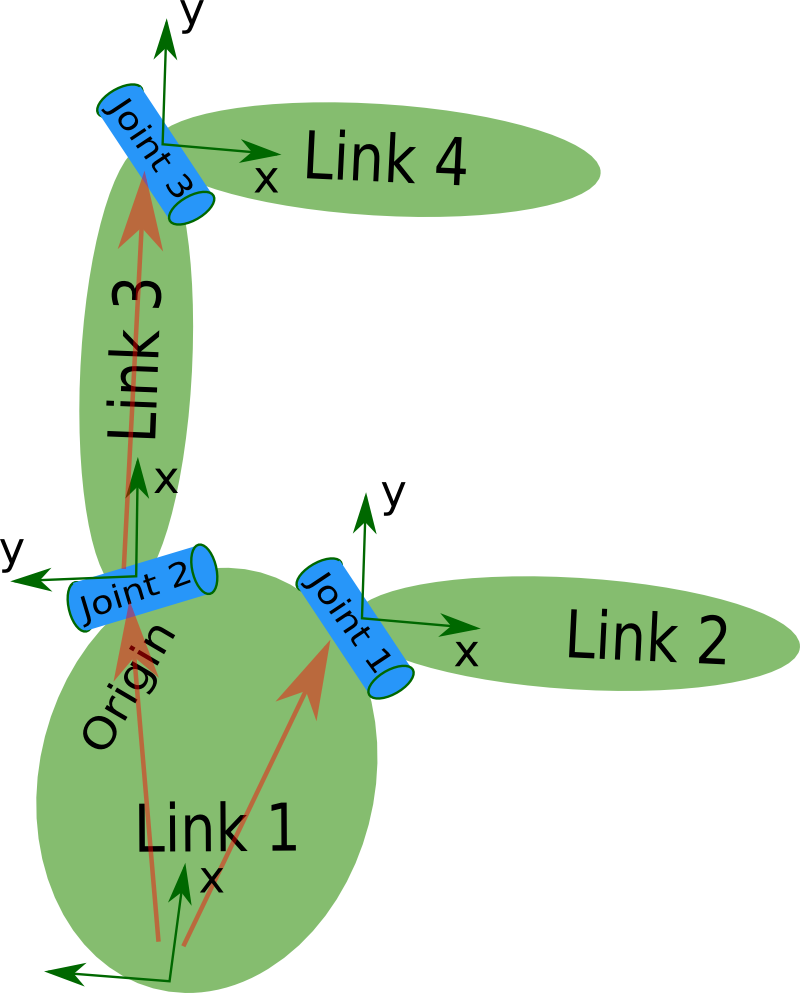
\includegraphics[height=0.3\textwidth]{img/links-joints.png}
% 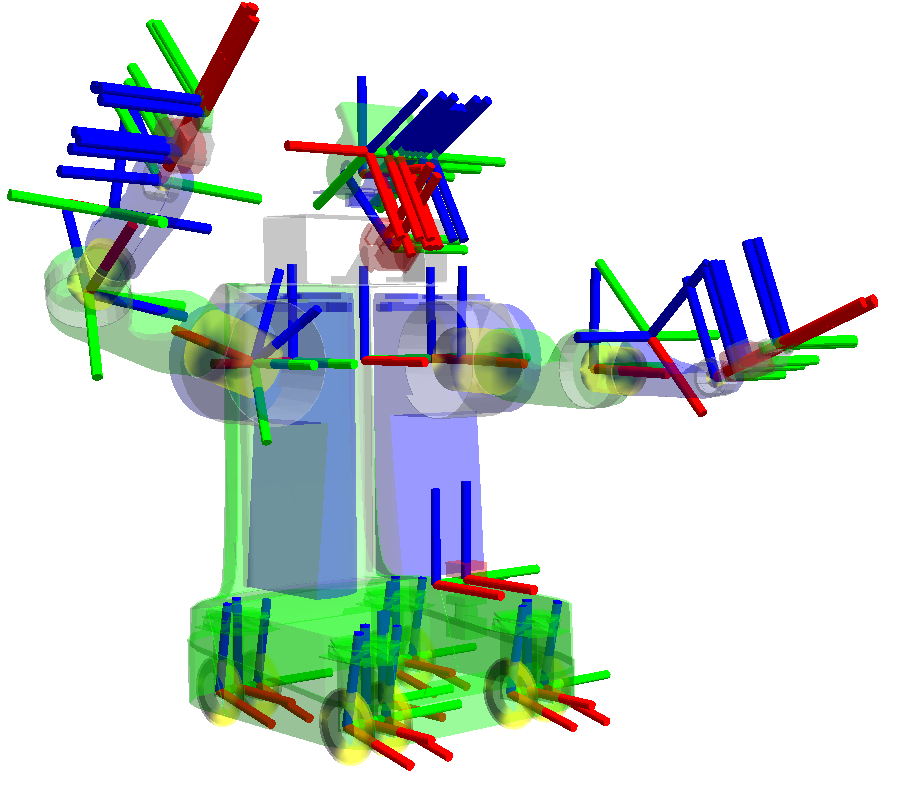
\includegraphics[height=0.3\textwidth]{img/tf-frames.png}
% \end{center}

Pose data is saved in \mongodb collections named ``tf'', the format is described below.

%%%%%%%%%%%%%%%%%%%%%%%%%%%%%%%%%
%%%%%%%%%%%%%%%%%%%%%%%%%%%%%%%%%
\subsubsection{Format}
The pose data structure has
fields for encoding the translation and rotation of a coordinate frame.
The parent frame and time stamp of pose estimation
are stored in the \emph{header} field of the data structure.
The transform coordinate frame is assigned to the \emph{child\_frame\_id} field.

The data is stored in the DB collection as array.
Each array holding pose estimates for distinct frames
at the same time stamp.
For indexed search, it is important that each array
member has the same time stamp. \\

\def\arraystretch{1.1}%
\begin{figure}[htb]
\begin{center}\begin{tabular}{ >{\ttfamily}p{3.5cm} >{\ttfamily}p{2cm} p{5cm} }
\toprule
\bf Field   & \bf Type & \bf Description \\ \midrule
tf			& [dict]	& -- \\
\ \ header		& dict		& -- \\
\ \ \ \ seq		& uint32	& consecutively increasing ID \\
\ \ \ \ stamp		& time		& time stamp of this transform \\
\ \ \ \ frame\_id	& string	& parent coordinate frame of this transform \\
\ \ child\_frame\_id	& string	& coordinate frame of this transform \\
\ \ transform		& dict		& -- \\
\ \ \ \ translation	& dict		& -- \\
\ \ \ \ \ \ x		& float64	& \emph{x} axis translation \\
\ \ \ \ \ \ y		& float64	& \emph{y} axis translation \\
\ \ \ \ \ \ z		& float64	& \emph{z} axis translation \\
\ \ \ \ rotation	& dict		& -- \\
\ \ \ \ \ \ x		& float64	& \emph{x} component of quaternion \\
\ \ \ \ \ \ y		& float64	& \emph{y} component of quaternion \\
\ \ \ \ \ \ z		& float64	& \emph{z} component of quaternion \\
\ \ \ \ \ \ w		& float64	& \emph{w} component of quaternion \\
\bottomrule
\end{tabular}\end{center}
\caption{The pose data structure in the \ease system.}
\label{fig:pose_data}
\end{figure}

Note that static frames may be recorded at lower frequency --
about every two seconds.
This usually reduces the data size significantly.
At the moment, no other motion data compression,
such as motion JPEG, is supported.

% From ``Compression of Motion Capture Databases'' Okan Arikan
% The biggest goal of compression is creating a compressed rep-
% resentation of motion that is perceptually as close to the original
% motion as possible. As we will explore later in this paper, a small
% numerical error does not necessarily correspond to a perceptually
% close motion. We would like compression and decompression to be
% as quick as possible. In practice motion capture databases can be
% very big. Therefore another goal for compression and decompres-
% sion is to be able to process without holding the entire database in
% the memory, which may not be possible. Depending on the appli-
% cation we may want to “stream” the data so that the decompressor
% can decode incrementally. We may also want to be able to decode a
% piece of the database without having to decompress any other mo-
% tion

%%%%%%%%%%%%%%%%%%%%%%%%%%%%%%%%%
%%%%%%%%%%%%%%%%%%%%%%%%%%%%%%%%%
\subsubsection{Symbol Abstraction}
%%%%%%%%%%%%%%%%%%%%%%%%%%%%%%%%%
\begin{center}
\begin{tabular}{ >{\ttfamily\bf}p{3.5cm} >{\ttfamily}p{8.2cm} }
\toprule
Module  & knowrob\_objects\footnote{\url{https://github.com/knowrob/knowrob/tree/master/knowrob\_objects}} \\
Symbols & object pose \\
Implementation & Prolog \\
\bottomrule
\end{tabular}
\end{center}
\begin{description}
\item[\textbf{belief\_at(Object, [Parent,Child,Translation,Rotation], Instant)}]
This temporal predicate computes a Prolog-based pose representation (2nd argument)
for a named object (1st argument). Time is supplied to the predicate as time stamp
(3rd argument).
\end{description}

%%%%%%%%%%%%%%%%%%%%%%%%%%%%%%%%%
\begin{center}
\begin{tabular}{ >{\ttfamily\bf}p{3.5cm} >{\ttfamily}p{8.2cm} }
\toprule
Module  & comp\_spatial\footnote{\url{https://github.com/knowrob/knowrob/tree/master/comp\_spatial}} \\
Symbols & spatial relations \\
Implementation & Prolog \\
\bottomrule
\end{tabular}
\end{center}


\begin{description}
\item[\textbf{comp\_inCenterOf(Inner,Outer,Interval)}]
Check if \owlClass{Inner} is in the center of \owlClass{Outer}.
Currently does not take the orientation into account, only the position and dimension.
Computes the \owlPredicate{inCenterOf} relation.

\item[\textbf{comp\_inFrontOf(Front,Back,Interval)}]
Check if \owlClass{Front} is in front of \owlClass{Back}.
Currently does not take the orientation
into account, only the position and dimension.
Computes the \owlPredicate{inFrontOf-Generally} relation.

\item[\textbf{comp\_inContGeneric(Inner,Outer,Interval)}]
True iff the object \owlClass{Inner} is inside 
of the bounding box of container \owlClass{Outer} during
the specified interval.
Computes the \owlPredicate{in-ContGeneric} relation.

\item[\textbf{comp\_onPhysical(Top,Bottom,Interval)}]
Check if \owlClass{Top} is in the area of and above \owlClass{Bottom}.
Computes the \owlPredicate{on-Physical} relation

\item[\textbf{comp\_above(Top,Bottom,Interval)}]
Check if \owlClass{Top} is in the area of and above \owlClass{Bottom}.
Computes the \owlPredicate{above-Generally} relation.

\item[\textbf{comp\_below(Bottom,Top,Interval)}]
Check if \owlClass{Top} is in the area of and above \owlClass{Bottom}.
Computes the \owlPredicate{below-Generally} relation.

\item[\textbf{comp\_toTheLeftOf(Left,Right,Interval)}]
Check if \owlClass{Left} is to the left of \owlClass{Right}.
Currently does not take the orientation
into account, only the position and dimension.
Computes the \owlPredicate{toTheLeftOf} relation.

\item[\textbf{comp\_toTheRightOf(Right,Left,Interval)}]
Check if \owlClass{Left} is to the left of \owlClass{Right}.
Currently does not take the orientation
into account, only the position and dimension.
Computes the \owlPredicate{toTheRightOf} relation.
\end{description}


%%%%%%%%%%%%%%%%%%%%%%%%%%%%%%%%%
%%%%%%%%%%%%%%%%%%%%%%%%%%%%%%%%%
% \section{Image Data}
% \input{content/neem-experience/image-data}

%%%%%%%%%%%%%%%%%%%%%%%%%%%%%%%%%
%%%%%%%%%%%%%%%%%%%%%%%%%%%%%%%%%
% \section{Gaze Data}
% \input{content/neem-experience/gaze-data}

%%%%%%%%%%%%%%%%%%%%%%%%%%%%%%%%%
%%%%%%%%%%%%%%%%%%%%%%%%%%%%%%%%%
% \section{EEG Data}
% \input{content/neem-experience/eeg-data}


\setcounter{section}{0}
\chapter{NEEM-Hub}
\label{ch:neemhub}
\chapterauthor{S. Koralewski}

\section{Publishing}
In this chapter we have to describe, how the NEEM narrative and NEEM experience should be represented e.g.\ using OWL and MongoDB and how the partners can upload those file to openEASE.

\section{Maintaining}


\setcounter{section}{0}
\chapter{NEEM-Acquisition}
\label{ch:acquisition}
\chapterauthor{S. Koralewski, A. Hawkin}

This chapter focuses on the acquisition process of \neems.
At first, we will provide the tools and procedures to acquire episodic memories from robots performing experiments.
The second section focuses on the \neem acquisition from virtual reality. 

%Each section will contain an example \neem to provide insights on, how the representation, described in the chapters \ref{ch:background}, \ref{ch:narrative} and \ref{ch:experience} is utilized to capture performed activities by robots or by humans. 
%In addition, each example \neem is available on the \neemhub for downloading.



\section{Data Structure}

We are using MongoDB to capture the data structures of the \neems.
If you will use the \knowrob interface to create your \neems then your \neem will consist of at least 3 folders - \textit{annotations}, \textit{inferred} and \textit{triples}.
The \neemnar and \neemexp are stored as a collection of BSON \footnote{http://bsonspec.org/faq.html} files.
Each folder should contain a BSON file and metafile stored as JSON. The metafile will include additional information related to \neems. This additional meta information is useful for searching \neem on \openease platform and hence needs to be provided by \neem creator while \neem acquisition time. An example of such information is as displayed below:

\begin{lstlisting}[language=json,firstnumber=1]
	{
		"_id" : ObjectId("5f22b1f512db5aed7cd1961b"), 
		"created_by" : "seba",
		"created_at" : "2020-07-21T06:54:25+00:00",
		"model_version" : "0.1",
		"description" : "NEEM for robot making pizza.",
		"keywords" : [	
		"Pizza",
		"Robot"
		],
		"url" : "Placeholder for the NEEM hub repository url",
		"name" : "NEEM for robot making pizza",
		"activity" : {
			"name" : "Pizza making",
			"url" : "Placeholder for the url/uri of Activity concept defined in ontology"    
		},
		"environment" : "Kitchen",
		"image" : "placeholder for image url for showing neem image on openEASE",  
		"agent" : "Robot"
	}
	
\end{lstlisting}

Each generated \neem stores also the complete state of the \soma ontology which was used during the acquisition process.
The benefit of this is that while loading a \neem, it is not required to keep track to load the correct \soma version.
In the following, we will give an overview which information is contained in those folders generated by \knowrob:


\begin{description}
	\item[\textbf{annotations}] The annotations collection contains annotations(comments) which are asserted to the concepts of the ontology.
	\item[\textbf{inferred}] The inferred collection contains triples which were inferred and not asserted during the logging process. Inference processes can be triggered when triples are asserted directly to the knowledge base.
	\item[\textbf{triples}] The triples collection contains all triples which were asserted into the knowledge base during run time.
\end{description}


\chapter{Robot \neems}

This chapter focuses on describing how to generate \neems~from robot 

\section{Prerequisite}

Before you are generating logs, make sure you are familiar with the Cognitive Robot Abstract Machine (\cram) system \url{http://cram-system.org/cram}.
In addition, you will need also a MongoDB Server with version 3.4.10.
Make sure you also installed Knowrob
https://github.com/knowrob/knowrob

and the following ontologies
https://github.com/ease-crc/cram\_knowledge
https://github.com/ease-crc/ease\_ontology

Having those components make sure before you run your cram plan, launch the \knowrob with the memory function via "roslaunch knowrob\_memory knowrob.launch"



\section{Generating Logs}
Intention of the logger is to log everything what is will be execute during the \cram action.
First it is required that you include "cram-cloud-logger" package in your \cram package, before you can start to create \neems.
After you included your the logger package, you need to set \textit{is-logging-enabled} to true via "(setf ccl::*is-logging-enabled* t)".
The only things left to do start the logging before the plan execution and after the execution, finishing it.
It can look like the following:
	(ccl::start-episode)
	(urdf-proj:with-simulated-robot (demo::demo-random nil ))
	(ccl::stop-episode)
	
The generate log file is stored per default in "~/knowrob-memory" 

\section{Data}
After you generate your first \neem~you will find a folder with a timestamp store in the "~/knowrob-memory" folder (per default).
This folder contains the \neemnar and \neemexp . The \neemnar is represented in the "beliefstate.owl". The triple store and the \neemexp are stored in the "roslog" folder. The triple store is stored in the "triples.bson". The other bsons files are presentening the logged rostopics. More about the rostopics is stated in Section \todo{put reference to rostopic section}

\section{Log own designed plans}
The disadvantage of having a strong semantic knowledge representation is that our ontology.
Currently, we focused on the support on setting-up and cleaning-up a table.
If you want for instance create \neems for an autonomous car, you will need to extend the \ease ontologies and the logger with your required actions, parameters etc.
In the following subsection, we will describe how you can add the required stuff so they are semantical log.
In general, please feel free to share your changes with us in form of an pull request to our repositories.
So we can provide you feedback and your help us to extend the features

\subsection{Adding New Tasks}
The most obvious requirement is to define your tasks.
A task might be something like cutting, stopping or accelerating.
To be able to semantaclly log the task, you will need first define the task in the \easeAct.
Make sure that the new action is a child of the \textit{CommunicationTask}, \textit{MentalTask} or \textit{PhysicalTask}.
If you will try to log unknown task, there will be logged as \textit{PhysicalTask}.
The \textit{PlanExecution} instance pointing to that \textit{PhysicalTask} , will have a comment attached with the statement "Unknown Action: <CRAM-ACTION-NAME>".
After you add the new action to the ontology, please open the "knowrob-action-name-handler.lisp" in the cram-cloud-logger package and add your new action in the format "(CRAM-ACTION-NAME EASE-ONTOLOGY-NAME)".
If this step you added successfully the support of the new action to the logger.

\subsection{Adding New Objects}
Unknown object will be logged as \textit{DesignedArtifact} with the comment attached "Unknown Object: CRAM-OBJECT-TYPE"
To add your object to the ontology, you need to add it in the \easeObj.
Afterwards, open the "utils-for-perform.lisp" in the 
cram-cloud-logger package and include the new object in the hash table generate in "get-ease-object-lookup-table" where the key is the CRAM-OBJECT-TYPE and the value is the uri to the object concept created in \easeObj.

\subsection{Adding New Failure}
Unknown failures will be logged as \textit{Failure} with the comment attached "Unknown failure: CRAM-FAILURE-NAME".
To integrate your new \cram failures in to the ontology, you need to add your new failures into the \cramOwl.
Afterwards, open "failure-handler.lisp" in the cram-cloud-logger package and your new action in the format "(CRAM-FAILURE-NAME CRAM-ONTOLOGY-NAME)".	

\subsection{Adding New Rostopic}
Per default, we log the rostopics \tf and tf\_static.
If you need to log additional topics, open "memory.pl" in the "knowrob\_memory" package from \knowrob and include your topic in the "mem\_episode\_start(Episode)" function.
After the \neem generation, the data will be stored in the created \neem folder under the file "roslog/<rostopic>.bson".

\subsection{Adding New Parameters}
Unknown parameters will be logged as comment attached to the corresponding \textit{PlanExecution} instance.
The comment statement "Unknown Parameter: PARAMETER-NAME  -\#\#\#\#- PARAMETER-VALUE/>"
The current parameter types are represented 

\todo{@Ontology group: Please make sure that is available in the ontology }

\begin{enumerate} 
	\item Integer/Floats
	\item Posen
	\item Spatial Relations
	\item Link to entities of other ontologies such as http://knowrob.org/kb/PR2.owl\#pr2\_right\_arm
\end{enumerate}

Before you want to model your parameter what data type your parameter is.
If it is a complex object, you need to consider how you want to to represent it an the ontology.
For simpler representaion such has a discrete domain representation, you might represented as the domain values as \textit{Region} and add the model the parameter as a subconcept of \textit{Parameter}.
More information about the concepts \textit{Region} and \textit{Parameter} can be found in \todo{ reference to Region and parameter}.


\subsection{Adding New Reasoning Tasks}
\todo{@Ontology group: How to log the result of the reasoning query ?}



\section{Next steps}
After you have generate your \neem, you can use the tool \todo{Add neem2narrative} to generate an cvs file for your \neem.
Keep in mind that the csv is a abstraction of \neemnar and can be used to make data-mining on explicit knowledge.
For more sophisticated analysis, you will need to use \knowrob. 
We use this general analysis to identify bottlenecks in our plan execution.
We also showed that with a collection of \neems we are able to improve the robot's performance.
\todo{Af}
The tools for the feature extraction can be found here \todo{Add link}
Now that you we encourage you to generate your \neems and share them via our \neemhub.

\subsection{VR \neems}



%\chapter{Application}
\section{Question Answering}
\section{Machine Learning}

%\chapter{Future Work}

\section{NEEM-Experience}
\begin{enumerate}
	\item Logging Images
	\item CostMaps
\end{enumerate}

\section{NEEM-Narrative}
\begin{enumerate}
	\item Logging Reasoning Tasks
\end{enumerate}

\cleardoublepage
\bibliography{neem}
\bibliographystyle{plain}

%\setcounter{section}{0}
%\chapter{Appendix}
\label{app:complete_pub_list}

\section{NEEM Vocabulary}
\label{appendix:section1}
\pagestyle{fancy} 
\newcommand{\appendixstyle}[2]{\textbf{#1}\markboth{#1}{#1}\ {#2}}

\begin{pythontexcustomcode}{py}
import sys
sys.path.append("../../docs")
from owl_reader import OWLReader

OWL_FILES=[
    "http://www.ontologydesignpatterns.org/ont/dul/DUL.owl",
    "http://www.ease-crc.org/ont/SOMA.owl"
]

reader = OWLReader(OWL_FILES)
\end{pythontexcustomcode}

%\raggedright
\begin{multicols}{2}

\begin{pycode}
reader.get_classes()
\end{pycode}

\end{multicols}

\end{document}
